\documentclass[]{article}
\usepackage{lmodern}
\usepackage{amssymb,amsmath}
\usepackage{ifxetex,ifluatex}
\usepackage{fixltx2e} % provides \textsubscript
\ifnum 0\ifxetex 1\fi\ifluatex 1\fi=0 % if pdftex
  \usepackage[T1]{fontenc}
  \usepackage[utf8]{inputenc}
\else % if luatex or xelatex
  \ifxetex
    \usepackage{mathspec}
  \else
    \usepackage{fontspec}
  \fi
  \defaultfontfeatures{Ligatures=TeX,Scale=MatchLowercase}
  \newcommand{\euro}{€}
\fi
% use upquote if available, for straight quotes in verbatim environments
\IfFileExists{upquote.sty}{\usepackage{upquote}}{}
% use microtype if available
\IfFileExists{microtype.sty}{%
\usepackage{microtype}
\UseMicrotypeSet[protrusion]{basicmath} % disable protrusion for tt fonts
}{}
\usepackage[margin=1in]{geometry}
\usepackage{hyperref}
\PassOptionsToPackage{usenames,dvipsnames}{color} % color is loaded by hyperref
\hypersetup{unicode=true,
            pdftitle={R-code for Consequences of stage- and sex-specific demography on the adult sex ratio of a polygamous bird population},
            pdfauthor={Luke J. Eberhart-Phillips, Clemens Küpper, Tom E. X. Miller, Medardo Cruz-López, Kathryn Maher, Natalie dos Remedios, Martin A. Stoffel, Joseph I. Hoffman, Oliver Krüger, Tamás Székely},
            pdfborder={0 0 0},
            breaklinks=true}
\urlstyle{same}  % don't use monospace font for urls
\usepackage{color}
\usepackage{fancyvrb}
\newcommand{\VerbBar}{|}
\newcommand{\VERB}{\Verb[commandchars=\\\{\}]}
\DefineVerbatimEnvironment{Highlighting}{Verbatim}{commandchars=\\\{\}}
% Add ',fontsize=\small' for more characters per line
\usepackage{framed}
\definecolor{shadecolor}{RGB}{248,248,248}
\newenvironment{Shaded}{\begin{snugshade}}{\end{snugshade}}
\newcommand{\KeywordTok}[1]{\textcolor[rgb]{0.13,0.29,0.53}{\textbf{{#1}}}}
\newcommand{\DataTypeTok}[1]{\textcolor[rgb]{0.13,0.29,0.53}{{#1}}}
\newcommand{\DecValTok}[1]{\textcolor[rgb]{0.00,0.00,0.81}{{#1}}}
\newcommand{\BaseNTok}[1]{\textcolor[rgb]{0.00,0.00,0.81}{{#1}}}
\newcommand{\FloatTok}[1]{\textcolor[rgb]{0.00,0.00,0.81}{{#1}}}
\newcommand{\ConstantTok}[1]{\textcolor[rgb]{0.00,0.00,0.00}{{#1}}}
\newcommand{\CharTok}[1]{\textcolor[rgb]{0.31,0.60,0.02}{{#1}}}
\newcommand{\SpecialCharTok}[1]{\textcolor[rgb]{0.00,0.00,0.00}{{#1}}}
\newcommand{\StringTok}[1]{\textcolor[rgb]{0.31,0.60,0.02}{{#1}}}
\newcommand{\VerbatimStringTok}[1]{\textcolor[rgb]{0.31,0.60,0.02}{{#1}}}
\newcommand{\SpecialStringTok}[1]{\textcolor[rgb]{0.31,0.60,0.02}{{#1}}}
\newcommand{\ImportTok}[1]{{#1}}
\newcommand{\CommentTok}[1]{\textcolor[rgb]{0.56,0.35,0.01}{\textit{{#1}}}}
\newcommand{\DocumentationTok}[1]{\textcolor[rgb]{0.56,0.35,0.01}{\textbf{\textit{{#1}}}}}
\newcommand{\AnnotationTok}[1]{\textcolor[rgb]{0.56,0.35,0.01}{\textbf{\textit{{#1}}}}}
\newcommand{\CommentVarTok}[1]{\textcolor[rgb]{0.56,0.35,0.01}{\textbf{\textit{{#1}}}}}
\newcommand{\OtherTok}[1]{\textcolor[rgb]{0.56,0.35,0.01}{{#1}}}
\newcommand{\FunctionTok}[1]{\textcolor[rgb]{0.00,0.00,0.00}{{#1}}}
\newcommand{\VariableTok}[1]{\textcolor[rgb]{0.00,0.00,0.00}{{#1}}}
\newcommand{\ControlFlowTok}[1]{\textcolor[rgb]{0.13,0.29,0.53}{\textbf{{#1}}}}
\newcommand{\OperatorTok}[1]{\textcolor[rgb]{0.81,0.36,0.00}{\textbf{{#1}}}}
\newcommand{\BuiltInTok}[1]{{#1}}
\newcommand{\ExtensionTok}[1]{{#1}}
\newcommand{\PreprocessorTok}[1]{\textcolor[rgb]{0.56,0.35,0.01}{\textit{{#1}}}}
\newcommand{\AttributeTok}[1]{\textcolor[rgb]{0.77,0.63,0.00}{{#1}}}
\newcommand{\RegionMarkerTok}[1]{{#1}}
\newcommand{\InformationTok}[1]{\textcolor[rgb]{0.56,0.35,0.01}{\textbf{\textit{{#1}}}}}
\newcommand{\WarningTok}[1]{\textcolor[rgb]{0.56,0.35,0.01}{\textbf{\textit{{#1}}}}}
\newcommand{\AlertTok}[1]{\textcolor[rgb]{0.94,0.16,0.16}{{#1}}}
\newcommand{\ErrorTok}[1]{\textcolor[rgb]{0.64,0.00,0.00}{\textbf{{#1}}}}
\newcommand{\NormalTok}[1]{{#1}}
\usepackage{graphicx,grffile}
\makeatletter
\def\maxwidth{\ifdim\Gin@nat@width>\linewidth\linewidth\else\Gin@nat@width\fi}
\def\maxheight{\ifdim\Gin@nat@height>\textheight\textheight\else\Gin@nat@height\fi}
\makeatother
% Scale images if necessary, so that they will not overflow the page
% margins by default, and it is still possible to overwrite the defaults
% using explicit options in \includegraphics[width, height, ...]{}
\setkeys{Gin}{width=\maxwidth,height=\maxheight,keepaspectratio}
\setlength{\parindent}{0pt}
\setlength{\parskip}{6pt plus 2pt minus 1pt}
\setlength{\emergencystretch}{3em}  % prevent overfull lines
\providecommand{\tightlist}{%
  \setlength{\itemsep}{0pt}\setlength{\parskip}{0pt}}
\setcounter{secnumdepth}{0}

%%% Use protect on footnotes to avoid problems with footnotes in titles
\let\rmarkdownfootnote\footnote%
\def\footnote{\protect\rmarkdownfootnote}

%%% Change title format to be more compact
\usepackage{titling}

% Create subtitle command for use in maketitle
\newcommand{\subtitle}[1]{
  \posttitle{
    \begin{center}\large#1\end{center}
    }
}

\setlength{\droptitle}{-2em}
  \title{R-code for ``Consequences of stage- and sex-specific demography on the
adult sex ratio of a polygamous bird population''}
  \pretitle{\vspace{\droptitle}\centering\huge}
  \posttitle{\par}
  \author{Luke J. Eberhart-Phillips, Clemens Küpper, Tom E. X. Miller, Medardo
Cruz-López, Kathryn Maher, Natalie dos Remedios, Martin A. Stoffel,
Joseph I. Hoffman, Oliver Krüger, Tamás Székely}
  \preauthor{\centering\large\emph}
  \postauthor{\par}
  \predate{\centering\large\emph}
  \postdate{\par}
  \date{October 6, 2016}



% Redefines (sub)paragraphs to behave more like sections
\ifx\paragraph\undefined\else
\let\oldparagraph\paragraph
\renewcommand{\paragraph}[1]{\oldparagraph{#1}\mbox{}}
\fi
\ifx\subparagraph\undefined\else
\let\oldsubparagraph\subparagraph
\renewcommand{\subparagraph}[1]{\oldsubparagraph{#1}\mbox{}}
\fi

\begin{document}
\maketitle

In this document we provide all the necessary code for reproducing the
analyses presented in our paper. To access the dataset and Rmarkdown
file, please download this
\href{https://github.com/leberhartphillips/Ceuta_ASR_matrix_modeling}{GitHub}
repository. Simply follow the link and click on \emph{Download ZIP} on
the right-hand side of the page. An explanation of the files in the
repository can be found in the Readme file. Please don't hesitate to
contact Luke at \texttt{luke.eberhart{[}at{]}gmail.com} if you have any
questions.

The structure of the code we present here follows the analyses presented
in the \emph{Results} section of the paper.

\textbf{Prerequisites:}

\begin{itemize}
\tightlist
\item
  For running the complete code you need a \texttt{files} subfolder
  containing the raw data downloaded from \textbf{\texttt{data}} and
  \textbf{\texttt{output/bootstrap}} folders provided in the
  \href{https://github.com/leberhartphillips/Ceuta_ASR_matrix_modeling}{GitHub}
  repository.
\item
  The following packages are needed for analysis and can be easily
  installed from \href{http://cran.r-project.org/}{CRAN} by uncommenting
  the \texttt{install.packages} functions:
\end{itemize}

\begin{Shaded}
\begin{Highlighting}[]
\CommentTok{# install.packages("RMark")}
\CommentTok{# install.packages("stringr")}
\CommentTok{# install.packages("ggplot2")}
\CommentTok{# install.packages("dplyr")}
\CommentTok{# install.packages("grid")}
\CommentTok{# install.packages("gridExtra")}
\CommentTok{# install.packages("reshape2")}
\CommentTok{# install.packages("RColorBrewer")}
\CommentTok{# install.packages("Rmisc")}
\CommentTok{# install.packages("stats")}
\CommentTok{# install.packages("lme4")}
\CommentTok{# install.packages("magrittr")}
\KeywordTok{library}\NormalTok{(RMark) }
\KeywordTok{library}\NormalTok{(stringr)}
\KeywordTok{library}\NormalTok{(ggplot2)}
\KeywordTok{library}\NormalTok{(dplyr)}
\KeywordTok{library}\NormalTok{(gridExtra)}
\KeywordTok{library}\NormalTok{(grid)}
\KeywordTok{library}\NormalTok{(reshape2)}
\KeywordTok{library}\NormalTok{(RColorBrewer)}
\KeywordTok{library}\NormalTok{(Rmisc)}
\KeywordTok{library}\NormalTok{(stats)}
\KeywordTok{library}\NormalTok{(lme4)}
\KeywordTok{library}\NormalTok{(magrittr)}
\end{Highlighting}
\end{Shaded}

\begin{center}\rule{0.5\linewidth}{\linethickness}\end{center}

\subsection{Loading data}\label{loading-data}

To start, please load the following datasets into your R environment:

\begin{itemize}
\item
  \textbf{data/chick\_survival\_data.txt} contains the mark-recapture
  field data of chicks. Each row is a single uniquely marked chick
  identified by their \emph{ring}. The daily encounter history of an
  individual is expressed in their \emph{ch}, where a ``1'' indicates
  that an individual was encountered, ``0'' indicates it was not
  encountered, and ``.'' indicates that no survey took place on that
  day. \emph{year} indicates the year during which an individual was
  monitored and \emph{day\_of\_season} indicates the number of days
  since the start of the breeding season that an individual hatched.
  \emph{sex} describes the molecular sex-type of an individual with
  ``M'' for males and ``F'' for females. \emph{brood\_ID} is a unique
  brood identifier for the family from which a chick hatched.
\item
  \textbf{data/fledgling\_adult\_survival\_data.txt} contains the
  mark-recapture field data of fledglings and adults. Each row is a
  single uniquely marked individual identified by their \emph{ring}. The
  annual encounter history of an individual is expressed in their
  \emph{ch}, where a ``1'' indicates that an individual was encountered
  and ``0'' indicates it was not encountered. \emph{sex} describes the
  molecular sex-type of an individual with ``M'' for males and ``F'' for
  females. \emph{age} describes the stage at which an individual was
  initially captured, where ``J'' indicates it was first captured as a
  chick, and ``A'' indicates it was first captured as an adult.
\item
  \textbf{data/breeding\_data.txt} contains the individual reproductive
  histories of all marked breeding adults in the population. Each row is
  a nesting attempt uniquely identified by the nest \emph{ID}.
  \emph{no\_chicks} expresses the number of chicks that hatched from the
  nest. \emph{clutch\_size} indicates the number of eggs in the nest
  when it was initially discovered. \emph{year} describes the year in
  which the nest was active. \emph{male} and \emph{female} indicates the
  unique identity of the father and mother, respectively, with
  ``male\_NA'' and ``female\_NA'' describing cases in which the other
  mate was not identified.
\end{itemize}

\begin{Shaded}
\begin{Highlighting}[]
\KeywordTok{setwd}\NormalTok{(}\StringTok{"~/Dropbox/Luke/R_projects/Ceuta_ASR_Matrix_Modeling"}\NormalTok{)}
\NormalTok{chick <-}\StringTok{ }
\StringTok{  }\KeywordTok{read.table}\NormalTok{(}\StringTok{"data/chick_mark-recapture_data.txt"}\NormalTok{,}
             \DataTypeTok{header =} \OtherTok{TRUE}\NormalTok{, }\DataTypeTok{colClasses =} \KeywordTok{c}\NormalTok{(}\StringTok{"factor"}\NormalTok{, }\StringTok{"character"}\NormalTok{,}\StringTok{"factor"}\NormalTok{,}
                                           \StringTok{"numeric"}\NormalTok{,}\StringTok{"factor"}\NormalTok{,}\StringTok{"factor"}\NormalTok{, }\StringTok{"numeric"}\NormalTok{))}

\NormalTok{fledgling_adult <-}\StringTok{ }
\StringTok{  }\KeywordTok{read.table}\NormalTok{(}\StringTok{"data/fledgling_adult_mark-recapture_data.txt"}\NormalTok{,}
             \DataTypeTok{header =} \OtherTok{TRUE}\NormalTok{, }\DataTypeTok{colClasses =} \KeywordTok{c}\NormalTok{(}\StringTok{"factor"}\NormalTok{,}\StringTok{"character"}\NormalTok{,}\StringTok{"factor"}\NormalTok{,}\StringTok{"factor"}\NormalTok{))}

\NormalTok{breeding_data <-}\StringTok{ }
\StringTok{  }\KeywordTok{read.table}\NormalTok{(}\StringTok{"data/breeding_data.txt"}\NormalTok{, }
             \DataTypeTok{header =} \OtherTok{TRUE}\NormalTok{)}
\end{Highlighting}
\end{Shaded}

\begin{center}\rule{0.5\linewidth}{\linethickness}\end{center}

\subsection{Fecundity}\label{fecundity}

The objective here was to determine the average per capita annual
fecundity for females. This vital rate was then incorporated into the
two-sex matrix model. The second objective was to evalutate if the
distributions of male and female fecundity were different, which would
provide evidence of the polygamous nature of the snowy plover mating
system.

\textbf{Step one: wrangle the data}

Extract the female column from the breeding data, add a sex column,
extract the male colum, add a sex column, then stack these two
dataframes.

\begin{Shaded}
\begin{Highlighting}[]
\NormalTok{Sex <-}\StringTok{ }\KeywordTok{rep}\NormalTok{(}\StringTok{"Female"}\NormalTok{, }\KeywordTok{nrow}\NormalTok{(breeding_data))}
\NormalTok{Ring <-}\StringTok{ }\NormalTok{breeding_data$female}
\NormalTok{females <-}\StringTok{ }\KeywordTok{data.frame}\NormalTok{(Ring, Sex)}
\NormalTok{Sex <-}\StringTok{ }\KeywordTok{rep}\NormalTok{(}\StringTok{"Male"}\NormalTok{, }\KeywordTok{nrow}\NormalTok{(breeding_data))}
\NormalTok{Ring <-}\StringTok{ }\NormalTok{breeding_data$male}
\NormalTok{males <-}\StringTok{ }\KeywordTok{data.frame}\NormalTok{(Ring, Sex)}
\NormalTok{Individuals <-}\StringTok{ }\KeywordTok{rbind}\NormalTok{(males, females)}
\end{Highlighting}
\end{Shaded}

replicate each row by 2 then cbind the stacked dataframe from the
previous step

\begin{Shaded}
\begin{Highlighting}[]
\NormalTok{reproduction_df <-}\StringTok{ }\KeywordTok{cbind}\NormalTok{(breeding_data[}\KeywordTok{rep}\NormalTok{(}\KeywordTok{row.names}\NormalTok{(breeding_data), }\DecValTok{2}\NormalTok{), }
                                       \KeywordTok{c}\NormalTok{(}\StringTok{"no_chicks"}\NormalTok{, }\StringTok{"clutch_size"}\NormalTok{, }\StringTok{"brood_ID"}\NormalTok{, }\StringTok{"year"}\NormalTok{)],}
                      \NormalTok{Individuals)}
\end{Highlighting}
\end{Shaded}

change the order of the sex levels, so that females are first (for the
plot)

\begin{Shaded}
\begin{Highlighting}[]
\NormalTok{reproduction_df$Sex <-}\StringTok{ }\KeywordTok{factor}\NormalTok{(reproduction_df$Sex, }\DataTypeTok{levels =} \KeywordTok{c}\NormalTok{(}\StringTok{"Female"}\NormalTok{, }\StringTok{"Male"}\NormalTok{))}
\end{Highlighting}
\end{Shaded}

subset the data to remove entries that have a NA in the Ring column

\begin{Shaded}
\begin{Highlighting}[]
\NormalTok{reproduction_df <-}\StringTok{ }\NormalTok{reproduction_df[!}\KeywordTok{is.na}\NormalTok{(reproduction_df$Ring),]}
\end{Highlighting}
\end{Shaded}

subset the data to remove entries that have a NA in the no-chicks column

\begin{Shaded}
\begin{Highlighting}[]
\NormalTok{reproduction_df <-}\StringTok{ }\NormalTok{reproduction_df[!}\KeywordTok{is.na}\NormalTok{(reproduction_df$no_chicks),]}
\end{Highlighting}
\end{Shaded}

group data according to Year, Sex, then Ring

\begin{Shaded}
\begin{Highlighting}[]
\NormalTok{reproduction_df <-}\StringTok{ }\NormalTok{dplyr::}\KeywordTok{group_by}\NormalTok{(reproduction_df, year, Sex, Ring)}
\end{Highlighting}
\end{Shaded}

sum the total chicks produced per bird each year

\begin{Shaded}
\begin{Highlighting}[]
\NormalTok{reproduction_df_sum <-}\StringTok{ }
\StringTok{  }\NormalTok{dplyr::}\KeywordTok{ungroup}\NormalTok{(dplyr::}\KeywordTok{summarise}\NormalTok{(reproduction_df, }
                           \DataTypeTok{total_chicks_p_year =} \KeywordTok{sum}\NormalTok{(}\KeywordTok{as.numeric}\NormalTok{(no_chicks))))}
\end{Highlighting}
\end{Shaded}

\textbf{Step two: calculate fecundity}

calculate avg total chicks produced per bird in each year

\begin{Shaded}
\begin{Highlighting}[]
\NormalTok{fecundity_annual_summary <-}\StringTok{ }
\StringTok{  }\NormalTok{Rmisc::}\KeywordTok{summarySE}\NormalTok{(reproduction_df_sum, }\DataTypeTok{measurevar =} \StringTok{"total_chicks_p_year"}\NormalTok{, }
                   \DataTypeTok{groupvars =} \KeywordTok{c}\NormalTok{(}\StringTok{"Sex"}\NormalTok{, }\StringTok{"year"}\NormalTok{))}
\end{Highlighting}
\end{Shaded}

group data according to Sex then Ring

\begin{Shaded}
\begin{Highlighting}[]
\NormalTok{reproduction_df_sum <-}\StringTok{ }\NormalTok{dplyr::}\KeywordTok{group_by}\NormalTok{(reproduction_df_sum, Sex, Ring)}
\end{Highlighting}
\end{Shaded}

calculate avg total chicks produced per bird each year

\begin{Shaded}
\begin{Highlighting}[]
\NormalTok{reproduction_df_sum_avg <-}\StringTok{ }
\StringTok{  }\NormalTok{dplyr::}\KeywordTok{ungroup}\NormalTok{(dplyr::}\KeywordTok{summarise}\NormalTok{(reproduction_df_sum, }
                           \DataTypeTok{avg_chicks_p_year =} \KeywordTok{mean}\NormalTok{(}\KeywordTok{as.numeric}\NormalTok{(total_chicks_p_year))))}
\end{Highlighting}
\end{Shaded}

summarize the avg annual no\_chicks by sex

\begin{Shaded}
\begin{Highlighting}[]
\NormalTok{fecundity_sex_summary <-}\StringTok{ }
\StringTok{  }\NormalTok{Rmisc::}\KeywordTok{summarySE}\NormalTok{(fecundity_annual_summary, }
                   \DataTypeTok{measurevar =} \StringTok{"total_chicks_p_year"}\NormalTok{, }\DataTypeTok{groupvars =} \KeywordTok{c}\NormalTok{(}\StringTok{"Sex"}\NormalTok{))}
\end{Highlighting}
\end{Shaded}

Determine how many individuals were included in the analysis

\begin{Shaded}
\begin{Highlighting}[]
\NormalTok{sample_sizes_sex <-}\StringTok{ }
\StringTok{  }\KeywordTok{aggregate}\NormalTok{(Ring ~}\StringTok{ }\NormalTok{Sex, }\DataTypeTok{data =} \NormalTok{reproduction_df_sum_avg, }\DataTypeTok{FUN =} \NormalTok{function(x)\{}\KeywordTok{NROW}\NormalTok{(x)\})}
\end{Highlighting}
\end{Shaded}

specify the color pallete to use for the plot

\begin{Shaded}
\begin{Highlighting}[]
\NormalTok{cbPalette <-}\StringTok{ }\NormalTok{RColorBrewer::}\KeywordTok{brewer.pal}\NormalTok{(}\DecValTok{8}\NormalTok{, }\StringTok{"Dark2"}\NormalTok{)[}\KeywordTok{c}\NormalTok{(}\DecValTok{2}\NormalTok{,}\DecValTok{1}\NormalTok{)]}
\end{Highlighting}
\end{Shaded}

\textbf{Step three: plot the sex-specific distributions}

\begin{Shaded}
\begin{Highlighting}[]
\NormalTok{ggplot2::}\KeywordTok{ggplot}\NormalTok{() +}
\StringTok{  }\KeywordTok{geom_boxplot}\NormalTok{(}\KeywordTok{aes}\NormalTok{(}\DataTypeTok{y =} \NormalTok{avg_chicks_p_year, }\DataTypeTok{x =} \NormalTok{Sex, }\DataTypeTok{fill =} \NormalTok{Sex), }
               \DataTypeTok{data =} \NormalTok{reproduction_df_sum_avg, }\DataTypeTok{size =} \NormalTok{.}\DecValTok{3}\NormalTok{, }\DataTypeTok{alpha =} \FloatTok{0.6}\NormalTok{) +}
\StringTok{  }\KeywordTok{geom_text}\NormalTok{(}\DataTypeTok{data =} \NormalTok{sample_sizes_sex, }\DataTypeTok{size =} \DecValTok{3}\NormalTok{, }
            \KeywordTok{aes}\NormalTok{(}\DataTypeTok{y =} \KeywordTok{c}\NormalTok{(}\FloatTok{6.5}\NormalTok{, }\FloatTok{6.5}\NormalTok{), }\DataTypeTok{x =} \KeywordTok{c}\NormalTok{(}\FloatTok{1.12}\NormalTok{, }\FloatTok{2.12}\NormalTok{), }\DataTypeTok{label =} \NormalTok{Ring)) +}
\StringTok{  }\KeywordTok{annotate}\NormalTok{(}\StringTok{"text"}\NormalTok{, }\DataTypeTok{x =} \KeywordTok{c}\NormalTok{(}\FloatTok{0.92}\NormalTok{, }\FloatTok{1.92}\NormalTok{), }\DataTypeTok{y =} \KeywordTok{c}\NormalTok{(}\FloatTok{6.5}\NormalTok{, }\FloatTok{6.5}\NormalTok{), }\DataTypeTok{label =} \StringTok{"n = "}\NormalTok{, }
           \DataTypeTok{size =} \DecValTok{3}\NormalTok{) +}
\StringTok{  }\KeywordTok{theme_bw}\NormalTok{() +}
\StringTok{  }\KeywordTok{theme}\NormalTok{(}\DataTypeTok{text=}\KeywordTok{element_text}\NormalTok{(}\DataTypeTok{size=}\DecValTok{16}\NormalTok{),}
        \DataTypeTok{legend.position =} \StringTok{"none"}\NormalTok{,}
        \DataTypeTok{axis.title.x =} \KeywordTok{element_blank}\NormalTok{(),}
        \DataTypeTok{axis.text.x  =} \KeywordTok{element_text}\NormalTok{(}\DataTypeTok{size =} \DecValTok{10}\NormalTok{), }
        \DataTypeTok{axis.title.y =} \KeywordTok{element_text}\NormalTok{(}\DataTypeTok{size =} \DecValTok{12}\NormalTok{, }
                                    \DataTypeTok{margin =} \KeywordTok{margin}\NormalTok{(}\DecValTok{0}\NormalTok{, }\DecValTok{15}\NormalTok{, }\DecValTok{0}\NormalTok{, }\DecValTok{0}\NormalTok{)),}
        \DataTypeTok{axis.text.y =} \KeywordTok{element_text}\NormalTok{(}\DataTypeTok{size =} \DecValTok{10}\NormalTok{), }
        \DataTypeTok{panel.grid.major =} \KeywordTok{element_blank}\NormalTok{(),}
        \DataTypeTok{panel.grid.minor =} \KeywordTok{element_blank}\NormalTok{(),}
        \DataTypeTok{axis.ticks.y =} \KeywordTok{element_line}\NormalTok{(}\DataTypeTok{size =} \FloatTok{0.5}\NormalTok{, }\DataTypeTok{colour =} \StringTok{"grey40"}\NormalTok{),}
        \DataTypeTok{axis.ticks.length =} \KeywordTok{unit}\NormalTok{(}\FloatTok{0.2}\NormalTok{, }\StringTok{"cm"}\NormalTok{),}
        \DataTypeTok{axis.ticks.x =} \KeywordTok{element_blank}\NormalTok{(),}
        \DataTypeTok{panel.border =} \KeywordTok{element_rect}\NormalTok{(}\DataTypeTok{linetype =} \StringTok{"solid"}\NormalTok{, }\DataTypeTok{colour =} \StringTok{"grey"}\NormalTok{)) +}
\StringTok{  }\KeywordTok{scale_fill_manual}\NormalTok{(}\DataTypeTok{values =} \NormalTok{cbPalette) +}
\StringTok{  }\KeywordTok{ylab}\NormalTok{(}\StringTok{"Per capita annual hatchlings parented"}\NormalTok{) +}
\StringTok{  }\KeywordTok{scale_y_continuous}\NormalTok{(}\DataTypeTok{limits =} \KeywordTok{c}\NormalTok{(}\DecValTok{0}\NormalTok{, }\FloatTok{6.5}\NormalTok{))}
\end{Highlighting}
\end{Shaded}

\begin{center}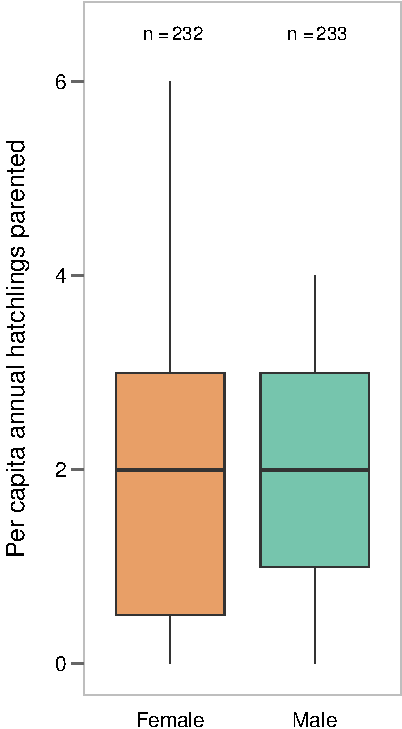
\includegraphics{Ceuta_ASR_Matrix_Modeling_files/figure-latex/unnamed-chunk-17-1} \end{center}

\textbf{Step four: statistical testing of sex-specific variance in
fecundity}

Run F-test to assess sex-specific variation in per capita fecundity

\begin{Shaded}
\begin{Highlighting}[]
\NormalTok{reproduction_df_sum_avg <-}\StringTok{ }\KeywordTok{as.data.frame}\NormalTok{(reproduction_df_sum_avg)}
\KeywordTok{var.test}\NormalTok{(reproduction_df_sum_avg[}\KeywordTok{which}\NormalTok{(reproduction_df_sum_avg$Sex ==}\StringTok{ "Female"}\NormalTok{),}
                                 \KeywordTok{c}\NormalTok{(}\StringTok{"avg_chicks_p_year"}\NormalTok{)],}
         \NormalTok{reproduction_df_sum_avg[}\KeywordTok{which}\NormalTok{(reproduction_df_sum_avg$Sex ==}\StringTok{ "Male"}\NormalTok{),}
                                 \KeywordTok{c}\NormalTok{(}\StringTok{"avg_chicks_p_year"}\NormalTok{)],}
         \DataTypeTok{alternative =} \StringTok{"greater"}\NormalTok{)}
\CommentTok{#> }
\CommentTok{#>  F test to compare two variances}
\CommentTok{#> }
\CommentTok{#> data:  reproduction_df_sum_avg[which(reproduction_df_sum_avg$Sex ==  and reproduction_df_sum_avg[which(reproduction_df_sum_avg$Sex ==     "Female"), c("avg_chicks_p_year")] and     "Male"), c("avg_chicks_p_year")]}
\CommentTok{#> F = 1.4651, num df = 231, denom df = 232, p-value = 0.0019}
\CommentTok{#> alternative hypothesis: true ratio of variances is greater than 1}
\CommentTok{#> 95 percent confidence interval:}
\CommentTok{#>  1.179765      Inf}
\CommentTok{#> sample estimates:}
\CommentTok{#> ratio of variances }
\CommentTok{#>            1.46513}
\end{Highlighting}
\end{Shaded}

Assign the value of female per capita annual fecundity to a constant
that will be included in the matrix

\begin{Shaded}
\begin{Highlighting}[]
\NormalTok{RF <-}\StringTok{ }\NormalTok{fecundity_sex_summary[}\DecValTok{1}\NormalTok{,}\DecValTok{3}\NormalTok{]}
\NormalTok{RF}
\CommentTok{#> [1] 2.03688}
\end{Highlighting}
\end{Shaded}

\begin{center}\rule{0.5\linewidth}{\linethickness}\end{center}

\subsection{Hatching sex ratio}\label{hatching-sex-ratio}

The hatching sex ratio represents ``rho'' in the matrix model and is
calculated from broods that met two criteria: 1) the brood size was the
modal clutch size (3 in the case of snowy plovers), and 2) chicks were
captured and sampled on the day of hatching. These criteria made sure to
control for post-hatch brood mixing.

\textbf{Step one: wrangle the data}

Subset the chick mark-recapture data so that only chicks captured on the
day of hatch are included. In this dataframe, the ``ch'' column refers
to the capture history of an individual on each day of its life as a
chick. Thus, if the first character of the ``ch'' string is a 1, it was
captured on the day of hatch and is included in the hatch sex ratio
dataset.

\begin{Shaded}
\begin{Highlighting}[]
\NormalTok{caught_at_hatch <-}\StringTok{ }\NormalTok{chick[}\KeywordTok{which}\NormalTok{(}\KeywordTok{substring}\NormalTok{(chick$ch, }\DecValTok{1}\NormalTok{, }\DecValTok{1}\NormalTok{) ==}\StringTok{ "1"}\NormalTok{),]}
\end{Highlighting}
\end{Shaded}

sum the number of chicks that are included for each hatch ID

\begin{Shaded}
\begin{Highlighting}[]
\NormalTok{brood_ID_count <-}\StringTok{ }
\NormalTok{caught_at_hatch %>%}\StringTok{ }
\StringTok{  }\NormalTok{dplyr::}\KeywordTok{count}\NormalTok{(brood_ID)}
\end{Highlighting}
\end{Shaded}

join this data to the subset capture data

\begin{Shaded}
\begin{Highlighting}[]
\NormalTok{caught_at_hatch <-}\StringTok{ }\NormalTok{dplyr::}\KeywordTok{left_join}\NormalTok{(caught_at_hatch, brood_ID_count, }\DataTypeTok{by =} \StringTok{"brood_ID"}\NormalTok{)}
\end{Highlighting}
\end{Shaded}

subset these data so that clutch size equals the number of chicks
sampled from each nest

\begin{Shaded}
\begin{Highlighting}[]
\NormalTok{HSR_df <-}\StringTok{ }\NormalTok{caught_at_hatch[}\KeywordTok{which}\NormalTok{(caught_at_hatch$clutch_size ==}\StringTok{ }\NormalTok{caught_at_hatch$n),]}
\end{Highlighting}
\end{Shaded}

make new columns ``Male'' and ``Female'' that have 1 or 0 to describe
the sex of the chick

\begin{Shaded}
\begin{Highlighting}[]
\NormalTok{HSR_df$male <-}\StringTok{ }\KeywordTok{ifelse}\NormalTok{(HSR_df$sex ==}\StringTok{ "M"}\NormalTok{, }\DecValTok{1}\NormalTok{, }\DecValTok{0}\NormalTok{)}
\NormalTok{HSR_df$female <-}\StringTok{ }\KeywordTok{ifelse}\NormalTok{(HSR_df$sex ==}\StringTok{ "F"}\NormalTok{, }\DecValTok{1}\NormalTok{, }\DecValTok{0}\NormalTok{)}
\end{Highlighting}
\end{Shaded}

define hatch ID as a factor

\begin{Shaded}
\begin{Highlighting}[]
\NormalTok{HSR_df$brood_ID <-}\StringTok{ }\KeywordTok{as.factor}\NormalTok{(HSR_df$brood_ID)}
\end{Highlighting}
\end{Shaded}

\textbf{Step two: mixed effects linear regression}

Brood ID is used as a random effect to control for the non-independence
of siblings

\begin{Shaded}
\begin{Highlighting}[]
\NormalTok{HSR_model <-}\StringTok{ }\NormalTok{lme4::}\KeywordTok{glmer}\NormalTok{(}\KeywordTok{cbind}\NormalTok{(male, female) ~}\StringTok{ }\NormalTok{(}\DecValTok{1}\NormalTok{|brood_ID),}
                     \DataTypeTok{data =} \NormalTok{HSR_df, }\DataTypeTok{family =} \NormalTok{binomial)}
\end{Highlighting}
\end{Shaded}

check out the model results. P = 0.588, therefore hatching sex ratio
doesn't deviate from parity

\begin{Shaded}
\begin{Highlighting}[]
\KeywordTok{summary}\NormalTok{(HSR_model)}
\CommentTok{#> Generalized linear mixed model fit by maximum likelihood (Laplace}
\CommentTok{#>   Approximation) [glmerMod]}
\CommentTok{#>  Family: binomial  ( logit )}
\CommentTok{#> Formula: cbind(male, female) ~ (1 | brood_ID)}
\CommentTok{#>    Data: HSR_df}
\CommentTok{#> }
\CommentTok{#>      AIC      BIC   logLik deviance df.resid }
\CommentTok{#>    475.0    482.7   -235.5    471.0      338 }
\CommentTok{#> }
\CommentTok{#> Scaled residuals: }
\CommentTok{#>    Min     1Q Median     3Q    Max }
\CommentTok{#> -0.971 -0.971 -0.971  1.030  1.030 }
\CommentTok{#> }
\CommentTok{#> Random effects:}
\CommentTok{#>  Groups   Name        Variance Std.Dev.}
\CommentTok{#>  brood_ID (Intercept) 0        0       }
\CommentTok{#> Number of obs: 340, groups:  brood_ID, 116}
\CommentTok{#> }
\CommentTok{#> Fixed effects:}
\CommentTok{#>             Estimate Std. Error z value Pr(>|z|)}
\CommentTok{#> (Intercept) -0.05884    0.10851  -0.542    0.588}
\end{Highlighting}
\end{Shaded}

calculate what the average hatching sex ratio is summarize the data so
that each row is a nest instead of an individual

\begin{Shaded}
\begin{Highlighting}[]
\NormalTok{HSR_df_summary <-}\StringTok{ }
\StringTok{  }\NormalTok{HSR_df %>%}\StringTok{ }
\StringTok{  }\NormalTok{dplyr::}\KeywordTok{group_by}\NormalTok{(brood_ID) %>%}
\StringTok{  }\NormalTok{dplyr::}\KeywordTok{summarise}\NormalTok{(}\DataTypeTok{no_males =} \KeywordTok{sum}\NormalTok{(male),}
                   \DataTypeTok{hatch_date_season =} \KeywordTok{min}\NormalTok{(day_of_season),}
                   \DataTypeTok{clutch_size =} \KeywordTok{mean}\NormalTok{(n),}
                   \DataTypeTok{year =} \KeywordTok{first}\NormalTok{(year))}
\end{Highlighting}
\end{Shaded}

calculate the proportion of the brood that was male

\begin{Shaded}
\begin{Highlighting}[]
\NormalTok{HSR_df_summary$prop_male <-}\StringTok{ }\NormalTok{HSR_df_summary$no_males/HSR_df_summary$clutch_size}
\end{Highlighting}
\end{Shaded}

calculate the average hatching sex ratio across all nests and assign the
result to a constant ``HSR'' to be used as rho in the matrix model

\begin{Shaded}
\begin{Highlighting}[]
\NormalTok{HSR <-}\StringTok{ }\KeywordTok{mean}\NormalTok{(HSR_df_summary$prop_male)}
\NormalTok{HSR}
\CommentTok{#> [1] 0.4856322}
\end{Highlighting}
\end{Shaded}

calculate the 95\% confidence interval of the hatching sex ratio

\begin{Shaded}
\begin{Highlighting}[]
\NormalTok{HSR_95CI <-}\StringTok{ }\KeywordTok{c}\NormalTok{(}\KeywordTok{mean}\NormalTok{(HSR_df_summary$prop_male)-}
\StringTok{                }\NormalTok{((}\KeywordTok{sd}\NormalTok{(HSR_df_summary$prop_male)/}
\StringTok{                    }\KeywordTok{sqrt}\NormalTok{(}\KeywordTok{length}\NormalTok{(HSR_df_summary$prop_male)))*}\FloatTok{1.96}\NormalTok{),}
              \KeywordTok{mean}\NormalTok{(HSR_df_summary$prop_male)+}
\StringTok{                }\NormalTok{((}\KeywordTok{sd}\NormalTok{(HSR_df_summary$prop_male)/}
\StringTok{                    }\KeywordTok{sqrt}\NormalTok{(}\KeywordTok{length}\NormalTok{(HSR_df_summary$prop_male)))*}\FloatTok{1.96}\NormalTok{))}
\end{Highlighting}
\end{Shaded}

\begin{center}\rule{0.5\linewidth}{\linethickness}\end{center}

\subsection{Bootstrapping proceedure}\label{bootstrapping-proceedure}

Specify where RMark should look on your computer for Program MARK. This
may vary based on your operating system (e.g., Windows, Linux, Mac OS X,
etc.). This \href{http://www.phidot.org/software/mark/rmark/}{website}
provides a nice workflow for installing Program MARK and linking it to
your R interface based on which operating system you have.

\begin{Shaded}
\begin{Highlighting}[]
\NormalTok{MarkPath <-}\StringTok{ "/usr/local/bin/mark"}
\NormalTok{MarkViewer <-}\StringTok{ "nano"}
\end{Highlighting}
\end{Shaded}

\textbf{Step one: Assign functions}

The following two functions are needed to setup the projection matrix
and estimate ASR. Load these before implementing the bootstrap
simulation.

\textbf{plover\_matrix()} builds the two-sex Lefkovitch matrix using the
vital rates specified in the \emph{demographic\_rates} object.

\begin{Shaded}
\begin{Highlighting}[]
\NormalTok{plover_matrix <-}\StringTok{ }
\StringTok{  }\NormalTok{function(demographic_rates)}
    \NormalTok{\{}
      \CommentTok{# Define plover life-stages of the Ceuta snowy plover matrix model}
      \NormalTok{stages <-}\StringTok{ }\KeywordTok{c}\NormalTok{(}\StringTok{"F_1st_yr"}\NormalTok{,  }\StringTok{"F_Adt"}\NormalTok{,  }\StringTok{"M_1st_yr"}\NormalTok{,  }\StringTok{"M_Adt"}\NormalTok{)}
      \CommentTok{# Build the 4x4 matrix}
      \NormalTok{result <-}\StringTok{ }
\StringTok{        }\KeywordTok{matrix}\NormalTok{(}\KeywordTok{c}\NormalTok{(}
                 \CommentTok{# top row of matrix}
                 \DecValTok{0}\NormalTok{, demographic_rates$RF *}\StringTok{ }\NormalTok{(}\DecValTok{1} \NormalTok{-}\StringTok{ }\NormalTok{HSR), }\DecValTok{0}\NormalTok{, }\DecValTok{0}\NormalTok{, }
                 \CommentTok{# second row of matrix}
                 \NormalTok{(demographic_rates$F_Chk_survl*demographic_rates$F_Fdg_survl),}
                 \NormalTok{demographic_rates$F_Adt_survl, }
                 \DecValTok{0}\NormalTok{, }\DecValTok{0}\NormalTok{,}
                 \CommentTok{# third row of matrix}
                 \DecValTok{0}\NormalTok{, demographic_rates$RF *}\StringTok{ }\NormalTok{HSR, }\DecValTok{0}\NormalTok{, }\DecValTok{0}\NormalTok{,}
                 \CommentTok{# fourth row of matrix}
                 \DecValTok{0}\NormalTok{, }\DecValTok{0}\NormalTok{, }
                 \NormalTok{(demographic_rates$M_Chk_survl*demographic_rates$M_Fdg_survl),}
                 \NormalTok{demographic_rates$M_Adt_survl),}
               \DataTypeTok{nrow =} \DecValTok{4}\NormalTok{, }\DataTypeTok{byrow =} \OtherTok{TRUE}\NormalTok{,}
               \DataTypeTok{dimnames =} \KeywordTok{list}\NormalTok{(stages, stages))}
      \NormalTok{result}
  \NormalTok{\}}
\end{Highlighting}
\end{Shaded}

\textbf{matrix\_ASR()} calculates the ASR of the population based on the
two-sex two-stage projection matrix built by the \emph{plover\_matrix()}
function. Arguments in the function include: \emph{A} is an two sex x by
x projection matrix \emph{n} is an x lengthed vector representing
starting stage distribution (the default is a vector with 10 individuals
in each stage)

\begin{Shaded}
\begin{Highlighting}[]
\NormalTok{matrix_ASR <-}\StringTok{ }
\StringTok{  }\NormalTok{function (A) }
  \NormalTok{\{}
    \CommentTok{# Number of stages in the matrix}
    \NormalTok{x <-}\StringTok{ }\KeywordTok{ncol}\NormalTok{(A) }
    \NormalTok{\{}
      \CommentTok{# determine the dominant eigen value and vector of the matrix}
      \NormalTok{ev <-}\StringTok{ }\KeywordTok{eigen}\NormalTok{(A)}
      \NormalTok{lmax <-}\StringTok{ }\KeywordTok{which.max}\NormalTok{(}\KeywordTok{Re}\NormalTok{(ev$values))}
      \NormalTok{W <-}\StringTok{ }\NormalTok{ev$vectors}
      \NormalTok{w <-}\StringTok{ }\KeywordTok{abs}\NormalTok{(}\KeywordTok{Re}\NormalTok{(W[, lmax]))}
      \KeywordTok{names}\NormalTok{(w) <-}\StringTok{ }\KeywordTok{colnames}\NormalTok{(A)}
    \CommentTok{# calculate the proportional stable stage distribution}
    \NormalTok{stable.stage <-}\StringTok{ }\NormalTok{w/}\KeywordTok{sum}\NormalTok{(w)}
    \CommentTok{# calc ASR as the proportion of the adult stable stage class that is male}
    \NormalTok{ASR <-}\StringTok{ }\NormalTok{stable.stage[x]/(stable.stage[x/}\DecValTok{2}\NormalTok{] +}\StringTok{ }\NormalTok{stable.stage[x])}
    
    \CommentTok{# make a list of results}
    \NormalTok{pop.proj <-}\StringTok{ }\KeywordTok{list}\NormalTok{(}\DataTypeTok{ASR =} \NormalTok{ASR,}
                     \DataTypeTok{stable.stage =} \NormalTok{stable.stage, }
                     \DataTypeTok{SSD_M2 =} \NormalTok{stable.stage[}\DecValTok{4}\NormalTok{],}
                     \DataTypeTok{SSD_F2 =} \NormalTok{stable.stage[}\DecValTok{2}\NormalTok{])}
    \NormalTok{\}}
    \CommentTok{# print the list as output to the function}
    \NormalTok{pop.proj }
  \NormalTok{\}}
\end{Highlighting}
\end{Shaded}

\textbf{Step two: running the bootstrap}

Each iteration will do the following computational steps:

\begin{enumerate}
\def\labelenumi{\Alph{enumi})}
\tightlist
\item
  Load the following function \textbf{bootstrap\_data()} to randomly
  sample with replacement from the \emph{chick} and
  \emph{fledgling\_adult} datasets, while making sure that if an
  individual existing in both datasets was sampled from the \emph{chick}
  data it was also sampled in the \emph{fledgling\_adult} data. Each
  bootstrapped sample has the same length as the original data.
\end{enumerate}

\begin{Shaded}
\begin{Highlighting}[]
\NormalTok{bootstrap_data <-}\StringTok{ }\NormalTok{function(fledgling_adult, chick) \{}
  
  \CommentTok{# sample a new chick mark-recapture dataset the same size as the original, }
  \CommentTok{# with replacement}
  \NormalTok{chick_boot <-}\StringTok{ }\NormalTok{chick[}\KeywordTok{sample}\NormalTok{(}\DecValTok{1}\NormalTok{:}\KeywordTok{nrow}\NormalTok{(chick), }
                             \DataTypeTok{size =} \KeywordTok{nrow}\NormalTok{(chick), }
                             \DataTypeTok{replace =} \OtherTok{TRUE}\NormalTok{), ]}
  
  \CommentTok{# determine if there are any individuals in the new chick data that are in the }
  \CommentTok{# adult data}
  \NormalTok{present <-}\StringTok{ }\NormalTok{fledgling_adult$bird_ID %in%}\StringTok{ }\NormalTok{chick_boot$bird_ID}
  
  \CommentTok{# extract these individuals from the adult data}
  \NormalTok{fledgling_adult_boot1 <-}\StringTok{ }\NormalTok{fledgling_adult[present, ]}
  
  \CommentTok{# determine the left over adults}
  \NormalTok{spare_fledgling_adult <-}\StringTok{ }\NormalTok{fledgling_adult[!present, ]}
  
  \CommentTok{# randomly sample from these left over adults}
  \NormalTok{fledgling_adult_boot2 <-}\StringTok{ }
\StringTok{    }\NormalTok{spare_fledgling_adult[}\KeywordTok{sample}\NormalTok{(}\DecValTok{1}\NormalTok{:}\KeywordTok{nrow}\NormalTok{(spare_fledgling_adult), }
                                 \DataTypeTok{size =} \KeywordTok{nrow}\NormalTok{(fledgling_adult) -}\StringTok{ }
\StringTok{                                   }\KeywordTok{nrow}\NormalTok{(fledgling_adult_boot1), }
                                 \DataTypeTok{replace =} \OtherTok{TRUE}\NormalTok{), ]}
  
  \CommentTok{# bind these two adult samples together}
  \NormalTok{fledgling_adult_boot <-}\StringTok{ }\KeywordTok{rbind}\NormalTok{(fledgling_adult_boot1, fledgling_adult_boot2)}
  
  \CommentTok{# make a list of these two datasets, which will be used in the next function}
  \NormalTok{out <-}\StringTok{ }\KeywordTok{list}\NormalTok{(}\DataTypeTok{chick_boot =} \NormalTok{chick_boot, }\DataTypeTok{fledgling_adult_boot =} \NormalTok{fledgling_adult_boot)}
\NormalTok{\}}
\end{Highlighting}
\end{Shaded}

\begin{enumerate}
\def\labelenumi{\Alph{enumi})}
\setcounter{enumi}{1}
\tightlist
\item
  The next function, \textbf{bootstrap\_survival\_ASR()}, runs the
  survival analyses and estimates the ASR of the bootstrapped sample
  created from \textbf{bootstrap\_data()}. In the function,
  \emph{plover\_boot\_list} is the output list from
  \textbf{bootstrap\_data()} and \emph{num\_boot} is the bootstrap
  number in the loop (leave unspecified).
\end{enumerate}

\begin{Shaded}
\begin{Highlighting}[]
\NormalTok{bootstrap_survival_ASR <-}\StringTok{ }\NormalTok{function(plover_boot_list, num_boot) \{}
  
  \CommentTok{# specify the bootstrapped data samples (from the previous function)}
  \NormalTok{chick <-}\StringTok{ }\NormalTok{plover_boot_list[[}\StringTok{"chick_boot"}\NormalTok{]]}
  \NormalTok{fledgling_adult <-}\StringTok{ }\NormalTok{plover_boot_list[[}\StringTok{"fledgling_adult_boot"}\NormalTok{]]}
  
  \CommentTok{# remove ring column}
  \NormalTok{fledgling_adult <-}\StringTok{ }\NormalTok{fledgling_adult[,-}\DecValTok{1}\NormalTok{]}
  \NormalTok{chick <-}\StringTok{ }\NormalTok{chick[,-}\DecValTok{1}\NormalTok{]}
  
  \CommentTok{# Create processed RMark data formatted as Cormack-Jolly_Seber with 2 groups }
  \CommentTok{# (sex and age initally ringed), starting at year 2006, two age groups}
  \CommentTok{# (first-years and adults) in which the first-year stage only lasts for }
  \CommentTok{# one year.}
  \NormalTok{fledgling_adult.proc <-}\StringTok{ }\NormalTok{RMark::}\KeywordTok{process.data}\NormalTok{(fledgling_adult, }\DataTypeTok{model =} \StringTok{"CJS"}\NormalTok{,}
                                              \DataTypeTok{groups =} \KeywordTok{c}\NormalTok{(}\StringTok{"sex"}\NormalTok{, }\StringTok{"age"}\NormalTok{),}
                                              \DataTypeTok{begin.time =} \DecValTok{2006}\NormalTok{, }\DataTypeTok{age.var =} \DecValTok{2}\NormalTok{, }
                                              \DataTypeTok{initial.age =} \KeywordTok{c}\NormalTok{(}\DecValTok{1}\NormalTok{, }\DecValTok{0}\NormalTok{))}
  
  \CommentTok{# Create processed RMARK data format as Cormack-Jolly_Seber with 3 groups }
  \CommentTok{# (sex, year, and brood ID).}
  \NormalTok{chick.proc <-}\StringTok{  }\NormalTok{RMark::}\KeywordTok{process.data}\NormalTok{(chick, }\DataTypeTok{model =} \StringTok{"CJS"}\NormalTok{,}
                                     \DataTypeTok{groups =} \KeywordTok{c}\NormalTok{(}\StringTok{"sex"}\NormalTok{, }\StringTok{"year"}\NormalTok{, }\StringTok{"brood_ID"}\NormalTok{))}
  
  \CommentTok{# Create the design matrix from the processed mark-recapture datasets}
  \NormalTok{fledgling_adult.ddl <-}\StringTok{ }\NormalTok{RMark::}\KeywordTok{make.design.data}\NormalTok{(fledgling_adult.proc)}
  \NormalTok{chick.ddl <-}\StringTok{ }\NormalTok{RMark::}\KeywordTok{make.design.data}\NormalTok{(chick.proc)}
  
  \CommentTok{# adds first-year / adult age field to design data in column "Age"}
  \NormalTok{fledgling_adult.ddl <-}\StringTok{ }\NormalTok{RMark::}\KeywordTok{add.design.data}\NormalTok{(}\DataTypeTok{data =} \NormalTok{fledgling_adult.proc,}
                                                \DataTypeTok{ddl =} \NormalTok{fledgling_adult.ddl, }
                                                \DataTypeTok{parameter =} \StringTok{"Phi"}\NormalTok{, }
                                                \DataTypeTok{type =} \StringTok{"age"}\NormalTok{,}
                                                \DataTypeTok{bins =} \KeywordTok{c}\NormalTok{(}\DecValTok{0}\NormalTok{, }\DecValTok{1}\NormalTok{, }\DecValTok{7}\NormalTok{), }\DataTypeTok{right =} \OtherTok{FALSE}\NormalTok{,}
                                                \DataTypeTok{name =} \StringTok{"age"}\NormalTok{, }\DataTypeTok{replace =} \OtherTok{TRUE}\NormalTok{)}
  
  \CommentTok{# create a dummy field in the design matrix called marked.as.adult }
  \CommentTok{# which is "0" for the group initally ringed as chicks and "1" for the group}
  \CommentTok{# marked as adults.}
  \NormalTok{fledgling_adult.ddl$Phi$marked.as.adult =}\StringTok{ }\DecValTok{0}
  \NormalTok{fledgling_adult.ddl$Phi$marked.as.adult[fledgling_adult.ddl$Phi$initial.age.class==}\StringTok{"A"}\NormalTok{]=}\DecValTok{1} 
  \NormalTok{fledgling_adult.ddl$p$marked.as.adult =}\StringTok{ }\DecValTok{0}
  \NormalTok{fledgling_adult.ddl$p$marked.as.adult[fledgling_adult.ddl$p$initial.age.class==}\StringTok{"A"}\NormalTok{]=}\DecValTok{1}
  
  \CommentTok{# check parameter matrices to see if groups were binned correctly }
  \CommentTok{# (uncomment the next three lines to assess)}
  \CommentTok{# PIMS(mark(fledgling_adult.proc, fledgling_adult.ddl,}
  \CommentTok{#           model.parameters = list(Phi = list(formula = ~ age + sex)), }
  \CommentTok{#           output = F), "Phi")}
   
  \CommentTok{# Create quadratic time variable so that it can be tested for temporal variation }
  \CommentTok{# chick survival (i.e. non-linear relationship between daily chick survival and age)}
  \NormalTok{time <-}\StringTok{ }\KeywordTok{c}\NormalTok{(}\DecValTok{0}\NormalTok{:(chick.proc$nocc[}\DecValTok{1}\NormalTok{] -}\StringTok{ }\DecValTok{1}\NormalTok{))}
  \NormalTok{quadratic <-}\StringTok{ }\NormalTok{time^}\DecValTok{2}
  \NormalTok{quad_time <-}\StringTok{ }\KeywordTok{data.frame}\NormalTok{(time, quadratic)}
  \NormalTok{chick.ddl$p <-}\StringTok{ }
\StringTok{    }\NormalTok{RMark::}\KeywordTok{merge_design.covariates}\NormalTok{(chick.ddl$Phi,}
                                   \NormalTok{quad_time, }\DataTypeTok{bygroup =} \OtherTok{FALSE}\NormalTok{, }\DataTypeTok{bytime =} \OtherTok{TRUE}\NormalTok{)}
  \NormalTok{chick.ddl$Phi <-}\StringTok{ }
\StringTok{    }\NormalTok{RMark::}\KeywordTok{merge_design.covariates}\NormalTok{(chick.ddl$Phi,}
                                   \NormalTok{quad_time, }\DataTypeTok{bygroup =} \OtherTok{FALSE}\NormalTok{, }\DataTypeTok{bytime =} \OtherTok{TRUE}\NormalTok{)}
  
  \CommentTok{# create the function that specifies the candidate models of fledgling and adult }
  \CommentTok{# resight probability}
  \NormalTok{fledgling_adult_survival =}\StringTok{ }\NormalTok{function() }
  \NormalTok{\{}
    \CommentTok{# sex- and stage-specific survival:}
    \NormalTok{Phi.agexsex =}\StringTok{ }\KeywordTok{list}\NormalTok{(}\DataTypeTok{formula =} \NormalTok{~}\StringTok{ }\NormalTok{age *}\StringTok{ }\NormalTok{sex) }

    \CommentTok{# Models exploring variation in encounter probability}
    \CommentTok{# constant:}
    \NormalTok{p.dot =}\StringTok{ }\KeywordTok{list}\NormalTok{(}\DataTypeTok{formula =}  \NormalTok{~}\StringTok{ }\DecValTok{1}\NormalTok{)}
    \CommentTok{# sex-dependent:}
    \NormalTok{p.sex =}\StringTok{ }\KeywordTok{list}\NormalTok{(}\DataTypeTok{formula =}  \NormalTok{~}\StringTok{ }\NormalTok{sex)}
    \CommentTok{# age-dependent:}
    \NormalTok{p.age =}\StringTok{ }\KeywordTok{list}\NormalTok{(}\DataTypeTok{formula =}  \NormalTok{~}\StringTok{ }\NormalTok{age)}
    \CommentTok{# factorial variation across year:}
    \NormalTok{p.Time =}\StringTok{ }\KeywordTok{list}\NormalTok{(}\DataTypeTok{formula =}  \NormalTok{~}\StringTok{ }\NormalTok{Time)}
    \CommentTok{# interaction between sex and factorial year:}
    \NormalTok{p.sexxTime =}\StringTok{ }\KeywordTok{list}\NormalTok{(}\DataTypeTok{formula =}  \NormalTok{~}\StringTok{ }\NormalTok{sex *}\StringTok{ }\NormalTok{Time)}
    \CommentTok{# interaction between age and factorial year:}
    \NormalTok{p.agexTime =}\StringTok{ }\KeywordTok{list}\NormalTok{(}\DataTypeTok{formula =}  \NormalTok{~}\StringTok{ }\NormalTok{age *}\StringTok{ }\NormalTok{Time)}
    \CommentTok{# interaction between age and sex:}
    \NormalTok{p.agexsex =}\StringTok{ }\KeywordTok{list}\NormalTok{(}\DataTypeTok{formula =}  \NormalTok{~}\StringTok{ }\NormalTok{age *}\StringTok{ }\NormalTok{sex)}
    \CommentTok{# additive effects of sex and factorial year:}
    \NormalTok{p.sex_Time =}\StringTok{ }\KeywordTok{list}\NormalTok{(}\DataTypeTok{formula =}  \NormalTok{~}\StringTok{ }\NormalTok{sex +}\StringTok{ }\NormalTok{Time)}
    \CommentTok{# additive effects of age and factorial year:}
    \NormalTok{p.age_Time =}\StringTok{ }\KeywordTok{list}\NormalTok{(}\DataTypeTok{formula =}  \NormalTok{~}\StringTok{ }\NormalTok{age +}\StringTok{ }\NormalTok{Time)}
    \CommentTok{# additive effects of age and sex:}
    \NormalTok{p.age_sex =}\StringTok{ }\KeywordTok{list}\NormalTok{(}\DataTypeTok{formula =}  \NormalTok{~}\StringTok{ }\NormalTok{age +}\StringTok{ }\NormalTok{sex)}
    \CommentTok{# additive effects of sex, age, factorial year:}
    \NormalTok{p.Time_age_sex =}\StringTok{ }\KeywordTok{list}\NormalTok{(}\DataTypeTok{formula =}  \NormalTok{~}\StringTok{ }\NormalTok{Time +}\StringTok{ }\NormalTok{age +}\StringTok{ }\NormalTok{sex)}
    \CommentTok{# additive effect of year and interaction between age and sex:}
    \NormalTok{p.Time_age_x_sex =}\StringTok{ }\KeywordTok{list}\NormalTok{(}\DataTypeTok{formula =}  \NormalTok{~}\StringTok{ }\NormalTok{Time +}\StringTok{ }\NormalTok{age *}\StringTok{ }\NormalTok{sex)}
    
    \CommentTok{# create a list of candidate models for all the a models above that begin with }
    \CommentTok{# either "Phi." or "p."}
    \NormalTok{cml <-}\StringTok{  }\NormalTok{RMark::}\KeywordTok{create.model.list}\NormalTok{(}\StringTok{"CJS"}\NormalTok{)}
    
    \CommentTok{# specify the data, design matrix, delete unneeded output files, and }
    \CommentTok{# run the models in Program MARK}
    \NormalTok{model.list <-}\StringTok{  }\NormalTok{RMark::}\KeywordTok{mark.wrapper}\NormalTok{(cml, }\DataTypeTok{data =} \NormalTok{fledgling_adult.proc, }
                                       \DataTypeTok{ddl =} \NormalTok{fledgling_adult.ddl, }\DataTypeTok{delete =} \OtherTok{TRUE}\NormalTok{)}
    
    \CommentTok{# output the model list and sotre the results}
    \KeywordTok{return}\NormalTok{(model.list)}
  \NormalTok{\}}
  
  \CommentTok{# Run the models on the bootstrapped data}
  \NormalTok{fledgling_adult_survival_run <-}\StringTok{ }
\StringTok{    }\KeywordTok{fledgling_adult_survival}\NormalTok{()}
  
  \CommentTok{# Extract the AIC model table from the model output}
  \NormalTok{AIC_table_fledgling_adult <-}\StringTok{ }
\StringTok{    }\NormalTok{fledgling_adult_survival_run$model.table}
  
  \CommentTok{# Find the model number for the first ranked model of the AIC table}
  \NormalTok{model_fledgling_adult_num <-}\StringTok{ }
\StringTok{    }\KeywordTok{as.numeric}\NormalTok{(}\KeywordTok{rownames}\NormalTok{(fledgling_adult_survival_run$model.table[}\DecValTok{1}\NormalTok{,]))}
  
  \CommentTok{# extract and format survival rates from fledgling and adult model output}
  \NormalTok{fledgling_adult_reals <-}\StringTok{ }
\StringTok{    }\NormalTok{fledgling_adult_survival_run[[model_fledgling_adult_num]]$results$real}
  
  \CommentTok{# format the output to tidy up the sex- and age-specific effects}
  \NormalTok{Groups <-}\StringTok{ }\KeywordTok{data.frame}\NormalTok{(}\KeywordTok{str_split_fixed}\NormalTok{(}\KeywordTok{rownames}\NormalTok{(fledgling_adult_reals), }\StringTok{" "}\NormalTok{, }\DataTypeTok{n =} \DecValTok{5}\NormalTok{))}
  \NormalTok{fledgling_adult_reals <-}\StringTok{ }\KeywordTok{cbind}\NormalTok{(Groups, fledgling_adult_reals)}
  \NormalTok{fledgling_adult_reals <-}\StringTok{ }
\StringTok{    }\NormalTok{fledgling_adult_reals[}\KeywordTok{which}\NormalTok{(fledgling_adult_reals$X1 ==}\StringTok{ "Phi"}\NormalTok{),]}
  \NormalTok{fledgling_adult_reals$age <-}\StringTok{ }
\StringTok{    }\KeywordTok{unlist}\NormalTok{(}\KeywordTok{str_extract_all}\NormalTok{(fledgling_adult_reals$X2,}\StringTok{"[AJ]"}\NormalTok{))}
  \NormalTok{fledgling_adult_reals$age <-}\StringTok{ }
\StringTok{    }\KeywordTok{as.factor}\NormalTok{(}\KeywordTok{ifelse}\NormalTok{(fledgling_adult_reals$age ==}\StringTok{ "A"}\NormalTok{,}\StringTok{"Adult"}\NormalTok{,}\StringTok{"Fledgling"}\NormalTok{))}
  \NormalTok{fledgling_adult_reals$sex <-}\StringTok{ }
\StringTok{    }\KeywordTok{unlist}\NormalTok{(}\KeywordTok{str_extract_all}\NormalTok{(fledgling_adult_reals$X2,}\StringTok{"[FM]"}\NormalTok{))}
  \NormalTok{fledgling_adult_reals$sex <-}\StringTok{ }
\StringTok{    }\KeywordTok{as.factor}\NormalTok{(}\KeywordTok{ifelse}\NormalTok{(fledgling_adult_reals$sex ==}\StringTok{ "F"}\NormalTok{,}\StringTok{"Female"}\NormalTok{,}\StringTok{"Male"}\NormalTok{))}
  \NormalTok{fledgling_adult_reals$sex_age <-}\StringTok{ }
\StringTok{    }\KeywordTok{paste}\NormalTok{(fledgling_adult_reals$sex,fledgling_adult_reals$age,}\DataTypeTok{sep =} \StringTok{"_"}\NormalTok{)}
  \NormalTok{fledgling_adult_survival_real <-}\StringTok{ }
\StringTok{    }\NormalTok{fledgling_adult_reals[,}\KeywordTok{c}\NormalTok{(}\StringTok{"sex_age"}\NormalTok{, }\StringTok{"estimate"}\NormalTok{)]}
  \KeywordTok{row.names}\NormalTok{(fledgling_adult_survival_real) <-}\StringTok{ }\OtherTok{NULL}
  
  \CommentTok{# Do the same for chicks. create the function that specifies the candidate models }
  \CommentTok{# of chick resight probability}
  \NormalTok{chick_survival =}\StringTok{ }\NormalTok{function() }
  \NormalTok{\{}
    \CommentTok{# sex- and quadratic age-specific survival:}
    \NormalTok{Phi.quadratic.x.sex =}\StringTok{ }\KeywordTok{list}\NormalTok{(}\DataTypeTok{formula =} \NormalTok{~}\StringTok{ }\NormalTok{sex *}\StringTok{ }\NormalTok{quadratic)}
    
    \CommentTok{# Models exploring variation in encounter probability}
    \CommentTok{# constant:}
    \NormalTok{p.dot =}\StringTok{ }\KeywordTok{list}\NormalTok{(}\DataTypeTok{formula =} \NormalTok{~}\StringTok{ }\DecValTok{1}\NormalTok{)}
    \CommentTok{# quadratic across age}
    \NormalTok{p.quadratic =}\StringTok{ }\KeywordTok{list}\NormalTok{(}\DataTypeTok{formula =} \NormalTok{~}\StringTok{ }\NormalTok{quadratic)}
    \CommentTok{# annual variation}
    \NormalTok{p.year =}\StringTok{ }\KeywordTok{list}\NormalTok{(}\DataTypeTok{formula =} \NormalTok{~}\StringTok{ }\NormalTok{year)}
    \CommentTok{# sex-specific}
    \NormalTok{p.sex =}\StringTok{ }\KeywordTok{list}\NormalTok{(}\DataTypeTok{formula =} \NormalTok{~}\StringTok{ }\NormalTok{sex)}
    \CommentTok{# interaction between year and quadratic age}
    \NormalTok{p.year.x.quadratic =}\StringTok{ }\KeywordTok{list}\NormalTok{(}\DataTypeTok{formula =} \NormalTok{~}\StringTok{ }\NormalTok{year *}\StringTok{ }\NormalTok{quadratic)}
    \CommentTok{# interaction between year and quadratic age}
    \NormalTok{p.sex.x.quadratic =}\StringTok{ }\KeywordTok{list}\NormalTok{(}\DataTypeTok{formula =} \NormalTok{~}\StringTok{ }\NormalTok{sex *}\StringTok{ }\NormalTok{quadratic)}
    \CommentTok{# additive effects of sex and linear age}
    \NormalTok{p.sex.quadratic =}\StringTok{ }\KeywordTok{list}\NormalTok{(}\DataTypeTok{formula =} \NormalTok{~}\StringTok{ }\NormalTok{sex +}\StringTok{ }\NormalTok{quadratic)}
    \CommentTok{# additive effects of year and quadratic age}
    \NormalTok{p.year.quadratic =}\StringTok{ }\KeywordTok{list}\NormalTok{(}\DataTypeTok{formula =} \NormalTok{~}\StringTok{ }\NormalTok{year +}\StringTok{ }\NormalTok{quadratic)}
    \CommentTok{# additive effects of year, sex, and quadratic age}
    \NormalTok{p.year.quadratic.Sex =}\StringTok{ }\KeywordTok{list}\NormalTok{(}\DataTypeTok{formula =} \NormalTok{~}\StringTok{ }\NormalTok{year +}\StringTok{ }\NormalTok{quadratic +}\StringTok{ }\NormalTok{sex)}
    \CommentTok{# additive effect of year and interaction between sex and quadratic age}
    \NormalTok{p.year.quadratic.x.Sex =}\StringTok{ }\KeywordTok{list}\NormalTok{(}\DataTypeTok{formula =} \NormalTok{~}\StringTok{ }\NormalTok{year +}\StringTok{ }\NormalTok{quadratic *}\StringTok{ }\NormalTok{sex)}

    \CommentTok{# create a list of candidate models for all the a models above that begin with }
    \CommentTok{# either "Phi." or "p."}
    \NormalTok{cml <-}\StringTok{  }\NormalTok{RMark::}\KeywordTok{create.model.list}\NormalTok{(}\StringTok{"CJS"}\NormalTok{)}
    
    \CommentTok{# specify the data, design matrix, delete unneeded output files, and }
    \CommentTok{# run the models in Program MARK}
    \NormalTok{model.list <-}\StringTok{  }\NormalTok{RMark::}\KeywordTok{mark.wrapper}\NormalTok{(cml, }\DataTypeTok{data =} \NormalTok{chick.proc, }
                                       \DataTypeTok{ddl =} \NormalTok{chick.ddl, }\DataTypeTok{delete =} \OtherTok{TRUE}\NormalTok{)}
    
    \CommentTok{# output the model list and sotre the results}
    \KeywordTok{return}\NormalTok{(model.list)}
  \NormalTok{\}}
  
  \CommentTok{# Run the models on the bootstrapped data}
  \NormalTok{chick_survival_run <-}\StringTok{ }\KeywordTok{chick_survival}\NormalTok{()}
  
  \CommentTok{# Extract the AIC model table from the model output}
  \NormalTok{AIC_table_chick <-}\StringTok{ }\NormalTok{chick_survival_run$model.table}
  
  \CommentTok{# Find the model number for the first ranked model of the AIC table}
  \NormalTok{model_chick_num <-}\StringTok{ }\KeywordTok{as.numeric}\NormalTok{(}\KeywordTok{rownames}\NormalTok{(chick_survival_run$model.table[}\DecValTok{1}\NormalTok{,]))}
  
  \CommentTok{# extract real parameter estimates from top models}
  \NormalTok{chick_reals <-}\StringTok{ }\NormalTok{chick_survival_run[[model_chick_num]]$results$real}
  
  \CommentTok{# format the output to tidy up the sex- and age-specific effects}
  \NormalTok{Groups <-}\StringTok{ }\KeywordTok{data.frame}\NormalTok{(}\KeywordTok{str_split_fixed}\NormalTok{(}\KeywordTok{rownames}\NormalTok{(chick_reals), }\StringTok{" "}\NormalTok{, }\DataTypeTok{n =} \DecValTok{5}\NormalTok{))}
  \NormalTok{chick_reals <-}\StringTok{ }\KeywordTok{cbind}\NormalTok{(Groups, chick_reals)}
  \NormalTok{chick_reals <-}\StringTok{ }\NormalTok{chick_reals[}\KeywordTok{which}\NormalTok{(chick_reals$X1 ==}\StringTok{ "Phi"}\NormalTok{),]}
  \NormalTok{chick_reals$sex <-}\StringTok{ }\KeywordTok{unlist}\NormalTok{(}\KeywordTok{str_extract_all}\NormalTok{(chick_reals$X2,}\StringTok{"[FM]"}\NormalTok{))}
  \NormalTok{chick_reals$sex <-}\StringTok{ }\KeywordTok{as.factor}\NormalTok{(}\KeywordTok{ifelse}\NormalTok{(chick_reals$sex ==}\StringTok{ "F"}\NormalTok{,}\StringTok{"Female"}\NormalTok{,}\StringTok{"Male"}\NormalTok{))}
  
  \CommentTok{# transform the daily chick survival (DCS) to apparent hatching success}
  \CommentTok{# by calculating the product of all DCS estimates:}
    \NormalTok{plover_Survival_to_Fledge_F <-}\StringTok{ }
\StringTok{      }\KeywordTok{prod}\NormalTok{(chick_reals[}\KeywordTok{which}\NormalTok{(chick_reals$sex ==}\StringTok{ "Female"}\NormalTok{),}
                       \KeywordTok{c}\NormalTok{(}\StringTok{"estimate"}\NormalTok{)][}\KeywordTok{c}\NormalTok{(}\DecValTok{1}\NormalTok{:}\DecValTok{26}\NormalTok{)])}
    \NormalTok{plover_Survival_to_Fledge_M <-}\StringTok{ }
\StringTok{      }\KeywordTok{prod}\NormalTok{(chick_reals[}\KeywordTok{which}\NormalTok{(chick_reals$sex ==}\StringTok{ "Male"}\NormalTok{),}
                       \KeywordTok{c}\NormalTok{(}\StringTok{"estimate"}\NormalTok{)][}\KeywordTok{c}\NormalTok{(}\DecValTok{1}\NormalTok{:}\DecValTok{26}\NormalTok{)])}
  
  \CommentTok{# tidy up the output and put it in a dataframe.}
  \NormalTok{estimate <-}\StringTok{ }\KeywordTok{c}\NormalTok{(plover_Survival_to_Fledge_F, plover_Survival_to_Fledge_M)}
  \NormalTok{sex <-}\StringTok{ }\KeywordTok{c}\NormalTok{(}\StringTok{"Female"}\NormalTok{, }\StringTok{"Male"}\NormalTok{)}
  \NormalTok{age <-}\StringTok{ }\KeywordTok{c}\NormalTok{(}\StringTok{"Chick"}\NormalTok{, }\StringTok{"Chick"}\NormalTok{)}
  \NormalTok{sex_age <-}\StringTok{ }\KeywordTok{paste}\NormalTok{(sex, age, }\DataTypeTok{sep =} \StringTok{"_"}\NormalTok{)}
  \NormalTok{chick_survival_real <-}\StringTok{ }\KeywordTok{data.frame}\NormalTok{(sex_age, estimate)}
  
  \CommentTok{# Bind the fledgling and adult dataframe with the chicks}
  \NormalTok{survival_rates <-}\StringTok{ }\KeywordTok{rbind}\NormalTok{(fledgling_adult_survival_real, chick_survival_real)}
  
  \CommentTok{# Create a list of demographic rates from the survival analyses above}
  \NormalTok{demographic_rates <-}\StringTok{ }\KeywordTok{list}\NormalTok{(}\DataTypeTok{F_Chk_survl =} \NormalTok{survival_rates[}\DecValTok{5}\NormalTok{,}\DecValTok{2}\NormalTok{],}
                            \DataTypeTok{F_Fdg_survl =} \NormalTok{survival_rates[}\DecValTok{3}\NormalTok{,}\DecValTok{2}\NormalTok{],}
                            \DataTypeTok{F_Adt_survl =} \NormalTok{survival_rates[}\DecValTok{1}\NormalTok{,}\DecValTok{2}\NormalTok{],}
                            \DataTypeTok{M_Chk_survl =} \NormalTok{survival_rates[}\DecValTok{6}\NormalTok{,}\DecValTok{2}\NormalTok{],}
                            \DataTypeTok{M_Fdg_survl =} \NormalTok{survival_rates[}\DecValTok{4}\NormalTok{,}\DecValTok{2}\NormalTok{],}
                            \DataTypeTok{M_Adt_survl =} \NormalTok{survival_rates[}\DecValTok{2}\NormalTok{,}\DecValTok{2}\NormalTok{],}
                            \CommentTok{# Define hatching sex ratio}
                            \DataTypeTok{HSR =} \NormalTok{HSR,}
                            \CommentTok{# Define the fecundity of females (RF)}
                            \DataTypeTok{RF =} \NormalTok{RF)}
  
  \CommentTok{# Build matrix based on rates specified in the list above}
  \NormalTok{demographic_matrix <-}\StringTok{ }\KeywordTok{plover_matrix}\NormalTok{(demographic_rates)}
  
  \CommentTok{# Determine the ASR at the stable stage distribution}
  \NormalTok{ASR_SSD <-}\StringTok{ }\KeywordTok{matrix_ASR}\NormalTok{(}\DataTypeTok{A =} \NormalTok{demographic_matrix)}
  
  \CommentTok{# Extract ASR}
  \NormalTok{ASR_estimate <-}\StringTok{ }\NormalTok{ASR_SSD$ASR}
  
  \CommentTok{# make a list of all the results from this iteration}
  \NormalTok{bootstrap_results_list <-}\StringTok{ }
\StringTok{    }\KeywordTok{list}\NormalTok{(AIC_table_chick, }
         \NormalTok{AIC_table_fledgling_adult, }
         \NormalTok{survival_rates,}
         \NormalTok{ASR_estimate)}
\NormalTok{\}}
\end{Highlighting}
\end{Shaded}

\begin{enumerate}
\def\labelenumi{\Alph{enumi})}
\setcounter{enumi}{2}
\tightlist
\item
  Create a function to run the \textbf{bootstrap\_data()} and
  \textbf{bootstrap\_survival\_ASR()} functions in sequence.
\end{enumerate}

\begin{Shaded}
\begin{Highlighting}[]
\NormalTok{run_bootstrap_survival_ASR <-}\StringTok{ }\NormalTok{function(num_boot, fledgling_adult, chick)}
  \NormalTok{\{}
  \CommentTok{# run the sampling function and specify the datasets}
  \NormalTok{bootstrap_data_list <-}\StringTok{ }\KeywordTok{bootstrap_data}\NormalTok{(fledgling_adult, chick)}
  
  \CommentTok{# run the survival analysis and ASR deduction on the sampled data}
  \NormalTok{result <-}\StringTok{ }\KeywordTok{bootstrap_survival_ASR}\NormalTok{(bootstrap_data_list, num_boot)}
\NormalTok{\}}
\end{Highlighting}
\end{Shaded}

\begin{enumerate}
\def\labelenumi{\Alph{enumi})}
\setcounter{enumi}{3}
\tightlist
\item
  Specify the number of iterations to run in the bootstrap (1000 was
  used in our analysis).
\end{enumerate}

\begin{Shaded}
\begin{Highlighting}[]
\NormalTok{niter <-}\StringTok{ }\DecValTok{1000}
\end{Highlighting}
\end{Shaded}

\begin{enumerate}
\def\labelenumi{\Alph{enumi})}
\setcounter{enumi}{4}
\tightlist
\item
  start the bootstrap (takes approx. 130 hours on an Intel XEON E5v2
  series sever with 40 threads)
\end{enumerate}

\begin{Shaded}
\begin{Highlighting}[]
\CommentTok{# uncomment this to run the bootstrap. To bypass this, load the bootstrap output datasets }
\CommentTok{# below to continue analysis}

\CommentTok{# survival_ASR_bootstrap_result <- }
\CommentTok{#   sapply(1:niter, run_bootstrap_survival_ASR, fledgling_adult, chick)}
\end{Highlighting}
\end{Shaded}

\begin{enumerate}
\def\labelenumi{\Alph{enumi})}
\setcounter{enumi}{5}
\tightlist
\item
  Extract data from the bootstrap output (uncomment these sections if
  you ran the bootstrap)
\end{enumerate}

AIC tables of chick survival for each interation

\begin{Shaded}
\begin{Highlighting}[]
\CommentTok{# AIC_table_chick_boot <- }
\CommentTok{# do.call(rbind, lapply(seq(from = 1, to = niter * 4, by = 4), }
\CommentTok{#                       function(x) survival_ASR_bootstrap_result[[x]]))}
\CommentTok{# num_mods <- nrow(AIC_table_chick_boot)/niter}
\CommentTok{# AIC_table_chick_boot$iter <- rep(1:niter, each = num_mods)}
\end{Highlighting}
\end{Shaded}

AIC tables of fledgling and adult survival for each interation

\begin{Shaded}
\begin{Highlighting}[]
\CommentTok{# AIC_table_fledgling_adult_boot <- }
\CommentTok{# do.call(rbind, lapply(seq(from = 2, to = niter * 4, by = 4), }
\CommentTok{#                       function(x) survival_ASR_bootstrap_result[[x]]))}
\CommentTok{# num_mods <- nrow(AIC_table_fledgling_adult_boot)/niter}
\CommentTok{# AIC_table_fledgling_adult_boot$iter <- rep(1:niter, each = num_mods)}
\end{Highlighting}
\end{Shaded}

Survival rates for each iteration

\begin{Shaded}
\begin{Highlighting}[]
\CommentTok{# survival_rates_boot <- }
\CommentTok{# do.call(rbind, lapply(seq(from = 3, to = niter * 4, by = 4), }
\CommentTok{#                       function(x) survival_ASR_bootstrap_result[[x]]))}
\CommentTok{# survival_rates_boot$iter <- rep(1:niter, each = 6)}
\end{Highlighting}
\end{Shaded}

ASR estimate for each iteration

\begin{Shaded}
\begin{Highlighting}[]
\CommentTok{# ASR_boot <- }
\CommentTok{# sapply(seq(from = 4, to = niter * 4, by = 4), }
\CommentTok{#        function(x) survival_ASR_bootstrap_result[[x]])}
\CommentTok{# ASR_boot <- data.frame(ASR_boot = unname(ASR_boot), iter = 1:niter)}
\end{Highlighting}
\end{Shaded}

To save your time with re-running the bootstrap, here are the four
datasets produced by the bootstrap:

\begin{itemize}
\item
  \textbf{output/bootstrap/AIC\_table\_chick\_boot\_out.txt} contains
  the bootstrap output for model selection of chick survival based on
  the mark-recapture analysis run in Program MARK. Each row is a
  \emph{model} fitted via maximum likelihood to the bootstrapped data
  sample of each iteration (\emph{iter}). \emph{Phi} describes the model
  structure for fitting daily survival. \emph{p} describes the model
  structure for fitting daily encounter probability. \emph{npar} reveals
  the number of parameters used in a given model. \emph{AICc} is the
  Akaike Information Criteria statistic corrected for small sample size.
  \emph{DeltaAICc} is the difference in AICc between a given model and
  the best fit model of a given iteration. \emph{weight} describes the
  AIC weight of a given model. \emph{Deviance} describes the deviance of
  a given model.
\item
  \textbf{output/bootstrap/AIC\_table\_fledgling\_adult\_boot\_out.txt}
  contains the bootstrap output for model selection of fledgling and
  adult survival based on the mark-recapture analysis run in Program
  MARK. Each row is a \emph{model} fitted via maximum likelihood to the
  bootstrapped data sample of each iteration (\emph{iter}). \emph{Phi}
  describes the model structure for fitting annual survival. \emph{p}
  describes the model structure for fitting annual encounter
  probability. \emph{npar} reveals the number of parameters used in a
  given model. \emph{AICc} is the Akaike Information Criteria statistic
  corrected for small sample size. \emph{DeltaAICc} is the difference in
  AICc between a given model and the best fit model of a given
  iteration. \emph{weight} describes the AIC weight of a given model.
  \emph{Deviance} describes the deviance of a given model.
\item
  \textbf{output/bootstrap/ASR\_boot\_out.txt} contains the adult sex
  ratio estimates (\emph{ASR\_boot}) of each iteration of the bootstrap
  procedure. Each row represents an iteration (\emph{iter}).
\item
  \textbf{output/bootstrap/survival\_rates\_boot\_out.txt} contains the
  sex- and stage-specific survival estimates (\emph{estimate}) of each
  iteration (\emph{iter}) in the bootstrap procedure. Each row
  represents a given sex and stage (\emph{sex\_age}) in a given
  iteration.
\end{itemize}

\begin{Shaded}
\begin{Highlighting}[]
\KeywordTok{setwd}\NormalTok{(}\StringTok{"~/Dropbox/Luke/R_projects/Ceuta_ASR_Matrix_Modeling"}\NormalTok{)}
\NormalTok{chick_AIC_tables <-}\StringTok{ }
\StringTok{  }\KeywordTok{read.table}\NormalTok{(}\StringTok{"output/bootstrap/AIC_table_chick_boot_out.txt"}\NormalTok{, }\DataTypeTok{header =} \OtherTok{TRUE}\NormalTok{)}

\NormalTok{fldg_ad_AIC_tables <-}\StringTok{ }
\StringTok{  }\KeywordTok{read.table}\NormalTok{(}\StringTok{"output/bootstrap/AIC_table_fledgling_adult_boot_out.txt"}\NormalTok{, }\DataTypeTok{header =} \OtherTok{TRUE}\NormalTok{)}

\NormalTok{survival_rates_boot <-}\StringTok{ }
\StringTok{  }\KeywordTok{read.table}\NormalTok{(}\StringTok{"output/bootstrap/survival_rates_boot_out.txt"}\NormalTok{, }\DataTypeTok{header =} \OtherTok{TRUE}\NormalTok{)}

\NormalTok{ASR_boot <-}\StringTok{ }
\StringTok{  }\KeywordTok{read.table}\NormalTok{(}\StringTok{"output/bootstrap/ASR_boot_out.txt"}\NormalTok{, }\DataTypeTok{header =} \OtherTok{TRUE}\NormalTok{)}
\end{Highlighting}
\end{Shaded}

\begin{center}\rule{0.5\linewidth}{\linethickness}\end{center}

\subsection{Visualizations of bootstrap
results}\label{visualizations-of-bootstrap-results}

\textbf{Sex-biases in survial across chicks, fledglings, and adults}

We visualized sex-bias in stage-specific survival rates with violin
plots. These plots are useful for illustrating the spread of the
bootstrap distribution. We have also added the inter-quartile ranges as
horizontal bars within the violins. Before plotting, the sex-bias at
each stage for each bootstrap iteration needs to be calculated. This is
done with the \textbf{sex\_diff\_surv()} function and specifying the
output list from the bootstrap above.

\begin{Shaded}
\begin{Highlighting}[]
\NormalTok{sex_diff_survival <-}\StringTok{ }\NormalTok{function(survival_rates_boot) \{}
  
  \CommentTok{# make an empty datarame to store the results}
  \NormalTok{sex_diff_surv_output <-}\StringTok{ }\KeywordTok{data.frame}\NormalTok{(}\DataTypeTok{Adult =} \KeywordTok{numeric}\NormalTok{(niter),}
                                     \DataTypeTok{Fledgling =} \KeywordTok{numeric}\NormalTok{(niter),}
                                     \DataTypeTok{Chick =} \KeywordTok{numeric}\NormalTok{(niter))}
  
  \CommentTok{# for loop to go through each iteration and calculate the differece between }
  \CommentTok{# female and male survival rates for each stage.}
  \NormalTok{for(i in }\DecValTok{1}\NormalTok{:niter)\{}
    \NormalTok{Adult <-}\StringTok{ }
\StringTok{      }\NormalTok{survival_rates_boot[}\KeywordTok{which}\NormalTok{(survival_rates_boot$iter ==}\StringTok{ }\NormalTok{i), }\DecValTok{2}\NormalTok{][}\DecValTok{2}\NormalTok{] -}
\StringTok{      }\NormalTok{survival_rates_boot[}\KeywordTok{which}\NormalTok{(survival_rates_boot$iter ==}\StringTok{ }\NormalTok{i), }\DecValTok{2}\NormalTok{][}\DecValTok{1}\NormalTok{]}
    \NormalTok{Fledgling <-}\StringTok{ }
\StringTok{      }\NormalTok{survival_rates_boot[}\KeywordTok{which}\NormalTok{(survival_rates_boot$iter ==}\StringTok{ }\NormalTok{i), }\DecValTok{2}\NormalTok{][}\DecValTok{4}\NormalTok{] -}
\StringTok{      }\NormalTok{survival_rates_boot[}\KeywordTok{which}\NormalTok{(survival_rates_boot$iter ==}\StringTok{ }\NormalTok{i), }\DecValTok{2}\NormalTok{][}\DecValTok{3}\NormalTok{]}
    \NormalTok{Chick <-}\StringTok{ }
\StringTok{      }\NormalTok{survival_rates_boot[}\KeywordTok{which}\NormalTok{(survival_rates_boot$iter ==}\StringTok{ }\NormalTok{i), }\DecValTok{2}\NormalTok{][}\DecValTok{6}\NormalTok{] -}
\StringTok{      }\NormalTok{survival_rates_boot[}\KeywordTok{which}\NormalTok{(survival_rates_boot$iter ==}\StringTok{ }\NormalTok{i), }\DecValTok{2}\NormalTok{][}\DecValTok{5}\NormalTok{]}
    
    \NormalTok{sex_diff_surv_output[i, }\DecValTok{1}\NormalTok{] <-}\StringTok{ }\NormalTok{Adult}
    \NormalTok{sex_diff_surv_output[i, }\DecValTok{2}\NormalTok{] <-}\StringTok{ }\NormalTok{Fledgling}
    \NormalTok{sex_diff_surv_output[i, }\DecValTok{3}\NormalTok{] <-}\StringTok{ }\NormalTok{Chick}
  \NormalTok{\}}
  
  \CommentTok{# restructure the output and lable columns}
  \NormalTok{sex_diff_surv_output <-}\StringTok{ }\NormalTok{reshape2::}\KeywordTok{melt}\NormalTok{(}\DataTypeTok{data =} \NormalTok{sex_diff_surv_output)}
  \KeywordTok{colnames}\NormalTok{(sex_diff_surv_output) <-}\StringTok{ }\KeywordTok{c}\NormalTok{(}\StringTok{"stage"}\NormalTok{, }\StringTok{"difference"}\NormalTok{)}
  
  \CommentTok{# return the output}
  \NormalTok{sex_diff_surv_output}
\NormalTok{\}}
\end{Highlighting}
\end{Shaded}

run the function on the bootstrap list from above

\begin{Shaded}
\begin{Highlighting}[]
\NormalTok{sex_diff_survival_output <-}\StringTok{ }\KeywordTok{sex_diff_survival}\NormalTok{(survival_rates_boot)}
\end{Highlighting}
\end{Shaded}

calculate some summary statistics

\begin{Shaded}
\begin{Highlighting}[]
\NormalTok{sex_diff_survival_summary <-}\StringTok{ }
\StringTok{    }\NormalTok{sex_diff_survival_output %>%}
\StringTok{    }\NormalTok{dplyr::}\KeywordTok{group_by}\NormalTok{(stage) %>%}
\StringTok{    }\NormalTok{dplyr::}\KeywordTok{summarise}\NormalTok{(}\DataTypeTok{avg =} \KeywordTok{mean}\NormalTok{(difference),}
                     \DataTypeTok{median =} \KeywordTok{median}\NormalTok{(difference),}
                     \DataTypeTok{var =} \KeywordTok{var}\NormalTok{(difference))}
\end{Highlighting}
\end{Shaded}

specify custom color palette to distingush first-year stages
(i.e.~chicks and fledglings) from adults

\begin{Shaded}
\begin{Highlighting}[]
\NormalTok{cbPalette <-}\StringTok{ }\KeywordTok{c}\NormalTok{(}\StringTok{"#A6A6A6"}\NormalTok{, }\StringTok{"#D9D9D9"}\NormalTok{, }\StringTok{"#D9D9D9"}\NormalTok{)}
\end{Highlighting}
\end{Shaded}

reorder the levels of the stage factors

\begin{Shaded}
\begin{Highlighting}[]
\NormalTok{sex_diff_survival_output$stage <-}\StringTok{ }
\StringTok{  }\KeywordTok{factor}\NormalTok{(sex_diff_survival_output$stage, }\DataTypeTok{levels =} \KeywordTok{c}\NormalTok{(}\StringTok{"Adult"}\NormalTok{, }\StringTok{"Fledgling"}\NormalTok{, }\StringTok{"Chick"}\NormalTok{))}
\end{Highlighting}
\end{Shaded}

plot the sex-biases in survival across the three stages

\begin{Shaded}
\begin{Highlighting}[]
\NormalTok{ggplot2::}\KeywordTok{ggplot}\NormalTok{(}\KeywordTok{aes}\NormalTok{(}\DataTypeTok{y =} \NormalTok{difference, }\DataTypeTok{x =} \NormalTok{stage, }\DataTypeTok{fill =} \NormalTok{stage), }
                \DataTypeTok{data =} \NormalTok{sex_diff_survival_output) +}\StringTok{ }
\StringTok{                }\KeywordTok{coord_flip}\NormalTok{() +}
\StringTok{                }\KeywordTok{theme_bw}\NormalTok{() +}
\StringTok{                }\KeywordTok{geom_violin}\NormalTok{(}\DataTypeTok{draw_quantiles =} \KeywordTok{c}\NormalTok{(}\FloatTok{0.25}\NormalTok{, }\FloatTok{0.5}\NormalTok{, }\FloatTok{0.75}\NormalTok{)) +}
\StringTok{                }\KeywordTok{annotate}\NormalTok{(}\StringTok{"text"}\NormalTok{, }\DataTypeTok{x =} \DecValTok{2}\NormalTok{, }\DataTypeTok{y =} \NormalTok{-}\FloatTok{0.25}\NormalTok{,}
                         \DataTypeTok{label =} \KeywordTok{c}\NormalTok{(}\StringTok{"female"}\NormalTok{), }\DataTypeTok{size =} \DecValTok{5}\NormalTok{,}
                         \DataTypeTok{vjust =} \KeywordTok{c}\NormalTok{(}\FloatTok{0.5}\NormalTok{), }\DataTypeTok{hjust =} \KeywordTok{c}\NormalTok{(}\FloatTok{0.5}\NormalTok{), }\DataTypeTok{angle =} \DecValTok{90}\NormalTok{) +}
\StringTok{                }\KeywordTok{annotate}\NormalTok{(}\StringTok{"text"}\NormalTok{, }\DataTypeTok{x =} \DecValTok{2}\NormalTok{, }\DataTypeTok{y =} \FloatTok{0.25}\NormalTok{,}
                         \DataTypeTok{label =} \KeywordTok{c}\NormalTok{(}\StringTok{"male"}\NormalTok{), }\DataTypeTok{size =} \DecValTok{5}\NormalTok{,}
                         \DataTypeTok{vjust =} \KeywordTok{c}\NormalTok{(}\FloatTok{0.5}\NormalTok{), }\DataTypeTok{hjust =} \KeywordTok{c}\NormalTok{(}\FloatTok{0.5}\NormalTok{), }\DataTypeTok{angle =} \DecValTok{270}\NormalTok{) +}
\StringTok{                }\KeywordTok{theme}\NormalTok{(}\DataTypeTok{legend.position =} \StringTok{"none"}\NormalTok{,}
                      \DataTypeTok{panel.background =} \KeywordTok{element_rect}\NormalTok{(}\DataTypeTok{fill =} \StringTok{"transparent"}\NormalTok{,}\DataTypeTok{colour =} \OtherTok{NA}\NormalTok{),}
                      \DataTypeTok{plot.background =} \KeywordTok{element_rect}\NormalTok{(}\DataTypeTok{fill =} \StringTok{"transparent"}\NormalTok{,}\DataTypeTok{colour =} \OtherTok{NA}\NormalTok{),}
                      \DataTypeTok{axis.title.x =} \KeywordTok{element_text}\NormalTok{(}\DataTypeTok{size=}\DecValTok{12}\NormalTok{, }\DataTypeTok{margin =} \KeywordTok{margin}\NormalTok{(}\DecValTok{10}\NormalTok{, }\DecValTok{0}\NormalTok{, }\DecValTok{0}\NormalTok{, }\DecValTok{0}\NormalTok{)),}
                      \DataTypeTok{axis.text.x  =} \KeywordTok{element_text}\NormalTok{(}\DataTypeTok{size=}\DecValTok{10}\NormalTok{, }\DataTypeTok{margin =} \KeywordTok{margin}\NormalTok{(}\DecValTok{5}\NormalTok{, }\DecValTok{0}\NormalTok{, }\DecValTok{0}\NormalTok{, }\DecValTok{0}\NormalTok{)), }
                      \DataTypeTok{axis.title.y =} \KeywordTok{element_text}\NormalTok{(}\DataTypeTok{size=}\DecValTok{12}\NormalTok{, }\DataTypeTok{margin =} \KeywordTok{margin}\NormalTok{(}\DecValTok{0}\NormalTok{, }\DecValTok{15}\NormalTok{, }\DecValTok{0}\NormalTok{, }\DecValTok{0}\NormalTok{)),}
                      \DataTypeTok{axis.text.y  =} \KeywordTok{element_text}\NormalTok{(}\DataTypeTok{size=}\DecValTok{10}\NormalTok{, }\DataTypeTok{angle =} \DecValTok{90}\NormalTok{, }\DataTypeTok{hjust =} \FloatTok{0.5}\NormalTok{, }
                                                  \DataTypeTok{margin =} \KeywordTok{margin}\NormalTok{(}\DecValTok{0}\NormalTok{, }\DecValTok{5}\NormalTok{, }\DecValTok{0}\NormalTok{, }\DecValTok{0}\NormalTok{)),}
                      \DataTypeTok{panel.grid.major =} \KeywordTok{element_blank}\NormalTok{(),}
                      \DataTypeTok{panel.grid.minor =} \KeywordTok{element_blank}\NormalTok{(),}
                      \DataTypeTok{axis.ticks.y =} \KeywordTok{element_line}\NormalTok{(}\DataTypeTok{size =} \FloatTok{0.5}\NormalTok{, }\DataTypeTok{colour =} \StringTok{"grey40"}\NormalTok{),}
                      \DataTypeTok{axis.ticks.length =} \KeywordTok{unit}\NormalTok{(}\FloatTok{0.2}\NormalTok{, }\StringTok{"cm"}\NormalTok{),}
                      \DataTypeTok{axis.ticks.x =} \KeywordTok{element_line}\NormalTok{(}\DataTypeTok{size =} \FloatTok{0.5}\NormalTok{, }\DataTypeTok{colour =} \StringTok{"grey40"}\NormalTok{),}
                      \DataTypeTok{panel.border =} \KeywordTok{element_rect}\NormalTok{(}\DataTypeTok{linetype =} \StringTok{"solid"}\NormalTok{, }\DataTypeTok{colour =} \StringTok{"grey"}\NormalTok{),}
                      \DataTypeTok{plot.margin =} \KeywordTok{unit}\NormalTok{(}\KeywordTok{c}\NormalTok{(}\DecValTok{1}\NormalTok{,}\FloatTok{0.5}\NormalTok{,}\FloatTok{0.5}\NormalTok{,}\FloatTok{0.5}\NormalTok{), }\StringTok{"cm"}\NormalTok{),}
                      \DataTypeTok{panel.margin =} \KeywordTok{unit}\NormalTok{(}\FloatTok{0.75}\NormalTok{, }\StringTok{"lines"}\NormalTok{),}
                      \DataTypeTok{strip.background =} \KeywordTok{element_blank}\NormalTok{(), }
                      \DataTypeTok{strip.text =} \KeywordTok{element_blank}\NormalTok{()) +}
\StringTok{                }\KeywordTok{scale_fill_manual}\NormalTok{(}\DataTypeTok{values =} \NormalTok{cbPalette) +}
\StringTok{                }\KeywordTok{scale_y_continuous}\NormalTok{(}\DataTypeTok{limits=}\KeywordTok{c}\NormalTok{(-}\FloatTok{0.25}\NormalTok{, }\FloatTok{0.25}\NormalTok{)) +}
\StringTok{                }\KeywordTok{xlab}\NormalTok{(}\StringTok{"Life-stage"}\NormalTok{) +}
\StringTok{                }\KeywordTok{ylab}\NormalTok{(}\StringTok{"Sex-bias in apparent survival"}\NormalTok{)}
\end{Highlighting}
\end{Shaded}

\begin{center}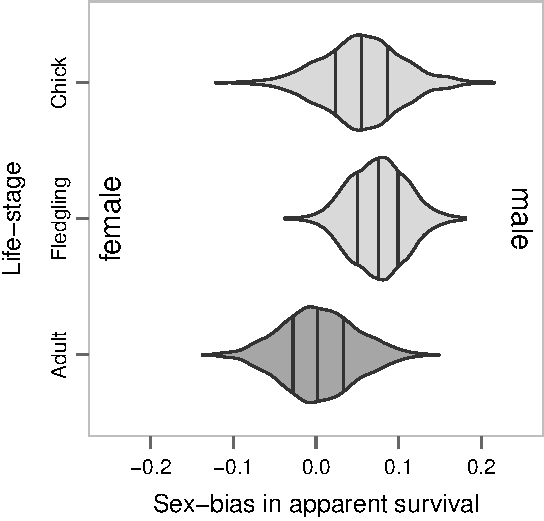
\includegraphics{Ceuta_ASR_Matrix_Modeling_files/figure-latex/unnamed-chunk-50-1} \end{center}

\textbf{Adult sex ratio distribution}

calculate the confidence interval, mean, and median of the ASR
bootstraps

\begin{Shaded}
\begin{Highlighting}[]
\NormalTok{CI <-}\StringTok{ }\FloatTok{0.95}
\NormalTok{ASR_boot_95CI <-}\StringTok{ }\NormalTok{stats::}\KeywordTok{quantile}\NormalTok{(ASR_boot$ASR_boot, }\KeywordTok{c}\NormalTok{((}\DecValTok{1} \NormalTok{-}\StringTok{ }\NormalTok{CI)/}\DecValTok{2}\NormalTok{, }\DecValTok{1} \NormalTok{-}\StringTok{ }\NormalTok{(}\DecValTok{1} \NormalTok{-}\StringTok{ }\NormalTok{CI)/}\DecValTok{2}\NormalTok{), }\DataTypeTok{na.rm =} \OtherTok{TRUE}\NormalTok{)}
\NormalTok{ASR_boot_mean <-}\StringTok{ }\KeywordTok{mean}\NormalTok{(ASR_boot$ASR_boot)}
\NormalTok{ASR_boot_median <-}\StringTok{ }\KeywordTok{median}\NormalTok{(ASR_boot$ASR_boot)}
\end{Highlighting}
\end{Shaded}

consolidate the results

\begin{Shaded}
\begin{Highlighting}[]
\NormalTok{ASR_boot_summary <-}\StringTok{ }\KeywordTok{as.data.frame}\NormalTok{(}\KeywordTok{cbind}\NormalTok{(ASR_boot_95CI[}\DecValTok{1}\NormalTok{], ASR_boot_95CI[}\DecValTok{2}\NormalTok{], }
                                        \NormalTok{ASR_boot_mean, ASR_boot_median))}
\KeywordTok{rownames}\NormalTok{(ASR_boot_summary) <-}\StringTok{ }\OtherTok{NULL}
\KeywordTok{colnames}\NormalTok{(ASR_boot_summary) <-}\StringTok{ }\KeywordTok{c}\NormalTok{(}\StringTok{"lcl"}\NormalTok{, }\StringTok{"ucl"}\NormalTok{, }\StringTok{"mean"}\NormalTok{, }\StringTok{"median"}\NormalTok{)}
\end{Highlighting}
\end{Shaded}

We visualized the bootstrapped results of adult sex ratio with a
histogram. The horizontal black bar above the distribution illustrates
the 95\% confidence interval of the 1000 iterations.

\begin{Shaded}
\begin{Highlighting}[]
\NormalTok{ggplot2::}\KeywordTok{ggplot}\NormalTok{() +}
\StringTok{          }\KeywordTok{annotate}\NormalTok{(}\StringTok{"rect"}\NormalTok{, }\DataTypeTok{xmin=}\NormalTok{-}\OtherTok{Inf}\NormalTok{, }\DataTypeTok{xmax=}\FloatTok{0.5}\NormalTok{, }\DataTypeTok{ymin=}\NormalTok{-}\OtherTok{Inf}\NormalTok{, }\DataTypeTok{ymax=}\OtherTok{Inf}\NormalTok{, }\DataTypeTok{alpha=}\FloatTok{0.6}\NormalTok{,}
                   \DataTypeTok{fill=}\KeywordTok{brewer.pal}\NormalTok{(}\DecValTok{8}\NormalTok{, }\StringTok{"Dark2"}\NormalTok{)[}\KeywordTok{c}\NormalTok{(}\DecValTok{2}\NormalTok{)]) +}
\StringTok{          }\KeywordTok{annotate}\NormalTok{(}\StringTok{"rect"}\NormalTok{, }\DataTypeTok{xmin=}\FloatTok{0.5}\NormalTok{, }\DataTypeTok{xmax=}\OtherTok{Inf}\NormalTok{, }\DataTypeTok{ymin=}\NormalTok{-}\OtherTok{Inf}\NormalTok{, }\DataTypeTok{ymax=}\OtherTok{Inf}\NormalTok{, }\DataTypeTok{alpha=}\FloatTok{0.6}\NormalTok{,}
                   \DataTypeTok{fill=}\KeywordTok{brewer.pal}\NormalTok{(}\DecValTok{8}\NormalTok{, }\StringTok{"Dark2"}\NormalTok{)[}\KeywordTok{c}\NormalTok{(}\DecValTok{1}\NormalTok{)]) +}
\StringTok{          }\KeywordTok{annotate}\NormalTok{(}\StringTok{"text"}\NormalTok{, }\DataTypeTok{x =} \KeywordTok{c}\NormalTok{(-}\OtherTok{Inf}\NormalTok{,}\OtherTok{Inf}\NormalTok{), }\DataTypeTok{y =} \KeywordTok{c}\NormalTok{(}\DecValTok{95}\NormalTok{, }\DecValTok{95}\NormalTok{),}
                   \DataTypeTok{label =} \KeywordTok{c}\NormalTok{(}\StringTok{"female"}\NormalTok{, }\StringTok{"male"}\NormalTok{), }\DataTypeTok{size =} \DecValTok{5}\NormalTok{,}
                   \DataTypeTok{vjust =} \KeywordTok{c}\NormalTok{(}\FloatTok{1.5}\NormalTok{,}\FloatTok{1.5}\NormalTok{), }\DataTypeTok{hjust =} \KeywordTok{c}\NormalTok{(}\DecValTok{0}\NormalTok{,}\DecValTok{0}\NormalTok{), }\DataTypeTok{angle =} \KeywordTok{c}\NormalTok{(}\DecValTok{90}\NormalTok{, }\DecValTok{270}\NormalTok{)) +}
\StringTok{          }\KeywordTok{geom_histogram}\NormalTok{(}\DataTypeTok{binwidth =} \FloatTok{0.02}\NormalTok{, }\DataTypeTok{data =} \NormalTok{ASR_boot, }\KeywordTok{aes}\NormalTok{(}\DataTypeTok{x =} \NormalTok{ASR_boot)) +}
\StringTok{          }\KeywordTok{geom_errorbarh}\NormalTok{(}\DataTypeTok{data =} \NormalTok{ASR_boot_summary, }
                         \KeywordTok{aes}\NormalTok{(}\DataTypeTok{y =} \DecValTok{155}\NormalTok{, }\DataTypeTok{x =} \NormalTok{lcl, }\DataTypeTok{xmin =} \NormalTok{lcl, }\DataTypeTok{xmax =} \NormalTok{ucl), }
                         \DataTypeTok{color =} \StringTok{"black"}\NormalTok{, }\DataTypeTok{size =} \FloatTok{0.8}\NormalTok{, }\DataTypeTok{linetype =} \StringTok{"solid"}\NormalTok{) +}
\StringTok{          }\KeywordTok{theme_bw}\NormalTok{() +}
\StringTok{          }\KeywordTok{theme}\NormalTok{(}\DataTypeTok{legend.position=}\StringTok{"none"}\NormalTok{,}
                \DataTypeTok{legend.position =} \KeywordTok{c}\NormalTok{(}\DecValTok{0}\NormalTok{, }\DecValTok{1}\NormalTok{), }
                \DataTypeTok{legend.justification =} \KeywordTok{c}\NormalTok{(}\DecValTok{0}\NormalTok{, }\DecValTok{1}\NormalTok{),}
                \DataTypeTok{legend.text=}\KeywordTok{element_text}\NormalTok{(}\DataTypeTok{size=}\DecValTok{11}\NormalTok{),}
                \DataTypeTok{legend.title=}\KeywordTok{element_blank}\NormalTok{(),}
                \DataTypeTok{legend.key.height=}\KeywordTok{unit}\NormalTok{(}\FloatTok{0.8}\NormalTok{,}\StringTok{"line"}\NormalTok{),}
                \DataTypeTok{legend.key.width=}\KeywordTok{unit}\NormalTok{(}\FloatTok{0.8}\NormalTok{,}\StringTok{"line"}\NormalTok{),}
                \DataTypeTok{legend.background =} \KeywordTok{element_rect}\NormalTok{(}\DataTypeTok{fill=}\OtherTok{NA}\NormalTok{),}
                \DataTypeTok{axis.title.x =} \KeywordTok{element_text}\NormalTok{(}\DataTypeTok{size=}\DecValTok{12}\NormalTok{, }\DataTypeTok{margin =} \KeywordTok{margin}\NormalTok{(}\DecValTok{10}\NormalTok{, }\DecValTok{0}\NormalTok{, }\DecValTok{0}\NormalTok{, }\DecValTok{0}\NormalTok{)),}
                \DataTypeTok{axis.text.x  =} \KeywordTok{element_text}\NormalTok{(}\DataTypeTok{size=}\DecValTok{10}\NormalTok{, }\DataTypeTok{margin =} \KeywordTok{margin}\NormalTok{(}\DecValTok{5}\NormalTok{, }\DecValTok{0}\NormalTok{, }\DecValTok{0}\NormalTok{, }\DecValTok{0}\NormalTok{)), }
                \DataTypeTok{axis.title.y =} \KeywordTok{element_text}\NormalTok{(}\DataTypeTok{size=}\DecValTok{12}\NormalTok{, }\DataTypeTok{margin =} \KeywordTok{margin}\NormalTok{(}\DecValTok{0}\NormalTok{, }\DecValTok{15}\NormalTok{, }\DecValTok{0}\NormalTok{, }\DecValTok{0}\NormalTok{)),}
                \DataTypeTok{axis.text.y  =} \KeywordTok{element_text}\NormalTok{(}\DataTypeTok{size=}\DecValTok{10}\NormalTok{, }\DataTypeTok{angle =} \DecValTok{90}\NormalTok{, }\DataTypeTok{hjust =} \FloatTok{0.5}\NormalTok{, }
                                            \DataTypeTok{margin =} \KeywordTok{margin}\NormalTok{(}\DecValTok{0}\NormalTok{, }\DecValTok{5}\NormalTok{, }\DecValTok{0}\NormalTok{, }\DecValTok{0}\NormalTok{), }\DataTypeTok{color =} \StringTok{"white"}\NormalTok{),}
                \DataTypeTok{axis.ticks.y =} \KeywordTok{element_line}\NormalTok{(}\DataTypeTok{size =} \FloatTok{0.5}\NormalTok{, }\DataTypeTok{colour =} \StringTok{"white"}\NormalTok{),}
                \DataTypeTok{axis.ticks.x =} \KeywordTok{element_line}\NormalTok{(}\DataTypeTok{size =} \FloatTok{0.5}\NormalTok{, }\DataTypeTok{colour =} \StringTok{"grey40"}\NormalTok{),}
                \DataTypeTok{axis.ticks.length =} \KeywordTok{unit}\NormalTok{(}\FloatTok{0.2}\NormalTok{, }\StringTok{"cm"}\NormalTok{),}
                \DataTypeTok{panel.grid.major =} \KeywordTok{element_blank}\NormalTok{(),}
                \DataTypeTok{panel.grid.minor =} \KeywordTok{element_blank}\NormalTok{(),}
                \DataTypeTok{panel.border =} \KeywordTok{element_rect}\NormalTok{(}\DataTypeTok{linetype =} \StringTok{"solid"}\NormalTok{, }\DataTypeTok{colour =} \StringTok{"grey"}\NormalTok{),}
                \DataTypeTok{plot.margin =} \KeywordTok{unit}\NormalTok{(}\KeywordTok{c}\NormalTok{(}\DecValTok{1}\NormalTok{,}\FloatTok{0.5}\NormalTok{,}\FloatTok{0.5}\NormalTok{,}\FloatTok{0.5}\NormalTok{), }\StringTok{"cm"}\NormalTok{),}
                \DataTypeTok{strip.background =} \KeywordTok{element_blank}\NormalTok{(), }
                \DataTypeTok{strip.text =} \KeywordTok{element_blank}\NormalTok{(),}
                \DataTypeTok{panel.margin =} \KeywordTok{unit}\NormalTok{(}\FloatTok{0.75}\NormalTok{, }\StringTok{"lines"}\NormalTok{)) +}
\StringTok{          }\KeywordTok{ylab}\NormalTok{(}\StringTok{"Frequency"}\NormalTok{) +}
\StringTok{          }\KeywordTok{xlab}\NormalTok{(}\StringTok{"Adult sex ratio (proportion male)"}\NormalTok{) +}
\StringTok{          }\KeywordTok{scale_x_continuous}\NormalTok{(}\DataTypeTok{limits =} \KeywordTok{c}\NormalTok{(}\FloatTok{0.0}\NormalTok{, }\DecValTok{1}\NormalTok{)) +}
\StringTok{          }\KeywordTok{scale_y_continuous}\NormalTok{(}\DataTypeTok{limits =} \KeywordTok{c}\NormalTok{(}\DecValTok{0}\NormalTok{, }\DecValTok{160}\NormalTok{))}
\end{Highlighting}
\end{Shaded}

\begin{center}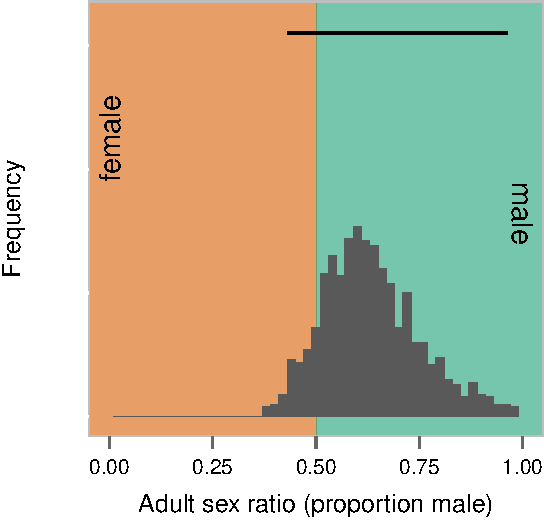
\includegraphics{Ceuta_ASR_Matrix_Modeling_files/figure-latex/unnamed-chunk-53-1} \end{center}

\textbf{AIC model selection summary (panels in Supplementary Material
Figure 1)}

To illustrate the mark-recapture model selection going on during the
bootstrap, we summarized AIC statistics for each model included in the
survival analysis and visualized with ranked boxplots

First, wrangle the bootstrap AIC table output

\begin{Shaded}
\begin{Highlighting}[]
\CommentTok{# define the model number}
\NormalTok{chick_AIC_tables$model_number <-}\StringTok{ }\KeywordTok{as.numeric}\NormalTok{(chick_AIC_tables$model)}

\NormalTok{fldg_ad_AIC_tables$model_number <-}\StringTok{ }\KeywordTok{as.numeric}\NormalTok{(fldg_ad_AIC_tables$model)}

\CommentTok{# summarize the average AIC stats for each candidate model across all 1000 iterations}
\NormalTok{chick_AIC_tables_summary <-}\StringTok{ }
\StringTok{  }\NormalTok{chick_AIC_tables %>%}
\StringTok{  }\NormalTok{dplyr::}\KeywordTok{group_by}\NormalTok{(model) %>%}
\StringTok{  }\NormalTok{dplyr::}\KeywordTok{summarise}\NormalTok{(}\DataTypeTok{avg_Delta =} \KeywordTok{mean}\NormalTok{(DeltaAICc),}
            \DataTypeTok{IQR_Delta =} \KeywordTok{IQR}\NormalTok{(DeltaAICc),}
            \DataTypeTok{avg_Weight =} \KeywordTok{mean}\NormalTok{(weight),}
            \DataTypeTok{IQR_Weight =} \KeywordTok{IQR}\NormalTok{(weight))}

\NormalTok{fldg_ad_AIC_tables_summary <-}\StringTok{ }
\StringTok{  }\NormalTok{fldg_ad_AIC_tables %>%}
\StringTok{  }\NormalTok{dplyr::}\KeywordTok{group_by}\NormalTok{(model) %>%}
\StringTok{  }\NormalTok{dplyr::}\KeywordTok{summarise}\NormalTok{(}\DataTypeTok{avg_Delta =} \KeywordTok{mean}\NormalTok{(DeltaAICc),}
            \DataTypeTok{IQR_Delta =} \KeywordTok{IQR}\NormalTok{(DeltaAICc),}
            \DataTypeTok{avg_Weight =} \KeywordTok{mean}\NormalTok{(weight),}
            \DataTypeTok{IQR_Weight =} \KeywordTok{IQR}\NormalTok{(weight))}

\CommentTok{# rank the output by delta AIC and determine model number}
\NormalTok{chick_AIC_tables_summary <-}\StringTok{ }\NormalTok{dplyr::}\KeywordTok{arrange}\NormalTok{(chick_AIC_tables_summary, avg_Delta)}
\NormalTok{chick_AIC_tables_summary$model_number <-}\StringTok{ }\KeywordTok{as.numeric}\NormalTok{(chick_AIC_tables_summary$model)}

\NormalTok{fldg_ad_AIC_tables_summary <-}\StringTok{ }\NormalTok{dplyr::}\KeywordTok{arrange}\NormalTok{(fldg_ad_AIC_tables_summary, avg_Delta)}
\NormalTok{fldg_ad_AIC_tables_summary$model_number <-}\StringTok{ }\KeywordTok{as.numeric}\NormalTok{(fldg_ad_AIC_tables_summary$model)}

\CommentTok{# merge the two datasets for plotting}
\NormalTok{chick_AIC_tables <-}\StringTok{ }
\StringTok{  }\NormalTok{dplyr::}\KeywordTok{left_join}\NormalTok{(chick_AIC_tables_summary, chick_AIC_tables, }\DataTypeTok{by =} \StringTok{"model_number"}\NormalTok{)}

\NormalTok{fldg_ad_AIC_tables <-}\StringTok{ }
\StringTok{  }\NormalTok{dplyr::}\KeywordTok{left_join}\NormalTok{(fldg_ad_AIC_tables_summary, fldg_ad_AIC_tables, }\DataTypeTok{by =} \StringTok{"model_number"}\NormalTok{)}

\CommentTok{# extract the model structure explaining resighting probability}
\NormalTok{chick_AIC_tables$p <-}\StringTok{ }
\StringTok{  }\KeywordTok{factor}\NormalTok{(chick_AIC_tables$p, }
         \DataTypeTok{levels =} \KeywordTok{str_sub}\NormalTok{(}\KeywordTok{as.character}\NormalTok{(chick_AIC_tables_summary$model), }
                          \DataTypeTok{start =} \DecValTok{24}\NormalTok{, }\DataTypeTok{end =} \KeywordTok{str_length}\NormalTok{(chick_AIC_tables_summary$model)-}\DecValTok{1}\NormalTok{))}

\NormalTok{fldg_ad_AIC_tables$p <-}\StringTok{ }
\StringTok{  }\KeywordTok{factor}\NormalTok{(fldg_ad_AIC_tables$p,}
         \DataTypeTok{levels =} \KeywordTok{str_sub}\NormalTok{(}\KeywordTok{as.character}\NormalTok{(fldg_ad_AIC_tables_summary$model), }
                        \DataTypeTok{start =} \DecValTok{18}\NormalTok{, }\DataTypeTok{end =} \KeywordTok{str_length}\NormalTok{(fldg_ad_AIC_tables_summary$model)-}\DecValTok{1}\NormalTok{))}
\end{Highlighting}
\end{Shaded}

plot the overall model ranks of the chick survival anlaysis based on
Delta AIC

\begin{Shaded}
\begin{Highlighting}[]
\NormalTok{ggplot2::}\KeywordTok{ggplot}\NormalTok{(}\KeywordTok{aes}\NormalTok{(}\DataTypeTok{y =} \NormalTok{DeltaAICc, }\DataTypeTok{x =} \NormalTok{p), }\DataTypeTok{data =} \NormalTok{chick_AIC_tables) +}\StringTok{ }
\StringTok{          }\KeywordTok{theme_bw}\NormalTok{() +}
\StringTok{          }\KeywordTok{geom_boxplot}\NormalTok{(}\DataTypeTok{width =} \FloatTok{0.3}\NormalTok{, }\DataTypeTok{fill =} \StringTok{"grey70"}\NormalTok{, }\DataTypeTok{outlier.size =} \FloatTok{0.5}\NormalTok{) +}
\StringTok{          }\KeywordTok{theme}\NormalTok{(}\DataTypeTok{legend.position =} \StringTok{"none"}\NormalTok{,}
                \DataTypeTok{axis.title.x =} \KeywordTok{element_blank}\NormalTok{(),}
                \DataTypeTok{axis.text.x  =} \KeywordTok{element_text}\NormalTok{(}\DataTypeTok{size=}\DecValTok{10}\NormalTok{, }\DataTypeTok{angle =} \DecValTok{45}\NormalTok{, }\DataTypeTok{hjust =} \DecValTok{1}\NormalTok{), }
                \DataTypeTok{axis.title.y =} \KeywordTok{element_text}\NormalTok{(}\DataTypeTok{size=}\DecValTok{12}\NormalTok{, }\DataTypeTok{margin =} \KeywordTok{margin}\NormalTok{(}\DecValTok{0}\NormalTok{, }\DecValTok{15}\NormalTok{, }\DecValTok{0}\NormalTok{, }\DecValTok{0}\NormalTok{)),}
                \DataTypeTok{axis.text.y  =} \KeywordTok{element_text}\NormalTok{(}\DataTypeTok{size=}\DecValTok{10}\NormalTok{),}
                \DataTypeTok{panel.grid.major =} \KeywordTok{element_blank}\NormalTok{(),}
                \DataTypeTok{panel.grid.minor =} \KeywordTok{element_blank}\NormalTok{(),}
                \DataTypeTok{axis.ticks.y =} \KeywordTok{element_line}\NormalTok{(}\DataTypeTok{size =} \FloatTok{0.5}\NormalTok{, }\DataTypeTok{colour =} \StringTok{"grey40"}\NormalTok{),}
                \DataTypeTok{axis.ticks.length =} \KeywordTok{unit}\NormalTok{(}\FloatTok{0.2}\NormalTok{, }\StringTok{"cm"}\NormalTok{),}
                \DataTypeTok{axis.ticks.x =} \KeywordTok{element_line}\NormalTok{(}\DataTypeTok{size =} \FloatTok{0.5}\NormalTok{, }\DataTypeTok{colour =} \StringTok{"grey40"}\NormalTok{),}
                \DataTypeTok{plot.margin =} \KeywordTok{unit}\NormalTok{(}\KeywordTok{c}\NormalTok{(}\FloatTok{0.5}\NormalTok{,}\FloatTok{0.5}\NormalTok{,}\FloatTok{0.5}\NormalTok{,}\FloatTok{3.0}\NormalTok{), }\StringTok{"cm"}\NormalTok{),}
                \DataTypeTok{panel.margin =} \KeywordTok{unit}\NormalTok{(}\FloatTok{0.75}\NormalTok{, }\StringTok{"lines"}\NormalTok{),}
                \DataTypeTok{strip.background =} \KeywordTok{element_blank}\NormalTok{(), }
                \DataTypeTok{strip.text =} \KeywordTok{element_blank}\NormalTok{()) +}
\StringTok{          }\KeywordTok{scale_y_continuous}\NormalTok{(}\DataTypeTok{limits=}\KeywordTok{c}\NormalTok{(}\DecValTok{0}\NormalTok{,}\DecValTok{50}\NormalTok{)) +}
\StringTok{          }\KeywordTok{xlab}\NormalTok{(}\StringTok{"Model"}\NormalTok{) +}\StringTok{ }
\StringTok{          }\KeywordTok{ylab}\NormalTok{(}\StringTok{"Delta AIC"}\NormalTok{) +}
\StringTok{          }\KeywordTok{ggtitle}\NormalTok{(}\StringTok{"Chick resighting model selection"}\NormalTok{)}
\end{Highlighting}
\end{Shaded}

\begin{center}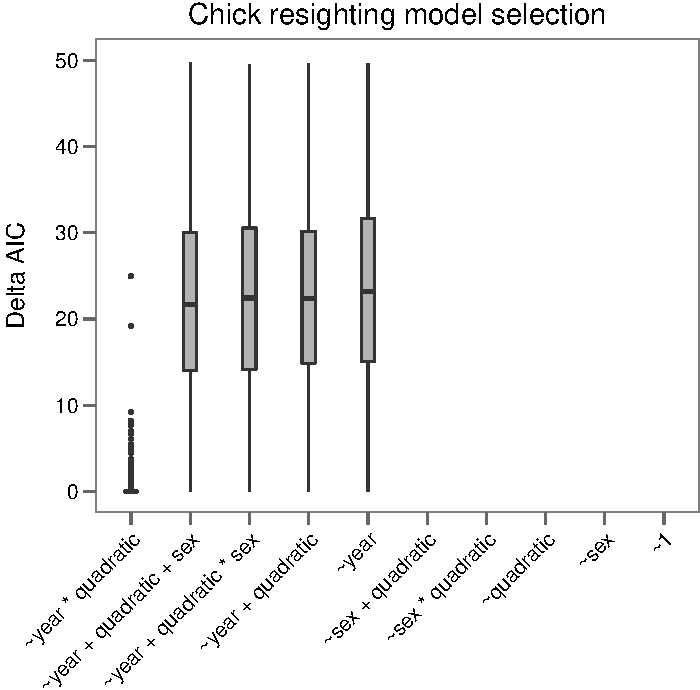
\includegraphics{Ceuta_ASR_Matrix_Modeling_files/figure-latex/unnamed-chunk-55-1} \end{center}

plot the overall model ranks of the chick survival anlaysis based on AIC
weight

\begin{Shaded}
\begin{Highlighting}[]
\NormalTok{ggplot2::}\KeywordTok{ggplot}\NormalTok{(}\KeywordTok{aes}\NormalTok{(}\DataTypeTok{y =} \NormalTok{weight, }\DataTypeTok{x =} \NormalTok{p), }\DataTypeTok{data =} \NormalTok{chick_AIC_tables) +}\StringTok{ }
\StringTok{          }\KeywordTok{theme_bw}\NormalTok{() +}
\StringTok{          }\KeywordTok{geom_boxplot}\NormalTok{(}\DataTypeTok{width =} \FloatTok{0.3}\NormalTok{, }\DataTypeTok{fill =} \StringTok{"grey70"}\NormalTok{, }\DataTypeTok{outlier.size =} \FloatTok{0.5}\NormalTok{) +}
\StringTok{          }\KeywordTok{theme}\NormalTok{(}\DataTypeTok{legend.position =} \StringTok{"none"}\NormalTok{,}
                \DataTypeTok{axis.title.x =} \KeywordTok{element_blank}\NormalTok{(),}
                \DataTypeTok{axis.text.x  =} \KeywordTok{element_text}\NormalTok{(}\DataTypeTok{size=}\DecValTok{10}\NormalTok{, }\DataTypeTok{angle =} \DecValTok{45}\NormalTok{, }\DataTypeTok{hjust =} \DecValTok{1}\NormalTok{), }
                \DataTypeTok{axis.title.y =} \KeywordTok{element_text}\NormalTok{(}\DataTypeTok{size=}\DecValTok{12}\NormalTok{, }\DataTypeTok{margin =} \KeywordTok{margin}\NormalTok{(}\DecValTok{0}\NormalTok{, }\DecValTok{15}\NormalTok{, }\DecValTok{0}\NormalTok{, }\DecValTok{0}\NormalTok{)),}
                \DataTypeTok{axis.text.y  =} \KeywordTok{element_text}\NormalTok{(}\DataTypeTok{size=}\DecValTok{10}\NormalTok{),}
                \DataTypeTok{panel.grid.major =} \KeywordTok{element_blank}\NormalTok{(),}
                \DataTypeTok{panel.grid.minor =} \KeywordTok{element_blank}\NormalTok{(),}
                \DataTypeTok{axis.ticks.y =} \KeywordTok{element_line}\NormalTok{(}\DataTypeTok{size =} \FloatTok{0.5}\NormalTok{, }\DataTypeTok{colour =} \StringTok{"grey40"}\NormalTok{),}
                \DataTypeTok{axis.ticks.length =} \KeywordTok{unit}\NormalTok{(}\FloatTok{0.2}\NormalTok{, }\StringTok{"cm"}\NormalTok{),}
                \DataTypeTok{axis.ticks.x =} \KeywordTok{element_line}\NormalTok{(}\DataTypeTok{size =} \FloatTok{0.5}\NormalTok{, }\DataTypeTok{colour =} \StringTok{"grey40"}\NormalTok{),}
                \DataTypeTok{plot.margin =} \KeywordTok{unit}\NormalTok{(}\KeywordTok{c}\NormalTok{(}\FloatTok{0.5}\NormalTok{,}\FloatTok{0.5}\NormalTok{,}\FloatTok{0.5}\NormalTok{,}\FloatTok{2.0}\NormalTok{), }\StringTok{"cm"}\NormalTok{),}
                \DataTypeTok{panel.margin =} \KeywordTok{unit}\NormalTok{(}\FloatTok{0.75}\NormalTok{, }\StringTok{"lines"}\NormalTok{),}
                \DataTypeTok{strip.background =} \KeywordTok{element_blank}\NormalTok{(), }
                \DataTypeTok{strip.text =} \KeywordTok{element_blank}\NormalTok{()) +}
\StringTok{          }\KeywordTok{scale_y_continuous}\NormalTok{(}\DataTypeTok{limits=}\KeywordTok{c}\NormalTok{(}\DecValTok{0}\NormalTok{,}\DecValTok{1}\NormalTok{)) +}
\StringTok{          }\KeywordTok{xlab}\NormalTok{(}\StringTok{"Model"}\NormalTok{) +}\StringTok{ }
\StringTok{          }\KeywordTok{ylab}\NormalTok{(}\StringTok{"AIC weight"}\NormalTok{) +}
\StringTok{          }\KeywordTok{ggtitle}\NormalTok{(}\StringTok{"Chick resighting model selection"}\NormalTok{)}
\end{Highlighting}
\end{Shaded}

\begin{center}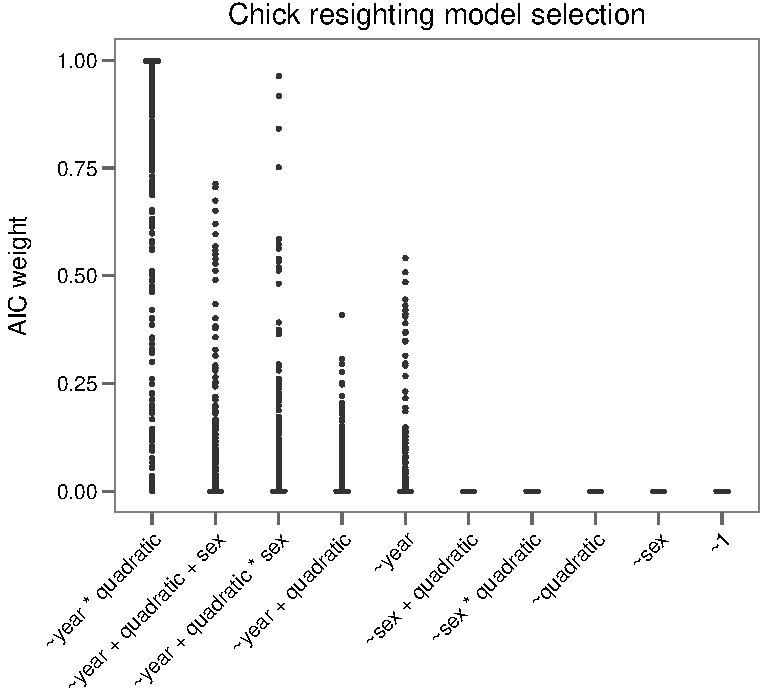
\includegraphics{Ceuta_ASR_Matrix_Modeling_files/figure-latex/unnamed-chunk-56-1} \end{center}

plot the overall model ranks of the fledgling and adult survival
anlaysis based on Delta AIC

\begin{Shaded}
\begin{Highlighting}[]
\NormalTok{ggplot2::}\KeywordTok{ggplot}\NormalTok{(}\KeywordTok{aes}\NormalTok{(}\DataTypeTok{y =} \NormalTok{DeltaAICc, }\DataTypeTok{x =} \NormalTok{p), }\DataTypeTok{data =} \NormalTok{fldg_ad_AIC_tables) +}\StringTok{ }
\StringTok{          }\KeywordTok{theme_bw}\NormalTok{() +}
\StringTok{          }\KeywordTok{geom_boxplot}\NormalTok{(}\DataTypeTok{width =} \FloatTok{0.3}\NormalTok{, }\DataTypeTok{fill =} \StringTok{"grey70"}\NormalTok{, }\DataTypeTok{outlier.size =} \FloatTok{0.5}\NormalTok{) +}
\StringTok{          }\KeywordTok{theme}\NormalTok{(}\DataTypeTok{legend.position =} \StringTok{"none"}\NormalTok{,}
                \DataTypeTok{axis.title.x =} \KeywordTok{element_blank}\NormalTok{(),}
                \DataTypeTok{axis.text.x  =} \KeywordTok{element_text}\NormalTok{(}\DataTypeTok{size=}\DecValTok{10}\NormalTok{, }\DataTypeTok{angle =} \DecValTok{45}\NormalTok{, }\DataTypeTok{hjust =} \DecValTok{1}\NormalTok{), }
                \DataTypeTok{axis.title.y =} \KeywordTok{element_text}\NormalTok{(}\DataTypeTok{size=}\DecValTok{12}\NormalTok{, }\DataTypeTok{margin =} \KeywordTok{margin}\NormalTok{(}\DecValTok{0}\NormalTok{, }\DecValTok{15}\NormalTok{, }\DecValTok{0}\NormalTok{, }\DecValTok{0}\NormalTok{)),}
                \DataTypeTok{axis.text.y  =} \KeywordTok{element_text}\NormalTok{(}\DataTypeTok{size=}\DecValTok{10}\NormalTok{),}
                \DataTypeTok{panel.grid.major =} \KeywordTok{element_blank}\NormalTok{(),}
                \DataTypeTok{panel.grid.minor =} \KeywordTok{element_blank}\NormalTok{(),}
                \DataTypeTok{axis.ticks.y =} \KeywordTok{element_line}\NormalTok{(}\DataTypeTok{size =} \FloatTok{0.5}\NormalTok{, }\DataTypeTok{colour =} \StringTok{"grey40"}\NormalTok{),}
                \DataTypeTok{axis.ticks.length =} \KeywordTok{unit}\NormalTok{(}\FloatTok{0.2}\NormalTok{, }\StringTok{"cm"}\NormalTok{),}
                \DataTypeTok{axis.ticks.x =} \KeywordTok{element_line}\NormalTok{(}\DataTypeTok{size =} \FloatTok{0.5}\NormalTok{, }\DataTypeTok{colour =} \StringTok{"grey40"}\NormalTok{),}
                \DataTypeTok{plot.margin =} \KeywordTok{unit}\NormalTok{(}\KeywordTok{c}\NormalTok{(}\FloatTok{0.5}\NormalTok{,}\FloatTok{0.5}\NormalTok{,}\FloatTok{0.5}\NormalTok{,}\FloatTok{2.0}\NormalTok{), }\StringTok{"cm"}\NormalTok{),}
                \DataTypeTok{panel.margin =} \KeywordTok{unit}\NormalTok{(}\FloatTok{0.75}\NormalTok{, }\StringTok{"lines"}\NormalTok{),}
                \DataTypeTok{strip.background =} \KeywordTok{element_blank}\NormalTok{(), }
                \DataTypeTok{strip.text =} \KeywordTok{element_blank}\NormalTok{()) +}
\StringTok{          }\KeywordTok{scale_y_continuous}\NormalTok{(}\DataTypeTok{limits=}\KeywordTok{c}\NormalTok{(}\DecValTok{0}\NormalTok{,}\DecValTok{50}\NormalTok{)) +}
\StringTok{          }\KeywordTok{xlab}\NormalTok{(}\StringTok{"Model"}\NormalTok{) +}\StringTok{ }
\StringTok{          }\KeywordTok{ylab}\NormalTok{(}\StringTok{"Delta AIC"}\NormalTok{) +}
\StringTok{          }\KeywordTok{ggtitle}\NormalTok{(}\StringTok{"Fledgling and adult resighting model selection"}\NormalTok{)}
\end{Highlighting}
\end{Shaded}

\begin{center}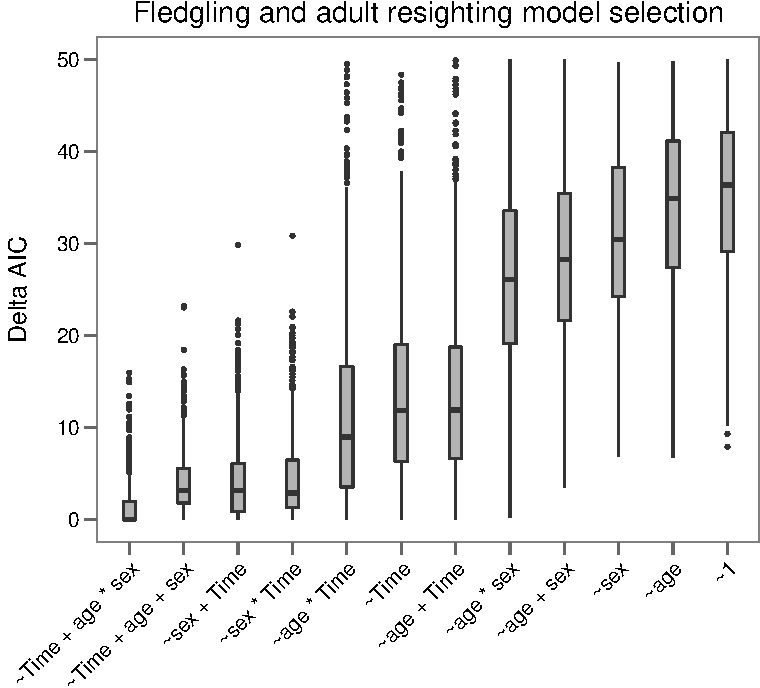
\includegraphics{Ceuta_ASR_Matrix_Modeling_files/figure-latex/unnamed-chunk-57-1} \end{center}

plot the overall model ranks of the fledgling and adult survival
anlaysis based on AIC weight

\begin{Shaded}
\begin{Highlighting}[]
\NormalTok{ggplot2::}\KeywordTok{ggplot}\NormalTok{(}\KeywordTok{aes}\NormalTok{(}\DataTypeTok{y =} \NormalTok{weight, }\DataTypeTok{x =} \NormalTok{p), }\DataTypeTok{data =} \NormalTok{fldg_ad_AIC_tables) +}\StringTok{ }
\StringTok{          }\KeywordTok{theme_bw}\NormalTok{() +}
\StringTok{          }\KeywordTok{geom_boxplot}\NormalTok{(}\DataTypeTok{width =} \FloatTok{0.3}\NormalTok{, }\DataTypeTok{fill =} \StringTok{"grey70"}\NormalTok{, }\DataTypeTok{outlier.size =} \FloatTok{0.5}\NormalTok{) +}
\StringTok{          }\KeywordTok{theme}\NormalTok{(}\DataTypeTok{legend.position =} \StringTok{"none"}\NormalTok{,}
                \DataTypeTok{axis.title.x =} \KeywordTok{element_blank}\NormalTok{(),}
                \DataTypeTok{axis.text.x  =} \KeywordTok{element_text}\NormalTok{(}\DataTypeTok{size=}\DecValTok{10}\NormalTok{, }\DataTypeTok{angle =} \DecValTok{45}\NormalTok{, }\DataTypeTok{hjust =} \DecValTok{1}\NormalTok{), }
                \DataTypeTok{axis.title.y =} \KeywordTok{element_text}\NormalTok{(}\DataTypeTok{size=}\DecValTok{12}\NormalTok{, }\DataTypeTok{margin =} \KeywordTok{margin}\NormalTok{(}\DecValTok{0}\NormalTok{, }\DecValTok{15}\NormalTok{, }\DecValTok{0}\NormalTok{, }\DecValTok{0}\NormalTok{)),}
                \DataTypeTok{axis.text.y  =} \KeywordTok{element_text}\NormalTok{(}\DataTypeTok{size=}\DecValTok{10}\NormalTok{),}
                \DataTypeTok{panel.grid.major =} \KeywordTok{element_blank}\NormalTok{(),}
                \DataTypeTok{panel.grid.minor =} \KeywordTok{element_blank}\NormalTok{(),}
                \DataTypeTok{axis.ticks.y =} \KeywordTok{element_line}\NormalTok{(}\DataTypeTok{size =} \FloatTok{0.5}\NormalTok{, }\DataTypeTok{colour =} \StringTok{"grey40"}\NormalTok{),}
                \DataTypeTok{axis.ticks.length =} \KeywordTok{unit}\NormalTok{(}\FloatTok{0.2}\NormalTok{, }\StringTok{"cm"}\NormalTok{),}
                \DataTypeTok{axis.ticks.x =} \KeywordTok{element_line}\NormalTok{(}\DataTypeTok{size =} \FloatTok{0.5}\NormalTok{, }\DataTypeTok{colour =} \StringTok{"grey40"}\NormalTok{),}
                \DataTypeTok{plot.margin =} \KeywordTok{unit}\NormalTok{(}\KeywordTok{c}\NormalTok{(}\FloatTok{0.5}\NormalTok{,}\FloatTok{0.5}\NormalTok{,}\FloatTok{0.5}\NormalTok{,}\FloatTok{2.0}\NormalTok{), }\StringTok{"cm"}\NormalTok{),}
                \DataTypeTok{panel.margin =} \KeywordTok{unit}\NormalTok{(}\FloatTok{0.75}\NormalTok{, }\StringTok{"lines"}\NormalTok{),}
                \DataTypeTok{strip.background =} \KeywordTok{element_blank}\NormalTok{(), }
                \DataTypeTok{strip.text =} \KeywordTok{element_blank}\NormalTok{(),}
                \DataTypeTok{plot.background =} \KeywordTok{element_rect}\NormalTok{(}\DataTypeTok{fill =} \StringTok{"transparent"}\NormalTok{,}\DataTypeTok{colour =} \OtherTok{NA}\NormalTok{)) +}
\StringTok{          }\KeywordTok{scale_y_continuous}\NormalTok{(}\DataTypeTok{limits=}\KeywordTok{c}\NormalTok{(}\DecValTok{0}\NormalTok{,}\DecValTok{1}\NormalTok{)) +}
\StringTok{          }\KeywordTok{xlab}\NormalTok{(}\StringTok{"Model"}\NormalTok{) +}\StringTok{ }
\StringTok{          }\KeywordTok{ylab}\NormalTok{(}\StringTok{"AIC weight"}\NormalTok{) +}
\StringTok{          }\KeywordTok{ggtitle}\NormalTok{(}\StringTok{"Fledgling and adult resighting model selection"}\NormalTok{)}
\end{Highlighting}
\end{Shaded}

\begin{center}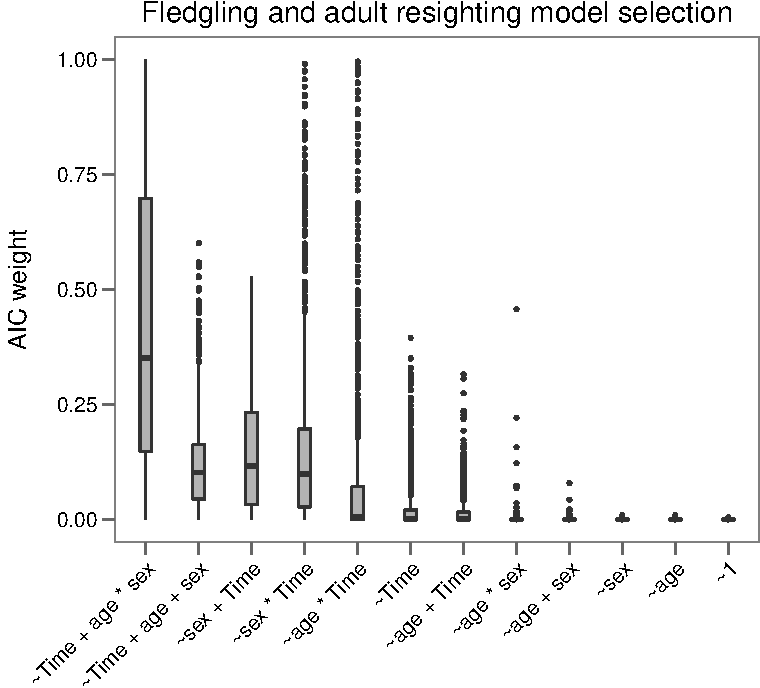
\includegraphics{Ceuta_ASR_Matrix_Modeling_files/figure-latex/unnamed-chunk-58-1} \end{center}

\begin{center}\rule{0.5\linewidth}{\linethickness}\end{center}

\subsection{Life table response
experiment}\label{life-table-response-experiment}

Perturbation analyses provide important information about the relative
contribution that each component of a matrix model has on the response,
in our case ASR. To assess how influential a sex-bias in each of the
three life-stages is on ASR dynamics, we employed a life-table response
experiment (LTRE). In essence, the LTRE compares the response of a
``control'' matrix to that of a ``treatment'' matrix and assesses the
relative contribution that model components have on the effect size of
the treatment.

The following two functions need to be specified first. Note: these were
modified from the \textbf{popbio} R package by Chris Stubben, Brook
Milligan, and Patrick Nantel. Modifications were made so that the
response was ASR rather than lambda.

\textbf{ASR\_analysis()} determines the stable-stage distribution from a
matrix (A) and then calculates the ASR as the proportion of the adults
in that distribution that are male.

\begin{Shaded}
\begin{Highlighting}[]
\NormalTok{ASR_analysis <-}\StringTok{ }
\StringTok{  }\NormalTok{function (A, }\DataTypeTok{zero =} \OtherTok{TRUE}\NormalTok{) }
    \NormalTok{\{}
    
    \CommentTok{# makes list of the eigen values and eigen vectors of A}
    \NormalTok{ev <-}\StringTok{ }\KeywordTok{eigen}\NormalTok{(A) }
    
    \CommentTok{# index of dominant eigen value}
    \NormalTok{lmax <-}\StringTok{ }\KeywordTok{which.max}\NormalTok{(}\KeywordTok{Re}\NormalTok{(ev$values)) }
    
    \CommentTok{# Eigen vectors}
    \NormalTok{W <-}\StringTok{ }\NormalTok{ev$vectors }
    
    \CommentTok{# dominant eigen vector}
    \NormalTok{w <-}\StringTok{ }\KeywordTok{abs}\NormalTok{(}\KeywordTok{Re}\NormalTok{(W[, lmax])) }
    
    \CommentTok{# stable stage distribution}
    \NormalTok{stable.stage =}\StringTok{ }\NormalTok{w /}\StringTok{ }\KeywordTok{sum}\NormalTok{(w) }
    
    \CommentTok{# ASR}
    \NormalTok{ASR <-}\StringTok{ }\NormalTok{stable.stage[}\DecValTok{4}\NormalTok{] /}\StringTok{ }\NormalTok{(stable.stage[}\DecValTok{2}\NormalTok{] +}\StringTok{ }\NormalTok{stable.stage[}\DecValTok{4}\NormalTok{]) }
    
    \CommentTok{# check if possible to proceed}
    \NormalTok{V <-}\StringTok{ }\KeywordTok{try}\NormalTok{(}\KeywordTok{Conj}\NormalTok{(}\KeywordTok{solve}\NormalTok{(W)), }\DataTypeTok{silent =} \OtherTok{TRUE}\NormalTok{)}
    \NormalTok{if (}\KeywordTok{class}\NormalTok{(V) ==}\StringTok{ "try-error"}\NormalTok{) \{}
      \NormalTok{ASR.analysis <-}\StringTok{ }\KeywordTok{list}\NormalTok{(}\DataTypeTok{ASR =} \NormalTok{ASR, }\DataTypeTok{stable.stage =} \NormalTok{stable.stage, }
                           \DataTypeTok{sensitivities =} \NormalTok{A *}\StringTok{ }\OtherTok{NA}\NormalTok{, }\DataTypeTok{elasticities =} \NormalTok{A *}\StringTok{ }\OtherTok{NA}\NormalTok{)}
    \NormalTok{\}}
  \NormalTok{else \{}
    
    \CommentTok{# solve matrix}
    \NormalTok{v <-}\StringTok{ }\KeywordTok{abs}\NormalTok{(}\KeywordTok{Re}\NormalTok{(V[lmax, ])) }
    
    \CommentTok{# outer product of v and w}
    \NormalTok{s <-}\StringTok{ }\NormalTok{v %o%}\StringTok{ }\NormalTok{w }
    \NormalTok{if (zero) \{}
      \NormalTok{s[A ==}\StringTok{ }\DecValTok{0}\NormalTok{] <-}\StringTok{ }\DecValTok{0}
    \NormalTok{\}}
    
     \CommentTok{# calculate elasticities}
    \NormalTok{e <-}\StringTok{ }\NormalTok{s *}\StringTok{ }\NormalTok{A/ASR}
    
    \CommentTok{# get vital rate names}
    \NormalTok{x <-}\StringTok{ }\KeywordTok{dimnames}\NormalTok{(A) }
    
    \CommentTok{# assign vital rate names to s}
    \KeywordTok{dimnames}\NormalTok{(s) <-}\StringTok{ }\NormalTok{x }
    \KeywordTok{names}\NormalTok{(w) <-}\StringTok{ }\NormalTok{x[[}\DecValTok{1}\NormalTok{]]}
    \KeywordTok{names}\NormalTok{(v) <-}\StringTok{ }\NormalTok{x[[}\DecValTok{1}\NormalTok{]]}
    
    \CommentTok{# output a list containing the ASR, SSD, sensitivites, and elasticities}
    \NormalTok{ASR.analysis <-}\StringTok{ }\KeywordTok{list}\NormalTok{(}\DataTypeTok{ASR =} \NormalTok{ASR, }\DataTypeTok{stable.stage =} \NormalTok{stable.stage, }
                         \DataTypeTok{sensitivities =} \NormalTok{s, }\DataTypeTok{elasticities =} \NormalTok{e)}
  \NormalTok{\}}
  \NormalTok{ASR.analysis}
\NormalTok{\}}
\end{Highlighting}
\end{Shaded}

\textbf{ASR\_perturbation()} determines the lower-level sensitivites of
each matrix element then runs the LTRE analysis.

\begin{Shaded}
\begin{Highlighting}[]
\NormalTok{ASR_perturbation <-}\StringTok{ }
\StringTok{  }\NormalTok{function (elements, VR_list, freq_dep_ASR) }
  \NormalTok{\{}
    
      \CommentTok{# list of parameters in the treatment matrix}
      \CommentTok{# this contains the observed paramters based on previous analyses}
      \NormalTok{treatment_matrix <-}\StringTok{ }\KeywordTok{list}\NormalTok{(}
        \DataTypeTok{F_Chk_survl =} \NormalTok{VR_list$F_Chk_survl,}
        \DataTypeTok{F_Fdg_survl =} \NormalTok{VR_list$F_Fdg_survl,}
        \DataTypeTok{F_Adt_survl =} \NormalTok{VR_list$F_Adt_survl,}
        \DataTypeTok{M_Chk_survl =} \NormalTok{VR_list$M_Chk_survl,}
        \DataTypeTok{M_Fdg_survl =} \NormalTok{VR_list$M_Fdg_survl,}
        \DataTypeTok{M_Adt_survl =} \NormalTok{VR_list$M_Adt_survl,}
        \DataTypeTok{RF =} \NormalTok{VR_list$RF,}
        \DataTypeTok{HSR =} \NormalTok{VR_list$HSR)}
      
      \CommentTok{# list of parameters in the control matrix}
      \CommentTok{# this contains parameters with no sex-differences}
      \NormalTok{control_matrix <-}\StringTok{ }\KeywordTok{list}\NormalTok{(}
        \DataTypeTok{F_Chk_survl =} \NormalTok{VR_list$M_Chk_survl,}
        \DataTypeTok{F_Fdg_survl =} \NormalTok{VR_list$M_Fdg_survl,}
        \DataTypeTok{F_Adt_survl =} \NormalTok{VR_list$M_Adt_survl,}
        \DataTypeTok{M_Chk_survl =} \NormalTok{VR_list$M_Chk_survl,}
        \DataTypeTok{M_Fdg_survl =} \NormalTok{VR_list$M_Fdg_survl,}
        \DataTypeTok{M_Adt_survl =} \NormalTok{VR_list$M_Adt_survl,}
        \DataTypeTok{RF =} \NormalTok{VR_list$RF,}
        \DataTypeTok{HSR =} \FloatTok{0.5}\NormalTok{)}
      
      \CommentTok{# list of parameters in the M-prime matrix}
      \CommentTok{# this contains the average difference between each parameter}
      \NormalTok{M_prime_matrix <-}\StringTok{ }\KeywordTok{list}\NormalTok{(}
        \DataTypeTok{F_Chk_survl =} \NormalTok{(treatment_matrix$F_Chk_survl +}\StringTok{ }\NormalTok{control_matrix$F_Chk_survl)/}\DecValTok{2}\NormalTok{,}
        \DataTypeTok{F_Fdg_survl =} \NormalTok{(treatment_matrix$F_Fdg_survl +}\StringTok{ }\NormalTok{control_matrix$F_Fdg_survl)/}\DecValTok{2}\NormalTok{,}
        \DataTypeTok{F_Adt_survl =} \NormalTok{(treatment_matrix$F_Adt_survl +}\StringTok{ }\NormalTok{control_matrix$F_Adt_survl)/}\DecValTok{2}\NormalTok{,}
        \DataTypeTok{M_Chk_survl =} \NormalTok{(treatment_matrix$M_Chk_survl +}\StringTok{ }\NormalTok{control_matrix$M_Chk_survl)/}\DecValTok{2}\NormalTok{,}
        \DataTypeTok{M_Fdg_survl =} \NormalTok{(treatment_matrix$M_Fdg_survl +}\StringTok{ }\NormalTok{control_matrix$M_Fdg_survl)/}\DecValTok{2}\NormalTok{,}
        \DataTypeTok{M_Adt_survl =} \NormalTok{(treatment_matrix$M_Adt_survl +}\StringTok{ }\NormalTok{control_matrix$M_Adt_survl)/}\DecValTok{2}\NormalTok{,}
        \DataTypeTok{RF =} \NormalTok{(treatment_matrix$RF +}\StringTok{ }\NormalTok{control_matrix$RF)/}\DecValTok{2}\NormalTok{,}
        \DataTypeTok{HSR =} \NormalTok{(treatment_matrix$HSR +}\StringTok{ }\NormalTok{control_matrix$HSR)/}\DecValTok{2}\NormalTok{)}
      
      \CommentTok{# check if everything is correctly structured before proceeding}
      \NormalTok{if (}\KeywordTok{is.vector}\NormalTok{(treatment_matrix)) \{}
        \NormalTok{treatment_matrix <-}\StringTok{ }\KeywordTok{as.list}\NormalTok{(treatment_matrix)}
      \NormalTok{\}}
      \NormalTok{if (!}\KeywordTok{is.list}\NormalTok{(treatment_matrix)) \{}
        \KeywordTok{stop}\NormalTok{(}\StringTok{"Vital rates should be a vector or list"}\NormalTok{)}
      \NormalTok{\}}
      \NormalTok{if (}\KeywordTok{class}\NormalTok{(elements) !=}\StringTok{ "expression"}\NormalTok{) \{}
        \KeywordTok{stop}\NormalTok{(}\StringTok{"Matrix elements should be an expression"}\NormalTok{)}
      \NormalTok{\}}
      \NormalTok{if (}\KeywordTok{is.vector}\NormalTok{(control_matrix)) \{}
        \NormalTok{control_matrix <-}\StringTok{ }\KeywordTok{as.list}\NormalTok{(control_matrix)}
      \NormalTok{\}}
      \NormalTok{if (!}\KeywordTok{is.list}\NormalTok{(control_matrix)) \{}
        \KeywordTok{stop}\NormalTok{(}\StringTok{"Vital rates should be a vector or list"}\NormalTok{)}
      \NormalTok{\}}
      
      \CommentTok{# find the number of stage and sex specific parameters}
      \NormalTok{n <-}\StringTok{ }\KeywordTok{sqrt}\NormalTok{(}\KeywordTok{length}\NormalTok{(elements))}
      \NormalTok{if (n%%}\DecValTok{1} \NormalTok{!=}\StringTok{ }\DecValTok{0}\NormalTok{) \{}
        \KeywordTok{stop}\NormalTok{(}\KeywordTok{paste}\NormalTok{(}\StringTok{"Length of element expression is"}\NormalTok{, }\KeywordTok{length}\NormalTok{(elements), }
                   \StringTok{"- Expecting power of 2 like 4, 9, 16 to form a square matrix"}\NormalTok{))}
      \NormalTok{\}}
      
      \CommentTok{# add lower-level functions to the matrix}
      \NormalTok{vrs_treatment <-}\StringTok{ }\KeywordTok{try}\NormalTok{(}\KeywordTok{sapply}\NormalTok{(elements, eval, treatment_matrix, }\OtherTok{NULL}\NormalTok{), }\DataTypeTok{silent =} \OtherTok{TRUE}\NormalTok{)}
      \NormalTok{vrs_control <-}\StringTok{ }\KeywordTok{try}\NormalTok{(}\KeywordTok{sapply}\NormalTok{(elements, eval, control_matrix, }\OtherTok{NULL}\NormalTok{), }\DataTypeTok{silent =} \OtherTok{TRUE}\NormalTok{)}
      \NormalTok{vrs_M_prime <-}\StringTok{ }\KeywordTok{try}\NormalTok{(}\KeywordTok{sapply}\NormalTok{(elements, eval, M_prime_matrix, }\OtherTok{NULL}\NormalTok{), }\DataTypeTok{silent =} \OtherTok{TRUE}\NormalTok{)}

      
      \CommentTok{# check if its okay to proceed}
      \NormalTok{if (}\KeywordTok{class}\NormalTok{(vrs_treatment) ==}\StringTok{ "try-error"}\NormalTok{) \{}
        \NormalTok{vrs_treatment <-}\StringTok{ }\KeywordTok{sub}\NormalTok{(}\StringTok{"Error in eval}\CharTok{\textbackslash{}\textbackslash{}}\StringTok{(expr, envir, enclos}\CharTok{\textbackslash{}\textbackslash{}}\StringTok{) :"}\NormalTok{,}
                   \StringTok{""}\NormalTok{, vrs_treatment[}\DecValTok{1}\NormalTok{])}
        \KeywordTok{stop}\NormalTok{(}\KeywordTok{paste}\NormalTok{(}\StringTok{"Cannot evaluate element expression using given vital rates:"}\NormalTok{,}
                   \NormalTok{vrs_treatment))}
      \NormalTok{\}}
      \NormalTok{if (}\KeywordTok{class}\NormalTok{(vrs_control) ==}\StringTok{ "try-error"}\NormalTok{) \{}
        \NormalTok{vrs_control <-}\StringTok{ }\KeywordTok{sub}\NormalTok{(}\StringTok{"Error in eval}\CharTok{\textbackslash{}\textbackslash{}}\StringTok{(expr, envir, enclos}\CharTok{\textbackslash{}\textbackslash{}}\StringTok{) :"}\NormalTok{,}
                        \StringTok{""}\NormalTok{, vrs_control[}\DecValTok{1}\NormalTok{])}
        \KeywordTok{stop}\NormalTok{(}\KeywordTok{paste}\NormalTok{(}\StringTok{"Cannot evaluate element expression using given vital rates:"}\NormalTok{,}
                   \NormalTok{vrs_control))}
      \NormalTok{\}}
      \NormalTok{if (}\KeywordTok{class}\NormalTok{(vrs_M_prime) ==}\StringTok{ "try-error"}\NormalTok{) \{}
        \NormalTok{vrs_M_prime <-}\StringTok{ }\KeywordTok{sub}\NormalTok{(}\StringTok{"Error in eval}\CharTok{\textbackslash{}\textbackslash{}}\StringTok{(expr, envir, enclos}\CharTok{\textbackslash{}\textbackslash{}}\StringTok{) :"}\NormalTok{,}
                        \StringTok{""}\NormalTok{, vrs_M_prime[}\DecValTok{1}\NormalTok{])}
        \KeywordTok{stop}\NormalTok{(}\KeywordTok{paste}\NormalTok{(}\StringTok{"Cannot evaluate element expression using given vital rates:"}\NormalTok{,}
                   \NormalTok{vrs_M_prime))}
      \NormalTok{\}}
      
      \CommentTok{# make an empty dataframe where all the perturbation stats will go}
      \NormalTok{res <-}\StringTok{ }\KeywordTok{data.frame}\NormalTok{(}\DataTypeTok{estimate =} \KeywordTok{unlist}\NormalTok{(treatment_matrix), }\DataTypeTok{sensitivity =} \DecValTok{0}\NormalTok{, }
                        \DataTypeTok{elasticity =} \DecValTok{0}\NormalTok{, }\DataTypeTok{LTRE =} \DecValTok{0}\NormalTok{)}
      
      \CommentTok{# build the treatment matrix}
      \NormalTok{A_treatment <-}\StringTok{ }\KeywordTok{matrix}\NormalTok{(vrs_treatment, }\DataTypeTok{nrow =} \NormalTok{n, }\DataTypeTok{byrow =} \OtherTok{TRUE}\NormalTok{)}
      
      \CommentTok{# build the control matrix}
      \NormalTok{A_control <-}\StringTok{ }\KeywordTok{matrix}\NormalTok{(vrs_control, }\DataTypeTok{nrow =} \NormalTok{n, }\DataTypeTok{byrow =} \OtherTok{TRUE}\NormalTok{)}
      
      \CommentTok{# build the control matrix}
      \NormalTok{M_prime <-}\StringTok{ }\KeywordTok{matrix}\NormalTok{(vrs_M_prime, }\DataTypeTok{nrow =} \NormalTok{n, }\DataTypeTok{byrow =} \OtherTok{TRUE}\NormalTok{)}
      
      \CommentTok{# run sensitivity analyses on both matrices}
      \NormalTok{ASR_M_prime <-}\StringTok{ }\KeywordTok{ASR_analysis}\NormalTok{(M_prime)}
      \NormalTok{ASR_treatment <-}\StringTok{ }\KeywordTok{ASR_analysis}\NormalTok{(A_treatment)}
      
      \CommentTok{# calculate derivatives of lower-level matrix elements}
      \NormalTok{deriv.funcs <-}\StringTok{ }\KeywordTok{sapply}\NormalTok{(elements, deriv, }\DataTypeTok{namevec =} \KeywordTok{names}\NormalTok{(treatment_matrix), }
                            \DataTypeTok{function.arg =} \OtherTok{TRUE}\NormalTok{)}
      \NormalTok{devs_treatment <-}\StringTok{ }\KeywordTok{lapply}\NormalTok{(deriv.funcs, function(x) }\KeywordTok{do.call}\NormalTok{(x, treatment_matrix))}
      \NormalTok{devs_m_prime <-}\StringTok{ }\KeywordTok{lapply}\NormalTok{(deriv.funcs, function(x) }\KeywordTok{do.call}\NormalTok{(x, M_prime_matrix))}

      \CommentTok{# run for loop to go through each parameter and estimate elasticity,}
      \CommentTok{# sensitivity, and LTRE}
      \NormalTok{for (i in }\DecValTok{1}\NormalTok{:}\KeywordTok{length}\NormalTok{(treatment_matrix)) \{}
        \CommentTok{# first extract the }
        \NormalTok{derivs_treatment <-}\StringTok{ }
\StringTok{          }\KeywordTok{matrix}\NormalTok{(}\KeywordTok{as.numeric}\NormalTok{(}\KeywordTok{lapply}\NormalTok{(devs_treatment, function(x) }\KeywordTok{attr}\NormalTok{(x, }\StringTok{"gradient"}\NormalTok{)[i])), }
          \DataTypeTok{nrow =} \NormalTok{n, }\DataTypeTok{byrow =} \OtherTok{TRUE}\NormalTok{)}
        \NormalTok{derivs_m_prime <-}\StringTok{ }
\StringTok{          }\KeywordTok{matrix}\NormalTok{(}\KeywordTok{as.numeric}\NormalTok{(}\KeywordTok{lapply}\NormalTok{(devs_m_prime, function(x) }\KeywordTok{attr}\NormalTok{(x, }\StringTok{"gradient"}\NormalTok{)[i])), }
          \DataTypeTok{nrow =} \NormalTok{n, }\DataTypeTok{byrow =} \OtherTok{TRUE}\NormalTok{)}
        
        \NormalTok{res[i, }\DecValTok{2}\NormalTok{] <-}\StringTok{ }
\StringTok{          }\KeywordTok{sum}\NormalTok{(derivs_treatment *}\StringTok{ }\NormalTok{ASR_treatment$sensitivities)}
        \NormalTok{res[i, }\DecValTok{3}\NormalTok{] <-}\StringTok{ }
\StringTok{          }\NormalTok{treatment_matrix[[i]] /}\StringTok{ }\NormalTok{ASR_treatment$ASR *}\StringTok{ }
\StringTok{          }\KeywordTok{sum}\NormalTok{(derivs_treatment *}\StringTok{ }\NormalTok{ASR_treatment$sensitivities)}
        
        \CommentTok{# only do LTRE calculations on survival and HSR parameters RELATIVE to one sex}
        \CommentTok{# i.e., don't calculate LTRE on fecundity}
        \NormalTok{res[i, }\DecValTok{4}\NormalTok{] <-}\StringTok{ }\KeywordTok{ifelse}\NormalTok{(i >}\StringTok{ }\DecValTok{3} \NormalTok{&}\StringTok{ }\NormalTok{i <}\StringTok{ }\DecValTok{6}\NormalTok{, }\OtherTok{NA}\NormalTok{,}
                            \CommentTok{# calculate the sex differences of each survival rate, then multiply it}
                            \CommentTok{# by the sensitivity of that parameter in the M prime matrix}
                        \KeywordTok{ifelse}\NormalTok{(i <}\StringTok{ }\DecValTok{4}\NormalTok{, (treatment_matrix[[i +}\StringTok{ }\DecValTok{3}\NormalTok{]] -}\StringTok{ }\NormalTok{treatment_matrix[[i]]) *}\StringTok{ }
\StringTok{                                  }\KeywordTok{sum}\NormalTok{(derivs_m_prime *}\StringTok{ }\NormalTok{ASR_M_prime$sensitivities),}
                               \CommentTok{# calculate the difference in HSR from 0.5 and multiply it by its}
                               \CommentTok{# sensitivity}
                              \KeywordTok{ifelse}\NormalTok{(i ==}\StringTok{ }\DecValTok{8}\NormalTok{, (control_matrix[[i]] -}\StringTok{ }\NormalTok{treatment_matrix[[i]]) *}\StringTok{ }
\StringTok{                                        }\KeywordTok{sum}\NormalTok{(derivs_m_prime *}\StringTok{ }\NormalTok{ASR_M_prime$sensitivities),}
                                        \OtherTok{NA}\NormalTok{)))}
      \NormalTok{\}}
      
      \CommentTok{# consolidate results}
      \NormalTok{y <-}\StringTok{ }\NormalTok{res}
      \NormalTok{y$Vital_rate <-}\StringTok{ }\KeywordTok{as.factor}\NormalTok{(}\KeywordTok{rownames}\NormalTok{(y))}
      \KeywordTok{colnames}\NormalTok{(y) <-}\StringTok{ }\KeywordTok{c}\NormalTok{(}\StringTok{"Estimate"}\NormalTok{, }\StringTok{"Sensitivity"}\NormalTok{, }\StringTok{"Elasticity"}\NormalTok{, }\StringTok{"LTRE"}\NormalTok{, }\StringTok{"Vital_rate"}\NormalTok{)}
      \NormalTok{y_melt <-}\StringTok{ }\KeywordTok{suppressMessages}\NormalTok{(reshape2::}\KeywordTok{melt}\NormalTok{(y[,}\KeywordTok{c}\NormalTok{(}\DecValTok{2}\NormalTok{:}\DecValTok{5}\NormalTok{)]))}
      \NormalTok{y_melt$parameter <-}\StringTok{ }
\StringTok{        }\KeywordTok{as.factor}\NormalTok{(}\KeywordTok{ifelse}\NormalTok{(stringr::}\KeywordTok{str_detect}\NormalTok{(y_melt$Vital_rate,}\StringTok{"Chk"}\NormalTok{), }\StringTok{"Chick survival"}\NormalTok{,}
                    \KeywordTok{ifelse}\NormalTok{(stringr::}\KeywordTok{str_detect}\NormalTok{(y_melt$Vital_rate,}\StringTok{"Fdg"}\NormalTok{), }\StringTok{"Fledgling survival"}\NormalTok{,}
                      \KeywordTok{ifelse}\NormalTok{(stringr::}\KeywordTok{str_detect}\NormalTok{(y_melt$Vital_rate,}\StringTok{"Adt"}\NormalTok{), }\StringTok{"Adult survival"}\NormalTok{,}
                             \StringTok{"Hatching sex ratio"}\NormalTok{))))}
      \NormalTok{y_melt$parameter <-}\StringTok{ }\KeywordTok{factor}\NormalTok{(y_melt$parameter, }\DataTypeTok{levels =} \KeywordTok{c}\NormalTok{(}\StringTok{"Adult survival"}\NormalTok{,}
                                                              \StringTok{"Fledgling survival"}\NormalTok{,}
                                                              \StringTok{"Chick survival"}\NormalTok{,}
                                                              \StringTok{"Hatching sex ratio"}\NormalTok{))}
    \NormalTok{y_melt$Sex <-}\StringTok{ }\KeywordTok{as.factor}\NormalTok{(}\KeywordTok{ifelse}\NormalTok{(stringr::}\KeywordTok{str_detect}\NormalTok{(y_melt$Vital_rate,}\StringTok{"F_"}\NormalTok{) &}\StringTok{ }
\StringTok{                                     }\NormalTok{y_melt$variable !=}\StringTok{ "LTRE"}\NormalTok{, }\StringTok{"Female"}\NormalTok{, }
                                   \KeywordTok{ifelse}\NormalTok{(stringr::}\KeywordTok{str_detect}\NormalTok{(y_melt$Vital_rate,}\StringTok{"M_"}\NormalTok{) &}\StringTok{ }
\StringTok{                                            }\NormalTok{y_melt$variable !=}\StringTok{ "LTRE"}\NormalTok{,}\StringTok{"Male"}\NormalTok{, }\StringTok{"Other"}\NormalTok{)))}
    \NormalTok{y_melt$Sex <-}\StringTok{ }
\StringTok{      }\KeywordTok{factor}\NormalTok{(y_melt$Sex,}
             \DataTypeTok{levels =} \KeywordTok{c}\NormalTok{(}\StringTok{"Female"}\NormalTok{,}\StringTok{"Male"}\NormalTok{, }\StringTok{"Other"}\NormalTok{))}
    \NormalTok{y_melt$value_trans <-}\StringTok{ }\KeywordTok{ifelse}\NormalTok{(y_melt$Sex ==}\StringTok{ "Female"}\NormalTok{, }
                                 \KeywordTok{abs}\NormalTok{(y_melt$value)*-}\DecValTok{1}\NormalTok{, y_melt$value)}
    \NormalTok{y_melt <-}\StringTok{ }\NormalTok{y_melt[,-}\KeywordTok{c}\NormalTok{(}\DecValTok{1}\NormalTok{)]}
    \NormalTok{results <-}\StringTok{ }\KeywordTok{list}\NormalTok{(}\DataTypeTok{Sensitivity =} \KeywordTok{subset}\NormalTok{(y_melt, (variable ==}\StringTok{ "Sensitivity"}\NormalTok{)),}
                    \DataTypeTok{Elasticity =} \KeywordTok{subset}\NormalTok{(y_melt, (variable ==}\StringTok{ "Elasticity"}\NormalTok{)),}
                    \DataTypeTok{LTRE =} \KeywordTok{subset}\NormalTok{(y_melt, (variable ==}\StringTok{ "LTRE"} \NormalTok{&}\StringTok{ }\NormalTok{!}\KeywordTok{is.na}\NormalTok{(value))))}
    \NormalTok{results$LTRE$parameter <-}\StringTok{ }
\StringTok{      }\KeywordTok{factor}\NormalTok{(results$LTRE$parameter,}
             \DataTypeTok{levels =} \KeywordTok{c}\NormalTok{(}\StringTok{"Adult survival"}\NormalTok{,}
                        \StringTok{"Fledgling survival"}\NormalTok{,}
                        \StringTok{"Chick survival"}\NormalTok{,}
                        \StringTok{"Hatching sex ratio"}\NormalTok{))}
    \KeywordTok{row.names}\NormalTok{(results$Sensitivity) <-}\StringTok{ }\OtherTok{NULL}
    \KeywordTok{row.names}\NormalTok{(results$Elasticity) <-}\StringTok{ }\OtherTok{NULL}
    \KeywordTok{row.names}\NormalTok{(results$LTRE) <-}\StringTok{ }\OtherTok{NULL}
    \NormalTok{results$Sensitivity$value_trans <-}\StringTok{ }
\StringTok{      }\KeywordTok{as.numeric}\NormalTok{(results$Sensitivity$value_trans)}
    \NormalTok{results$Elasticity$value_trans <-}\StringTok{ }
\StringTok{      }\KeywordTok{as.numeric}\NormalTok{(results$Elasticity$value_trans)}
    \NormalTok{results$LTRE$value_trans <-}\StringTok{ }
\StringTok{      }\KeywordTok{as.numeric}\NormalTok{(results$LTRE$value_trans)}
    \NormalTok{results}
  \NormalTok{\}}
\end{Highlighting}
\end{Shaded}

define the iterations variable as a factor

\begin{Shaded}
\begin{Highlighting}[]
\NormalTok{survival_rates_boot$iter <-}\StringTok{ }\KeywordTok{as.factor}\NormalTok{(survival_rates_boot$iter)}
\end{Highlighting}
\end{Shaded}

summarise the bootstrap stage- and sex-specific survival rates for the
deterministic matrix

\begin{Shaded}
\begin{Highlighting}[]
\NormalTok{survival_rates_boot_summary <-}\StringTok{ }
\StringTok{  }\NormalTok{survival_rates_boot %>%}
\StringTok{  }\NormalTok{dplyr::}\KeywordTok{group_by}\NormalTok{(sex_age) %>%}
\StringTok{  }\NormalTok{dplyr::}\KeywordTok{summarise}\NormalTok{(}\DataTypeTok{Avg =} \KeywordTok{mean}\NormalTok{(estimate),}
                   \DataTypeTok{lcl =} \NormalTok{stats::}\KeywordTok{quantile}\NormalTok{(estimate, (}\DecValTok{1} \NormalTok{-}\StringTok{ }\NormalTok{CI)/}\DecValTok{2}\NormalTok{, }\DataTypeTok{na.rm =} \OtherTok{TRUE}\NormalTok{),}
                   \DataTypeTok{ucl =} \NormalTok{stats::}\KeywordTok{quantile}\NormalTok{(estimate, }\DecValTok{1} \NormalTok{-}\StringTok{ }\NormalTok{(}\DecValTok{1} \NormalTok{-}\StringTok{ }\NormalTok{CI)/}\DecValTok{2}\NormalTok{, }\DataTypeTok{na.rm =} \OtherTok{TRUE}\NormalTok{))}
\NormalTok{survival_rates_boot_summary <-}\StringTok{ }\KeywordTok{as.data.frame}\NormalTok{(survival_rates_boot_summary)}
\end{Highlighting}
\end{Shaded}

define deteriministic Ceuta vital rates estimated from mark-recapture
analysis:

\begin{Shaded}
\begin{Highlighting}[]
\NormalTok{deterministic_list <-}\StringTok{ }\KeywordTok{list}\NormalTok{(}\DataTypeTok{F_Chk_survl =} \NormalTok{survival_rates_boot_summary[}\DecValTok{2}\NormalTok{,}\DecValTok{2}\NormalTok{],}
                           \DataTypeTok{F_Fdg_survl =} \NormalTok{survival_rates_boot_summary[}\DecValTok{3}\NormalTok{,}\DecValTok{2}\NormalTok{],}
                           \DataTypeTok{F_Adt_survl =} \NormalTok{survival_rates_boot_summary[}\DecValTok{1}\NormalTok{,}\DecValTok{2}\NormalTok{],}
                           \DataTypeTok{M_Chk_survl =} \NormalTok{survival_rates_boot_summary[}\DecValTok{5}\NormalTok{,}\DecValTok{2}\NormalTok{],}
                           \DataTypeTok{M_Fdg_survl =} \NormalTok{survival_rates_boot_summary[}\DecValTok{6}\NormalTok{,}\DecValTok{2}\NormalTok{],}
                           \DataTypeTok{M_Adt_survl =} \NormalTok{survival_rates_boot_summary[}\DecValTok{4}\NormalTok{,}\DecValTok{2}\NormalTok{],}
                           \DataTypeTok{HSR =} \NormalTok{HSR,}
                           \DataTypeTok{RF =} \NormalTok{RF)}
\end{Highlighting}
\end{Shaded}

specify the struture of the matrix (i.e.~show the lower-level element
functions)

\begin{Shaded}
\begin{Highlighting}[]
\NormalTok{matrix_structure <-}\StringTok{ }\KeywordTok{expression}\NormalTok{(}
                               \CommentTok{# top row of matrix}
                               \DecValTok{0}\NormalTok{, RF *}\StringTok{ }\NormalTok{(}\DecValTok{1} \NormalTok{-}\StringTok{ }\NormalTok{HSR), }\DecValTok{0}\NormalTok{, }\DecValTok{0}\NormalTok{,}
                               
                               \CommentTok{# second row of matrix}
                               \NormalTok{(F_Chk_survl *}\StringTok{ }\NormalTok{F_Fdg_survl), F_Adt_survl, }\DecValTok{0}\NormalTok{, }\DecValTok{0}\NormalTok{,}
                               
                               \CommentTok{# third row of matrix}
                               \DecValTok{0}\NormalTok{, RF *}\StringTok{ }\NormalTok{HSR, }\DecValTok{0}\NormalTok{, }\DecValTok{0}\NormalTok{,}
                               
                               \CommentTok{# fourth row of matrix}
                               \DecValTok{0}\NormalTok{, }\DecValTok{0}\NormalTok{, (M_Chk_survl *}\StringTok{ }\NormalTok{M_Fdg_survl), M_Adt_survl}
                               
                               \NormalTok{)}
\end{Highlighting}
\end{Shaded}

assign deterministic vital rates to the matrix

\begin{Shaded}
\begin{Highlighting}[]
\NormalTok{deterministic_matrix <-}\StringTok{ }\KeywordTok{plover_matrix}\NormalTok{(deterministic_list)}
\end{Highlighting}
\end{Shaded}

determine the ASR at the stable stage distribution

\begin{Shaded}
\begin{Highlighting}[]
\NormalTok{deterministic_ASR <-}\StringTok{ }
\StringTok{  }\KeywordTok{matrix_ASR}\NormalTok{(}\DataTypeTok{A =} \NormalTok{deterministic_matrix)}
\NormalTok{deterministic_ASR$ASR}
\CommentTok{#>     M_Adt }
\CommentTok{#> 0.6231446}
\end{Highlighting}
\end{Shaded}

run the life table response experiment

\begin{Shaded}
\begin{Highlighting}[]
\NormalTok{deterministic_LTRE <-}\StringTok{ }
\StringTok{  }\KeywordTok{ASR_perturbation}\NormalTok{(}\DataTypeTok{elements =} \NormalTok{matrix_structure,}
                   \DataTypeTok{VR_list =} \NormalTok{deterministic_list, }
                   \DataTypeTok{freq_dep_ASR =} \NormalTok{deterministic_ASR)}
\end{Highlighting}
\end{Shaded}

custom color palette for the plotting of Fledgling and Adult stats

\begin{Shaded}
\begin{Highlighting}[]
\NormalTok{cbPalette <-}\StringTok{ }\KeywordTok{c}\NormalTok{(}\StringTok{"#737373"}\NormalTok{, }\StringTok{"#BDBDBD"}\NormalTok{, }\StringTok{"#BDBDBD"}\NormalTok{, }\StringTok{"#BDBDBD"}\NormalTok{)}
\end{Highlighting}
\end{Shaded}

plot the comparative LTRE results

\begin{Shaded}
\begin{Highlighting}[]
\NormalTok{ggplot2::}\KeywordTok{ggplot}\NormalTok{() +}
\StringTok{          }\KeywordTok{theme_bw}\NormalTok{() +}
\StringTok{          }\KeywordTok{coord_flip}\NormalTok{() +}
\StringTok{          }\KeywordTok{geom_bar}\NormalTok{(}\DataTypeTok{data =} \NormalTok{deterministic_LTRE$LTRE,}
                   \KeywordTok{aes}\NormalTok{(}\DataTypeTok{x =} \NormalTok{parameter, }\DataTypeTok{y =} \NormalTok{value, }\DataTypeTok{fill =} \NormalTok{parameter), }
                   \DataTypeTok{color =} \StringTok{"black"}\NormalTok{, }\DataTypeTok{stat =} \StringTok{"identity"}\NormalTok{, }\DataTypeTok{alpha =} \FloatTok{0.8}\NormalTok{) +}
\StringTok{          }\KeywordTok{theme}\NormalTok{(}\DataTypeTok{legend.position =} \StringTok{"none"}\NormalTok{,}
                \DataTypeTok{panel.background =} \KeywordTok{element_rect}\NormalTok{(}\DataTypeTok{fill =} \StringTok{"transparent"}\NormalTok{,}\DataTypeTok{colour =} \OtherTok{NA}\NormalTok{),}
                \DataTypeTok{plot.background =} \KeywordTok{element_rect}\NormalTok{(}\DataTypeTok{fill =} \StringTok{"transparent"}\NormalTok{,}\DataTypeTok{colour =} \OtherTok{NA}\NormalTok{),}
                \DataTypeTok{axis.title.x =} \KeywordTok{element_text}\NormalTok{(}\DataTypeTok{size=}\DecValTok{12}\NormalTok{, }\DataTypeTok{margin =} \KeywordTok{margin}\NormalTok{(}\DecValTok{10}\NormalTok{, }\DecValTok{0}\NormalTok{, }\DecValTok{0}\NormalTok{, }\DecValTok{0}\NormalTok{)),}
                \DataTypeTok{axis.text.x  =} \KeywordTok{element_text}\NormalTok{(}\DataTypeTok{size=}\DecValTok{10}\NormalTok{, }\DataTypeTok{margin =} \KeywordTok{margin}\NormalTok{(}\DecValTok{5}\NormalTok{, }\DecValTok{0}\NormalTok{, }\DecValTok{0}\NormalTok{, }\DecValTok{0}\NormalTok{)), }
                \DataTypeTok{axis.title.y =} \KeywordTok{element_text}\NormalTok{(}\DataTypeTok{size=}\DecValTok{12}\NormalTok{, }\DataTypeTok{margin =} \KeywordTok{margin}\NormalTok{(}\DecValTok{0}\NormalTok{, }\DecValTok{15}\NormalTok{, }\DecValTok{0}\NormalTok{, }\DecValTok{0}\NormalTok{)),}
                \DataTypeTok{axis.text.y  =} \KeywordTok{element_text}\NormalTok{(}\DataTypeTok{size=}\DecValTok{10}\NormalTok{, }\DataTypeTok{angle =} \DecValTok{90}\NormalTok{, }\DataTypeTok{hjust =} \FloatTok{0.5}\NormalTok{, }
                                            \DataTypeTok{margin =} \KeywordTok{margin}\NormalTok{(}\DecValTok{0}\NormalTok{, }\DecValTok{1}\NormalTok{, }\DecValTok{0}\NormalTok{, }\DecValTok{0}\NormalTok{)),}
                \DataTypeTok{panel.grid.major =} \KeywordTok{element_blank}\NormalTok{(),}
                \DataTypeTok{panel.grid.minor =} \KeywordTok{element_blank}\NormalTok{(),}
                \DataTypeTok{axis.ticks.y =} \KeywordTok{element_line}\NormalTok{(}\DataTypeTok{size =} \FloatTok{0.5}\NormalTok{, }\DataTypeTok{colour =} \StringTok{"grey40"}\NormalTok{),}
                \DataTypeTok{axis.ticks.length =} \KeywordTok{unit}\NormalTok{(}\FloatTok{0.2}\NormalTok{, }\StringTok{"cm"}\NormalTok{),}
                \DataTypeTok{axis.ticks.x =} \KeywordTok{element_line}\NormalTok{(}\DataTypeTok{size =} \FloatTok{0.5}\NormalTok{, }\DataTypeTok{colour =} \StringTok{"grey40"}\NormalTok{),}
                \DataTypeTok{panel.border =} \KeywordTok{element_rect}\NormalTok{(}\DataTypeTok{linetype =} \StringTok{"solid"}\NormalTok{, }\DataTypeTok{colour =} \StringTok{"grey"}\NormalTok{),}
                \DataTypeTok{plot.margin =} \KeywordTok{unit}\NormalTok{(}\KeywordTok{c}\NormalTok{(}\DecValTok{1}\NormalTok{,}\FloatTok{0.5}\NormalTok{,}\FloatTok{0.5}\NormalTok{,}\FloatTok{0.5}\NormalTok{), }\StringTok{"cm"}\NormalTok{),}
                \DataTypeTok{panel.margin =} \KeywordTok{unit}\NormalTok{(}\FloatTok{0.75}\NormalTok{, }\StringTok{"lines"}\NormalTok{),}
                \DataTypeTok{strip.background =} \KeywordTok{element_blank}\NormalTok{(), }
                \DataTypeTok{strip.text =} \KeywordTok{element_blank}\NormalTok{()) +}
\StringTok{          }\KeywordTok{ylab}\NormalTok{(}\StringTok{"Contribution to adult sex ratio"}\NormalTok{) +}
\StringTok{          }\KeywordTok{xlab}\NormalTok{(}\StringTok{"Sex-bias in parameter"}\NormalTok{) +}
\StringTok{          }\KeywordTok{scale_fill_manual}\NormalTok{(}\DataTypeTok{values =} \NormalTok{cbPalette) +}
\StringTok{          }\KeywordTok{scale_y_continuous}\NormalTok{(}\DataTypeTok{limits =} \KeywordTok{c}\NormalTok{(-}\FloatTok{0.05}\NormalTok{, }\FloatTok{0.05}\NormalTok{)) +}
\StringTok{          }\KeywordTok{scale_x_discrete}\NormalTok{(}\DataTypeTok{labels =} \KeywordTok{c}\NormalTok{(}\StringTok{"Adult survival"} \NormalTok{=}\StringTok{ "Adult surv"}\NormalTok{,}
                                      \StringTok{"Fledgling survival"} \NormalTok{=}\StringTok{ "Fledgling surv"}\NormalTok{,}
                                      \StringTok{"Chick survival"} \NormalTok{=}\StringTok{ "Chick surv"}\NormalTok{,}
                                      \StringTok{"Hatching sex ratio"} \NormalTok{=}\StringTok{ "Hatching SR"}\NormalTok{))}
\end{Highlighting}
\end{Shaded}

\begin{center}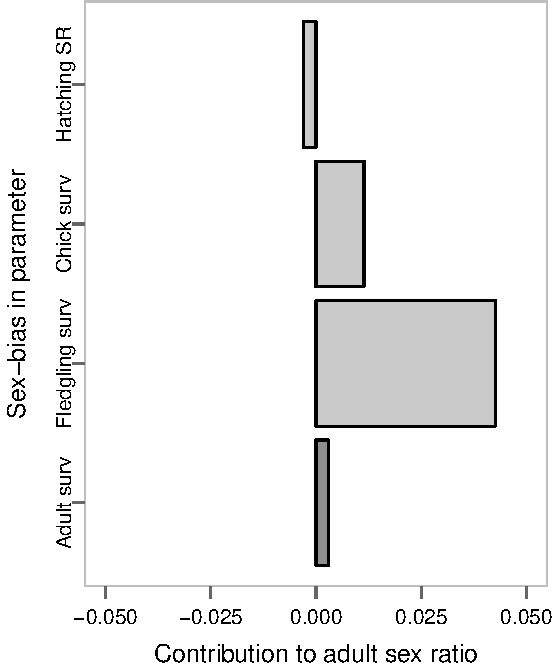
\includegraphics{Ceuta_ASR_Matrix_Modeling_files/figure-latex/unnamed-chunk-69-1} \end{center}

Determine how much larger the contribution of each vital rates is
compared to fledgling survival fledgling vs chick:

\begin{Shaded}
\begin{Highlighting}[]
\NormalTok{deterministic_LTRE$LTRE[}\DecValTok{2}\NormalTok{,}\DecValTok{5}\NormalTok{]/deterministic_LTRE$LTRE[}\DecValTok{1}\NormalTok{,}\DecValTok{5}\NormalTok{]}
\CommentTok{#> [1] 3.743087}
\end{Highlighting}
\end{Shaded}

fledgling vs adult:

\begin{Shaded}
\begin{Highlighting}[]
\NormalTok{deterministic_LTRE$LTRE[}\DecValTok{2}\NormalTok{,}\DecValTok{5}\NormalTok{]/deterministic_LTRE$LTRE[}\DecValTok{3}\NormalTok{,}\DecValTok{5}\NormalTok{]}
\CommentTok{#> [1] 14.25118}
\end{Highlighting}
\end{Shaded}

chick vs adult:

\begin{Shaded}
\begin{Highlighting}[]
\NormalTok{deterministic_LTRE$LTRE[}\DecValTok{1}\NormalTok{,}\DecValTok{5}\NormalTok{]/deterministic_LTRE$LTRE[}\DecValTok{3}\NormalTok{,}\DecValTok{5}\NormalTok{]}
\CommentTok{#> [1] 3.807333}
\end{Highlighting}
\end{Shaded}

\begin{center}\rule{0.5\linewidth}{\linethickness}\end{center}

\subsection{Quantifying mating system}\label{quantifying-mating-system}

To put our estimate of ASR in the context of breeding behavior, we
quantified sex-specific mating strategies and the reproductive success
of snowy plovers at our study site. Females of this species desert
broods to seek serial mates (Page et al. 2009). Thus, we expected that a
larger number of females would exhibit within-season polygamy than
males.

\textbf{Step one: wrangle the data} remove any cases in which one mate
was not identified (i.e., ``NA'')

\begin{Shaded}
\begin{Highlighting}[]
\NormalTok{mating_df <-}\StringTok{ }
\StringTok{  }\NormalTok{breeding_data[}\KeywordTok{which}\NormalTok{(!}\KeywordTok{is.na}\NormalTok{(breeding_data$female) &}\StringTok{ }\NormalTok{!}\KeywordTok{is.na}\NormalTok{(breeding_data$male)),]}
\end{Highlighting}
\end{Shaded}

bind the two mates together to make a unique pair

\begin{Shaded}
\begin{Highlighting}[]
\NormalTok{mating_df$pair <-}\StringTok{ }\KeywordTok{as.factor}\NormalTok{(}\KeywordTok{paste}\NormalTok{(mating_df$female, mating_df$male, }\DataTypeTok{sep =} \StringTok{"-"}\NormalTok{))}
\end{Highlighting}
\end{Shaded}

determine how many mating attempts each individual had each year

\begin{Shaded}
\begin{Highlighting}[]
\NormalTok{females <-}\StringTok{ }\NormalTok{reshape2::}\KeywordTok{dcast}\NormalTok{(mating_df, female  ~}\StringTok{ }\NormalTok{year)}
\NormalTok{males <-}\StringTok{ }\NormalTok{reshape2::}\KeywordTok{dcast}\NormalTok{(mating_df, male  ~}\StringTok{ }\NormalTok{year)}
\end{Highlighting}
\end{Shaded}

determine how many different mates each individual had over their
lifetime in the popualtion

\begin{Shaded}
\begin{Highlighting}[]
\NormalTok{number_males_p_female <-}\StringTok{ }
\StringTok{  }\NormalTok{stats::}\KeywordTok{aggregate}\NormalTok{(male ~}\StringTok{ }\NormalTok{female, mating_df, function(x) }\KeywordTok{length}\NormalTok{(}\KeywordTok{unique}\NormalTok{(x)))}
\NormalTok{number_females_p_male <-}\StringTok{ }
\StringTok{  }\NormalTok{stats::}\KeywordTok{aggregate}\NormalTok{(female ~}\StringTok{ }\NormalTok{male, mating_df, function(x) }\KeywordTok{length}\NormalTok{(}\KeywordTok{unique}\NormalTok{(x)))}
\end{Highlighting}
\end{Shaded}

join these two dataframes together and define as numeric

\begin{Shaded}
\begin{Highlighting}[]
\NormalTok{females <-}\StringTok{ }\NormalTok{dplyr::}\KeywordTok{inner_join}\NormalTok{(females, number_males_p_female)}
\NormalTok{females[,}\KeywordTok{c}\NormalTok{(}\DecValTok{2}\NormalTok{:}\DecValTok{8}\NormalTok{)] <-}\StringTok{ }
\StringTok{  }\KeywordTok{lapply}\NormalTok{(females[,}\KeywordTok{c}\NormalTok{(}\DecValTok{2}\NormalTok{:}\DecValTok{8}\NormalTok{)], as.numeric)}
\NormalTok{males <-}\StringTok{ }\NormalTok{dplyr::}\KeywordTok{inner_join}\NormalTok{(males, number_females_p_male)}
\NormalTok{males[,}\KeywordTok{c}\NormalTok{(}\DecValTok{2}\NormalTok{:}\DecValTok{8}\NormalTok{)] <-}\StringTok{ }
\StringTok{  }\KeywordTok{lapply}\NormalTok{(males[,}\KeywordTok{c}\NormalTok{(}\DecValTok{2}\NormalTok{:}\DecValTok{8}\NormalTok{)], as.numeric)}
\end{Highlighting}
\end{Shaded}

calculate the total number of mating attempts over each individual's
lifetime

\begin{Shaded}
\begin{Highlighting}[]
\NormalTok{females$attempts <-}\StringTok{ }\KeywordTok{rowSums}\NormalTok{(females[, }\KeywordTok{c}\NormalTok{(}\DecValTok{2}\NormalTok{:}\DecValTok{8}\NormalTok{)])}
\NormalTok{males$attempts <-}\StringTok{ }\KeywordTok{rowSums}\NormalTok{(males[, }\KeywordTok{c}\NormalTok{(}\DecValTok{2}\NormalTok{:}\DecValTok{8}\NormalTok{)])}
\end{Highlighting}
\end{Shaded}

calculate the number of years breeding

\begin{Shaded}
\begin{Highlighting}[]
\NormalTok{females$years <-}\StringTok{ }\KeywordTok{rowSums}\NormalTok{(females[, }\KeywordTok{c}\NormalTok{(}\DecValTok{2}\NormalTok{:}\DecValTok{8}\NormalTok{)] >}\StringTok{ }\DecValTok{0}\NormalTok{)}
\NormalTok{males$years <-}\StringTok{ }\KeywordTok{rowSums}\NormalTok{(males[, }\KeywordTok{c}\NormalTok{(}\DecValTok{2}\NormalTok{:}\DecValTok{8}\NormalTok{)] >}\StringTok{ }\DecValTok{0}\NormalTok{)}
\end{Highlighting}
\end{Shaded}

filter out all individuals that only had one mating attempt

\begin{Shaded}
\begin{Highlighting}[]
\NormalTok{females_no_1 <-}\StringTok{ }\NormalTok{dplyr::}\KeywordTok{filter}\NormalTok{(females, male  !=}\StringTok{ }\DecValTok{1} \NormalTok{|}\StringTok{ }\NormalTok{years !=}\StringTok{ }\DecValTok{1} \NormalTok{|}\StringTok{ }\NormalTok{attempts !=}\StringTok{ }\DecValTok{1}\NormalTok{)}
\NormalTok{males_no_1 <-}\StringTok{ }\NormalTok{dplyr::}\KeywordTok{filter}\NormalTok{(males, female  !=}\StringTok{ }\DecValTok{1} \NormalTok{|}\StringTok{ }\NormalTok{years !=}\StringTok{ }\DecValTok{1} \NormalTok{|}\StringTok{ }\NormalTok{attempts !=}\StringTok{ }\DecValTok{1}\NormalTok{)}
\end{Highlighting}
\end{Shaded}

tidy up dataframes then bind them together

\begin{Shaded}
\begin{Highlighting}[]
\NormalTok{females_no_1$sex <-}\StringTok{ "Female"}
\NormalTok{females_no_1$sex <-}\StringTok{ }\KeywordTok{as.factor}\NormalTok{(females_no_1$sex)}
\KeywordTok{colnames}\NormalTok{(females_no_1)[}\KeywordTok{c}\NormalTok{(}\DecValTok{1}\NormalTok{,}\DecValTok{9}\NormalTok{)] <-}\StringTok{ }\KeywordTok{c}\NormalTok{(}\StringTok{"focal"}\NormalTok{, }\StringTok{"mate"}\NormalTok{)}
\NormalTok{males_no_1$sex <-}\StringTok{ "Male"}
\NormalTok{males_no_1$sex <-}\StringTok{ }\KeywordTok{as.factor}\NormalTok{(males_no_1$sex)}
\KeywordTok{colnames}\NormalTok{(males_no_1)[}\KeywordTok{c}\NormalTok{(}\DecValTok{1}\NormalTok{,}\DecValTok{9}\NormalTok{)] <-}\StringTok{ }\KeywordTok{c}\NormalTok{(}\StringTok{"focal"}\NormalTok{, }\StringTok{"mate"}\NormalTok{)}
\NormalTok{mating <-}\StringTok{ }\KeywordTok{rbind}\NormalTok{(females_no_1, males_no_1)}
\end{Highlighting}
\end{Shaded}

determine if an individual was either: a) monogamous between years
(i.e.~only 1 mate in lifetime, with the number of attempts equaling the
number years mating) b) monogamous within years (i.e.~only 1 mate in
lifetime, with the number of attempts greater the number years mating)
c) polygamous between years (i.e.~more than one mate in lifetime, with
the number of attempts equaling the number years mating) d) polygamous
within years (i.e.~more than one mate in lifetime, with the number of
attempts greater the number years mating)

\begin{Shaded}
\begin{Highlighting}[]
\NormalTok{mating$status <-}\StringTok{ }\KeywordTok{ifelse}\NormalTok{(mating$mate ==}\StringTok{ }\DecValTok{1} \NormalTok{&}\StringTok{ }\NormalTok{mating$years ==}\StringTok{ }\NormalTok{mating$attempts, }
                        \StringTok{"Monogamous between years"}\NormalTok{,}
                    \KeywordTok{ifelse}\NormalTok{(mating$mate ==}\StringTok{ }\DecValTok{1} \NormalTok{&}\StringTok{ }\NormalTok{mating$years <}\StringTok{ }\NormalTok{mating$attempts, }
                               \StringTok{"Monogamous within years"}\NormalTok{,}
                            \KeywordTok{ifelse}\NormalTok{(mating$mate >}\StringTok{ }\DecValTok{1} \NormalTok{&}\StringTok{ }\NormalTok{mating$years ==}\StringTok{ }\NormalTok{mating$attempts, }
                                      \StringTok{"Polygamous between years"}\NormalTok{,}
                                  \KeywordTok{ifelse}\NormalTok{(mating$mate >}\StringTok{ }\DecValTok{1} \NormalTok{&}\StringTok{ }\NormalTok{mating$years <}\StringTok{ }\NormalTok{mating$attempts, }
                                             \StringTok{"Polygamous within years"}\NormalTok{, }\StringTok{"XXX"}\NormalTok{))))}
\end{Highlighting}
\end{Shaded}

calculate the number of mates per year

\begin{Shaded}
\begin{Highlighting}[]
\NormalTok{mating$no_mates_per_year <-}\StringTok{ }\NormalTok{mating$mate/mating$years}
\end{Highlighting}
\end{Shaded}

run chi-squared test of the sex-differences in polygamy rates

\begin{Shaded}
\begin{Highlighting}[]
\KeywordTok{chisq.test}\NormalTok{(}\KeywordTok{table}\NormalTok{(mating$sex, mating$status)[,}\KeywordTok{c}\NormalTok{(}\DecValTok{3}\NormalTok{,}\DecValTok{4}\NormalTok{)])}
\CommentTok{#> }
\CommentTok{#>  Pearson's Chi-squared test with Yates' continuity correction}
\CommentTok{#> }
\CommentTok{#> data:  table(mating$sex, mating$status)[, c(3, 4)]}
\CommentTok{#> X-squared = 15.05, df = 1, p-value = 0.0001047}
\end{Highlighting}
\end{Shaded}

run chi-squared test of the sex-differences in monogamy rates

\begin{Shaded}
\begin{Highlighting}[]
\KeywordTok{chisq.test}\NormalTok{(}\KeywordTok{table}\NormalTok{(mating$sex, mating$status)[,}\KeywordTok{c}\NormalTok{(}\DecValTok{1}\NormalTok{,}\DecValTok{2}\NormalTok{)])}
\CommentTok{#> }
\CommentTok{#>  Pearson's Chi-squared test with Yates' continuity correction}
\CommentTok{#> }
\CommentTok{#> data:  table(mating$sex, mating$status)[, c(1, 2)]}
\CommentTok{#> X-squared = 2.0102, df = 1, p-value = 0.1562}
\end{Highlighting}
\end{Shaded}

run chi-squared test of the sex-differences in mating behaviour rates

\begin{Shaded}
\begin{Highlighting}[]
\KeywordTok{chisq.test}\NormalTok{(}\KeywordTok{table}\NormalTok{(mating$sex, mating$status))}
\CommentTok{#> }
\CommentTok{#>  Pearson's Chi-squared test}
\CommentTok{#> }
\CommentTok{#> data:  table(mating$sex, mating$status)}
\CommentTok{#> X-squared = 19.979, df = 3, p-value = 0.0001714}
\end{Highlighting}
\end{Shaded}

set the factor levels for plotting

\begin{Shaded}
\begin{Highlighting}[]
\NormalTok{mating$status <-}\StringTok{ }\KeywordTok{factor}\NormalTok{(mating$status, }
                        \DataTypeTok{levels =} \KeywordTok{c}\NormalTok{(}\StringTok{"Monogamous within years"}\NormalTok{,}
                                   \StringTok{"Monogamous between years"}\NormalTok{,}
                                   \StringTok{"Polygamous between years"}\NormalTok{,}
                                   \StringTok{"Polygamous within years"}\NormalTok{))}
\end{Highlighting}
\end{Shaded}

determine the number of males and females used in the analysis

\begin{Shaded}
\begin{Highlighting}[]
\NormalTok{sample_sizes_sex <-}\StringTok{ }
\StringTok{  }\NormalTok{stats::}\KeywordTok{aggregate}\NormalTok{(focal ~}\StringTok{ }\NormalTok{sex, }\DataTypeTok{data =} \NormalTok{mating, }\DataTypeTok{FUN =} \NormalTok{function(x)\{}\KeywordTok{NROW}\NormalTok{(x)\})}
\end{Highlighting}
\end{Shaded}

define the color palatte to use in the plot

\begin{Shaded}
\begin{Highlighting}[]
\NormalTok{custom_pal <-}\StringTok{ }\KeywordTok{c}\NormalTok{(}\StringTok{"#7b3294"}\NormalTok{, }\StringTok{"#9E6BB1"}\NormalTok{, }\StringTok{"#91bfdb"}\NormalTok{, }\StringTok{"#4575b4"}\NormalTok{)}
\end{Highlighting}
\end{Shaded}

plot the sex-differences in mating behaviour

\begin{Shaded}
\begin{Highlighting}[]
\NormalTok{ggplot2::}\KeywordTok{ggplot}\NormalTok{() +}
\StringTok{          }\KeywordTok{geom_bar}\NormalTok{(}\DataTypeTok{position =} \StringTok{"fill"}\NormalTok{, }\DataTypeTok{alpha =} \FloatTok{0.75}\NormalTok{, }
                   \DataTypeTok{data =} \NormalTok{mating, }\KeywordTok{aes}\NormalTok{(}\DataTypeTok{x =} \NormalTok{sex, }\DataTypeTok{fill =} \NormalTok{status)) +}
\StringTok{          }\KeywordTok{geom_text}\NormalTok{(}\DataTypeTok{data =} \NormalTok{sample_sizes_sex, }\DataTypeTok{size =} \DecValTok{3}\NormalTok{, }
                    \KeywordTok{aes}\NormalTok{(}\DataTypeTok{y =} \KeywordTok{c}\NormalTok{(}\FloatTok{1.05}\NormalTok{, }\FloatTok{1.05}\NormalTok{), }\DataTypeTok{x =} \KeywordTok{c}\NormalTok{(}\FloatTok{1.11}\NormalTok{, }\FloatTok{2.11}\NormalTok{), }\DataTypeTok{label =} \NormalTok{focal)) +}
\StringTok{          }\KeywordTok{annotate}\NormalTok{(}\StringTok{"text"}\NormalTok{, }\DataTypeTok{x =} \KeywordTok{c}\NormalTok{(}\FloatTok{0.92}\NormalTok{, }\FloatTok{1.92}\NormalTok{), }\DataTypeTok{y =} \KeywordTok{c}\NormalTok{(}\FloatTok{1.05}\NormalTok{, }\FloatTok{1.05}\NormalTok{), }
                   \DataTypeTok{label =} \StringTok{"n = "}\NormalTok{, }\DataTypeTok{size =} \DecValTok{3}\NormalTok{) +}
\StringTok{          }\KeywordTok{theme_bw}\NormalTok{() +}
\StringTok{          }\KeywordTok{theme}\NormalTok{(}\DataTypeTok{legend.text =} \KeywordTok{element_text}\NormalTok{(}\DataTypeTok{size =} \DecValTok{10}\NormalTok{),}
                \DataTypeTok{legend.title =} \KeywordTok{element_blank}\NormalTok{(),}
                \DataTypeTok{legend.position =} \StringTok{"bottom"}\NormalTok{,}
                \DataTypeTok{legend.key.height=}\KeywordTok{unit}\NormalTok{(}\FloatTok{0.8}\NormalTok{,}\StringTok{"line"}\NormalTok{),}
                \DataTypeTok{legend.key.width=}\KeywordTok{unit}\NormalTok{(}\FloatTok{0.8}\NormalTok{,}\StringTok{"line"}\NormalTok{),}
                \DataTypeTok{axis.title.x =} \KeywordTok{element_blank}\NormalTok{(),}
                \DataTypeTok{axis.text.x  =} \KeywordTok{element_text}\NormalTok{(}\DataTypeTok{size =} \DecValTok{10}\NormalTok{), }
                \DataTypeTok{axis.title.y =} \KeywordTok{element_text}\NormalTok{(}\DataTypeTok{size =} \DecValTok{12}\NormalTok{, }\DataTypeTok{margin =} \KeywordTok{margin}\NormalTok{(}\DecValTok{0}\NormalTok{, }\DecValTok{15}\NormalTok{, }\DecValTok{0}\NormalTok{, }\DecValTok{0}\NormalTok{)),}
                \DataTypeTok{axis.text.y =} \KeywordTok{element_text}\NormalTok{(}\DataTypeTok{size =} \DecValTok{10}\NormalTok{), }
                \DataTypeTok{panel.grid.major =} \KeywordTok{element_blank}\NormalTok{(),}
                \DataTypeTok{panel.grid.minor =} \KeywordTok{element_blank}\NormalTok{(),}
                \DataTypeTok{strip.text.x =} \KeywordTok{element_text}\NormalTok{(}\DataTypeTok{size=}\DecValTok{12}\NormalTok{),}
                \DataTypeTok{strip.background =} \KeywordTok{element_blank}\NormalTok{(),}
                \DataTypeTok{strip.text =} \KeywordTok{element_text}\NormalTok{(}\DataTypeTok{vjust =} \NormalTok{-}\DecValTok{10}\NormalTok{),}
                \DataTypeTok{axis.ticks.x =} \KeywordTok{element_blank}\NormalTok{(),}
                \DataTypeTok{axis.ticks.y =} \KeywordTok{element_line}\NormalTok{(}\DataTypeTok{size =} \FloatTok{0.5}\NormalTok{, }\DataTypeTok{colour =} \StringTok{"grey40"}\NormalTok{),}
                \DataTypeTok{axis.ticks.length =} \KeywordTok{unit}\NormalTok{(}\FloatTok{0.2}\NormalTok{, }\StringTok{"cm"}\NormalTok{),}
                \DataTypeTok{panel.border =} \KeywordTok{element_rect}\NormalTok{(}\DataTypeTok{linetype =} \StringTok{"solid"}\NormalTok{, }\DataTypeTok{colour =} \StringTok{"grey"}\NormalTok{),}
                \DataTypeTok{plot.margin =} \KeywordTok{unit}\NormalTok{(}\KeywordTok{c}\NormalTok{(}\FloatTok{0.2}\NormalTok{,}\FloatTok{0.2}\NormalTok{,-}\FloatTok{0.2}\NormalTok{,}\FloatTok{0.2}\NormalTok{), }\StringTok{"cm"}\NormalTok{)) +}
\StringTok{          }\KeywordTok{ylab}\NormalTok{(}\StringTok{"Proportion of individuals"}\NormalTok{) +}
\StringTok{          }\KeywordTok{scale_fill_manual}\NormalTok{(}\DataTypeTok{values =} \NormalTok{custom_pal) +}
\StringTok{          }\KeywordTok{scale_y_continuous}\NormalTok{(}\DataTypeTok{limits =} \KeywordTok{c}\NormalTok{(}\DecValTok{0}\NormalTok{, }\FloatTok{1.05}\NormalTok{)) +}
\StringTok{          }\KeywordTok{guides}\NormalTok{(}\DataTypeTok{fill =} \KeywordTok{guide_legend}\NormalTok{(}\DataTypeTok{ncol =} \DecValTok{1}\NormalTok{, }\DataTypeTok{byrow =} \OtherTok{TRUE}\NormalTok{))}
\end{Highlighting}
\end{Shaded}

\begin{center}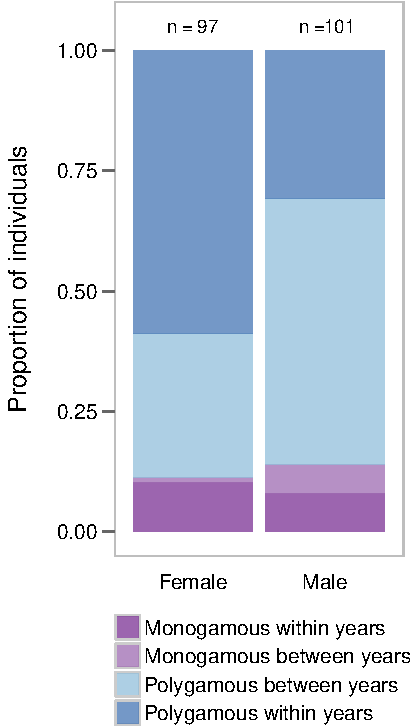
\includegraphics{Ceuta_ASR_Matrix_Modeling_files/figure-latex/unnamed-chunk-90-1} \end{center}

\begin{center}\rule{0.5\linewidth}{\linethickness}\end{center}

\subsection{R session information}\label{r-session-information}

\begin{Shaded}
\begin{Highlighting}[]
\KeywordTok{sessionInfo}\NormalTok{()}
\CommentTok{#> R version 3.3.0 (2016-05-03)}
\CommentTok{#> Platform: x86_64-apple-darwin13.4.0 (64-bit)}
\CommentTok{#> Running under: OS X 10.11.6 (El Capitan)}
\CommentTok{#> }
\CommentTok{#> locale:}
\CommentTok{#> [1] en_US.UTF-8/en_US.UTF-8/en_US.UTF-8/C/en_US.UTF-8/en_US.UTF-8}
\CommentTok{#> }
\CommentTok{#> attached base packages:}
\CommentTok{#> [1] grid      stats     graphics  grDevices utils     datasets  methods  }
\CommentTok{#> [8] base     }
\CommentTok{#> }
\CommentTok{#> other attached packages:}
\CommentTok{#>  [1] magrittr_1.5       lme4_1.1-12        Matrix_1.2-7.1    }
\CommentTok{#>  [4] Rmisc_1.5          plyr_1.8.4         lattice_0.20-34   }
\CommentTok{#>  [7] RColorBrewer_1.1-2 reshape2_1.4.1     gridExtra_2.2.1   }
\CommentTok{#> [10] dplyr_0.5.0        ggplot2_2.1.0      stringr_1.1.0     }
\CommentTok{#> [13] RMark_2.2.0       }
\CommentTok{#> }
\CommentTok{#> loaded via a namespace (and not attached):}
\CommentTok{#>  [1] Rcpp_0.12.7      formatR_1.4      nloptr_1.0.4     tools_3.3.0     }
\CommentTok{#>  [5] digest_0.6.10    evaluate_0.9     tibble_1.2       gtable_0.2.0    }
\CommentTok{#>  [9] nlme_3.1-128     DBI_0.5-1        yaml_2.1.13      parallel_3.3.0  }
\CommentTok{#> [13] mvtnorm_1.0-5    expm_0.999-0     coda_0.18-1      knitr_1.14      }
\CommentTok{#> [17] R6_2.1.3         survival_2.39-5  rmarkdown_1.0    minqa_1.2.4     }
\CommentTok{#> [21] scales_0.4.0     htmltools_0.3.5  matrixcalc_1.0-3 splines_3.3.0   }
\CommentTok{#> [25] MASS_7.3-45      assertthat_0.1   colorspace_1.2-6 labeling_0.3    }
\CommentTok{#> [29] stringi_1.1.1    lazyeval_0.2.0   munsell_0.4.3    msm_1.6.1}
\end{Highlighting}
\end{Shaded}

\end{document}
